\documentclass{article}

\usepackage{amsmath,geometry,graphicx,array,makecell,enumitem,bm,booktabs,multirow,pgfplots,amssymb,mathtools,nicematrix}
\usepackage[amsmath]{ntheorem}
\usepackage[hidelinks]{hyperref}
\usepackage[nameinlink,noabbrev]{cleveref}
\usepackage[makeroom]{cancel}
\usepackage{fancyhdr}
\pagestyle{fancy}
\fancyhead[L]{\itshape\nouppercase{\leftmark}}
\fancyhead[R]{B10 Electronic Structure}

\usetikzlibrary{decorations.pathreplacing}


\title{Electronic Structure}
\author{Yue Wu}

\geometry{a4paper,hmargin=1.1in,vmargin=1.2in}

\setlength{\parskip}{1em}
\tolerance=1000
\emergencystretch=1em
\hyphenpenalty=1000
\exhyphenpenalty=100
\righthyphenmin=3

\theoremstyle{plain}\theoremheaderfont{\normalfont\itshape}\theorembodyfont{\rmfamily}\theoremseparator{.}\newtheorem*{rem}{Remark}\newtheorem*{ex}{Example}\newtheorem*{proof}{Proof}\newtheorem*{altp}{Alternative proof}

\theoremstyle{plain}\theoremheaderfont{\normalfont\bfseries}\theorembodyfont{\rmfamily}\theoremseparator{.}\newtheorem{thm}{Theorem}[section]\newtheorem{lem}[thm]{Lemma}\newtheorem{prop}[thm]{Proposition}\newtheorem*{cor}{Corollary}\newtheorem{defn}[thm]{Definition}\newtheorem{clm}[thm]{Claim}\newtheorem{clminproof}{Claim}

\theoremstyle{break}\theoremheaderfont{\normalfont\itshape}\theorembodyfont{\rmfamily}\theoremseparator{.\medskip}\newtheorem*{proofskip}{Proof}\newtheorem*{exs}{Examples}\newtheorem*{rems}{Remarks}

\theoremstyle{break}\theoremheaderfont{\normalfont\bfseries}\theorembodyfont{\rmfamily}\theoremseparator{.\medskip}\newtheorem{lemskip}[thm]{Lemma}\newtheorem{defnskip}[thm]{Definition}\newtheorem{propskip}[thm]{Proposition}\newtheorem{thmskip}[thm]{Theorem}

\crefname{thm}{Theorem}{Theorems}\crefname{defn}{Definition}{Definitions}\crefname{lem}{Lemma}{Lemmas}\crefname{lemskip}{Lemma}{Lemmas}\crefname{cor}{Corollary}{Corollaries} \crefname{prop}{Proposition}{Propositions}\crefname{clm}{Claim}{Claims}

\setcounter{tocdepth}{2}
\numberwithin{equation}{section}
\counterwithin{figure}{section}

\NiceMatrixOptions{cell-space-limits = 2pt}

\newcommand{\qed}{\hfill\ensuremath{\Box}}
\newcommand{\unit}[1]{\ \mathrm{#1}}
\newcommand{\ii}{\mathrm{i}}
\newcommand{\e}{\mathrm{e}}
\newcommand{\tp}{^\mathrm{T}}
\newcommand{\dd}[2][]{\mathrm{d}^{#1} #2\,}
\renewcommand{\d}[2][]{\mathrm{d}^{#1} #2}
\newcommand{\dv}[3][]{\frac{\mathrm{d}^{#1} #2}{{\mathrm{d} #3}^{#1}}}
\newcommand{\pdv}[3][]{\frac{\partial^{#1} #2}{{\partial #3}^{#1}}}
\newcommand{\bra}[1]{\left\langle #1 \right|}
\newcommand{\ket}[1]{\left| #1 \right\rangle}
\newcommand{\braket}[2]{\left\langle #1 \middle| #2 \right\rangle}
\newcommand{\mel}[3]{\left\langle #1 \middle| #2 \middle| #3 \right\rangle}
\newcommand{\expval}[2]{\left\langle #2 \middle| #1 \middle| #2 \right\rangle}
\newcommand{\vb}[1]{\bm{\mathrm{#1}}}
\newcommand{\abs}[1]{\left| #1 \right|}
\newcommand{\norm}[1]{\left\| #1 \right\|}
\newcommand{\grad}{\vb{\nabla}}
\renewcommand{\div}{\vb{\nabla}\cdot}
\newcommand{\curl}{\vb{\nabla}\times}
\newcommand{\laplacian}{\nabla^2}
\newcommand{\bracket}[2]{\left( #1 \middle| #2 \right)}
\newcommand{\braccket}[2]{\left( #1 \middle\| #2 \right)}
\DeclareMathOperator*{\erf}{\operatorname{erf}}
\DeclareMathOperator{\antisymm}{\hat{\mathcal{A}}}
\newcommand{\ext}{_{\text{ext}}}
\newcommand{\ee}{_{\text{e-e}}}
\newcommand{\s}{_{\text{s}}}
\newcommand{\x}{_{\text{x}}}
\newcommand{\corr}{_{\text{c}}}
\newcommand{\xc}{_{\text{xc}}}
\newcommand{\rr}{\mathsf{r}}
\newcommand{\RR}{\mathsf{R}}
\newcommand{\inlineeqno}{\hfill\stepcounter{equation}\ (\theequation)}
\newcommand{\tikzxmark}{
\tikz[scale=0.23] {
    \draw[line width=0.7,line cap=round] (0,0) to [bend left=6] (1,1);
    \draw[line width=0.7,line cap=round] (0.2,0.95) to [bend right=3] (0.8,0.05);
}}
\newcommand{\tikzcmark}{
\tikz[scale=0.23] {
    \draw[line width=0.7,line cap=round] (0.25,0) to [bend left=10] (1,1);
    \draw[line width=0.8,line cap=round] (0,0.35) to [bend right=1] (0.23,0);
}}

\pgfplotsset{compat=1.18}

\begin{document}
    \setlength{\parindent}{0pt}
	\Huge\textsf{\textbf{Electronic Structure}}
		
	\Large\textsf{\textbf{University of Cambridge Part II Natural Sciences Tripos}}

	\noindent\makebox[\linewidth]{\rule{\textwidth}{2pt}}

	\large\textsf{\textbf{Yue Wu}}
	\begin{itemize}[topsep=0pt,leftmargin=15pt]
		\item[] \textit{Yusuf Hamied Department of Chemistry\\
		Lensfield Road,\\
		Cambridge, CB2 1EW}\\

		\textit{yw628@cam.ac.uk}
	\end{itemize}
    \thispagestyle{empty}
    \pagenumbering{roman}
    \setlength{\parindent}{15pt}

    \newpage
    \begin{center}
		\textbf{\Large{Acknowledgements}}
	\end{center}
	\large
	Nothing in these lecture notes is original. They are largely based on the notes by Dr. Alex Thom, who lectured this course in 2023 and 2024. They are nowhere near accurate representations of what was actually lectured, and in particular, all errors are almost surely mine.

    \normalsize
    \newpage
	\tableofcontents
	\newpage
    \pagenumbering{arabic}

    \part{\textit{Ab Initio} Quantum Chemistry}
    \section{The Hamiltonian and the Wavefunction}
    In these lectures, we shall use atomic units. These are defined as
    \begin{enumerate}[topsep=0pt,label=(\roman*)]
        \item unit of length is \textit{Bohr} \(a_0\), with dimension \(\mathrm{L}\);
        \item unit of charge is the magnitude of the charge on the electron \(e\), with dimension \(\mathrm{Q}\);
        \item unit of action is \textit{reduced Planck's constant} \(\hbar\), with dimension \(\mathrm{ML^2T^{-1}}\);
        \item unit of mass is the mass of the electron \(m_e\), with dimension \(\mathrm{M}\).
    \end{enumerate}
    These definitions imply that \(4\pi\epsilon_0=1\) because of the relation
    \begin{equation}
        a_0=\frac{4\pi\epsilon_0 \hbar^2}{m_e e^2}\,.
    \end{equation}
    In these units the unit of energy is \textit{Hartree} \(E_h\). The speed of light in atomic units is \(137.036\).

    In these units the molecular electronic Schr\"{o}dinger Hamiltonian, ignoring all relativistic terms, is
    \begin{equation}
        \hat{H}=-\frac{1}{2}\sum_{i=1}^{n}\laplacian_i-\sum_{i=1}^{n}\sum_{A=1}^{N}\frac{Z_A}{\norm{\vb{r}_i-\vb{R}_A}}+\sum_{i>j}^{n}\frac{1}{\norm{\vb{r}_i-\vb{r}_j}}+\sum_{A>B}^{N}\frac{Z_AZ_B}{\norm{\vb{R}_A-\vb{R}_B}}\,,
    \end{equation}
    where \(i,j\) label electrons at \(\vb{r}_i,\vb{r}_j\), and \(A,B\) label nuclei with charges \(Z_A,Z_B\) at \(\vb{R}_A,\vb{R}_B\). This part of the course is concerned with the determination of solutions (energies and wavefunctions) of the Schr\"{o}dinger equation
    \begin{equation}
        \hat{H}\Psi=E\Psi
    \end{equation}
    for fixed positions of the nuclei. This is formally known as the \textit{clamped-nucleus approximation}. Eigenvalue \(E\equiv E(\{\vb{R_i}\})\) as a function of nuclear positions \(\{\vb{R}_i\}\) is the \textit{potential energy surface}. This part of the course is on \textit{ab initio} quantum chemistry, meaning that we use no (semi-)empirical or experimental information.

    The fundamental expansion functions which we use to find approximate solutions of Schr\"{o}dinger's equation are \textit{Slater determinants}, which have the form
    \begin{equation}
        \Psi=\frac{1}{\sqrt{n!}}\begin{vmatrix}
            \phi_1(1) & \phi_1(2) & \cdots & \phi_1(n)\\
            \phi_2(1) & \phi_2(2) & \cdots & \phi_2(n)\\
            \vdots & \vdots & \ddots & \vdots \\
            \phi_n(1) & \phi_n(2) & \cdots & \phi_n(n)\\
        \end{vmatrix}\,,
    \end{equation}
    where \(i\) is the shorthand notation for spatial and spin coordinates \(\vb{x}_i=(\vb{r}_i,\omega_i)\).

    We can rewrite the Slater determinant into a form that is much easier to handle. But first, we need some knowledge of permutation groups.

    \begin{lem}
        Let \(X\) be a set.
        \begin{enumerate}[topsep=0pt,label=(\roman*)]
            \item The \textit{permutations} on \(X\), \(\hat{P}:X\to X\) form a group under function composition, which is known as the \textit{permutation group of \(X\)}.
            \item If \(X\) has \(n\) elements, then the permutation group on \(X\) is denoted \(S_n\). It has \(n!\) elements.
            \item A \textit{\(k\)-cycle} is a permutation
            \begin{equation}
                (a_1~a_2~\dots ~a_k)(i)=\begin{cases}
                    a_{j+1} & \text{if }i=a_j\text{ for }j<k\\
                    a_1 & \text{if }i=a_k\\
                    i & \text{if }i\ne a_j \text{ for any } j\,.
                \end{cases}
            \end{equation}
            A \textit{transposition} is a \(2\)-cycle.
            \item A permutation has a unique decomposition into disjoint cycles, and a \(k\)-cycle can be decomposed into \(k-1\) transpositions. Therefore, all permutations can be decomposed into transpositions.
            \item If a permutation \(\hat{P}_u\) can be decomposed into an even number of transpositions, then the permutation is said to have an even \textit{parity} \(\sigma_u=+1\). If it is decomposed into an odd number of transpositions, then it has an odd parity \(\sigma_u = -1\).
        \end{enumerate}
    \end{lem}
    We may rewrite the Slater determinant as
    \begin{equation}
        \Psi=\antisymm(\phi_1(1)\phi_2(2)\dots\phi_n(n))\,,
    \end{equation}
    where \(\antisymm\) is the \textit{antisymmetriser} defined as
    \begin{equation}
        \antisymm\coloneqq\frac{1}{\sqrt{n!}}\sum_{u\in S_n}^{n!}\sigma_u\hat{P}_u\,,
    \end{equation}
    in which \(\hat{P}_u\) is a \textit{permutation operator} that permutes the coordinates in the \textit{Hartree product} \(\Phi\coloneqq\phi_1(1)\phi_2(2)\dots\phi_n(n)\). For example, the permutation \(\hat{P}_{(i\ j)}\) permutes the coordinates of electron \(i\) and electron \(j\), so that
    \begin{align}
        \hat{P}_{(i\ j)}\Phi&=\hat{P}_{(i\ j)}\phi_1(1)\dots\phi_i(i)\dots\phi_j(j)\dots\phi_n(n)\notag\\
        &=\phi_1(1)\dots\phi_i(j)\dots\phi_j(i)\dots\phi_n(n)\,.
    \end{align}
    The antisymmetriser therefore sums over all possible permutations of the electron coordinates, multiplied by the parity of the permutations so that the result obeys the \textit{Pauli's exclusion principle}: a wavefunction changes sign on the interchange of the coordinates of two electrons. Note that these determinants are zero if
    \begin{enumerate}[topsep=0pt,label=(\roman*)]
        \item two spin-orbitals are the same (\(\phi_i=\phi_j\)), or
        \item the coordinates of two electrons are the same (\((\vb{r}_i,\omega_i)=(\vb{r}_j,\omega_j)\))
    \end{enumerate}
    as desired from Pauli's principle.

    \newpage
    \section{Basis Functions}
    Ideally it would be best to use hydrogenic type functions
    \begin{equation}
        R_{nl}(r)Y_{lm}(\theta,\phi)
    \end{equation}
    as expansion functions for molecular orbitals. Equivalently, these functions can be written as
    \begin{equation}
        r^nx^py^qz^s\exp(-Z_n r)\,,
    \end{equation}
    from which we can see that such a set includes \(\mathrm{s,p,d,f,\dots}\) hydrogenic atomic orbital wavefunctions. These functions are usually referred to as \textit{Slater functions}. However it is impossible to analytically evaluate the one and two electron integrals which arise in the evaluation of matrix elements if these functions are used. This means that to use them in computation, we need time-consuming and often inaccurate numerical integrations.
    \subsection{Gaussian Type Orbitals}
    Instead, computational quantum chemistry usually uses \textit{Gaussian basis functions}. They have the form
    \begin{equation}
        x^py^qz^s\exp(-ar^2)\,,
    \end{equation}
    where \(p,q,s\) are integers. The angular parts of these functions are the same as the Slater functions, but the radial part is different. The derivative of an \(\mathrm{s}\) Gaussian is zero at the origin, unlike the Slater function. Also the Gaussian dies off with \(\sim\exp(-a r^2)\) dependence compared to the Slater function's \(\sim\exp(-ar)\) dependence at large \(r\). Thus Gaussian functions have a totally different behaviour from Slater functions at both small \(r\) and large \(r\).

    \begin{figure}
        \centering
        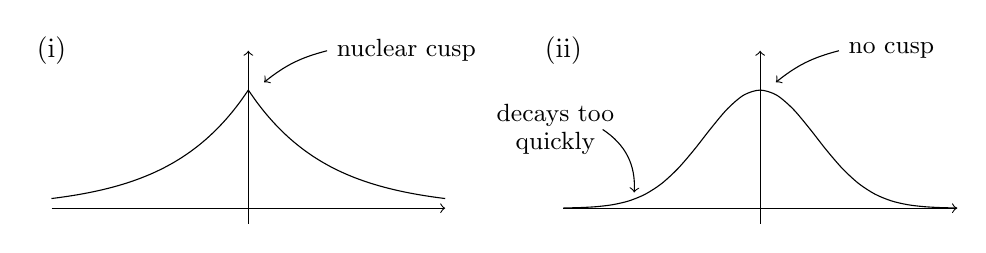
\begin{tikzpicture}
            \node at (-2.5,2) {(i)};
            \draw[->] (-2.5,0)--(2.5,0);
            \draw[->] (0,-0.2)--(0,2);
            \draw[domain=0:2.5, smooth, variable=\x] plot ({\x}, {1.5*2.72^(-\x)});
            \draw[domain=-2.5:0, smooth, variable=\x] plot ({\x}, {1.5*2.72^(\x)});
            \draw[->] (1,2) node[right]{\small nuclear cusp} to [bend right=12] (0.2,1.6);

            \node at (4,2) {(ii)};
            \draw[->] (4,0)--(9,0);
            \draw[->] (6.5,-0.2)--(6.5,2);
            \draw[domain=4:9, smooth, variable=\x] plot ({\x}, {1.5*2.72^(-(\x-6.5)^2)});
            \draw[->] (7.5,2) node[right]{\small no cusp} to [bend right=12] (6.7,1.6);
            \draw [->] (4.5,1) to [bend left=30] (4.9,0.2);
            \node[align=center] at (3.9,1) {\small decays too \\[-2pt] \small quickly};
        \end{tikzpicture}
        \caption{A comparison of (i) Slater type orbital and (ii) Gaussian function.}
        \label{Fig:coordsysaccobs}
    \end{figure}

    However the key advantage of Gaussians is that all the required integrals are very easy to evaluate. This follows from the fact that the product of two Gaussians is another Gaussian. This is known as the Gaussian product theorem.
    \begin{thm}[Gaussian product theorem]
        Let \(E\) be a Euclidean space with Euclidean norm \(\norm{\ \cdot \ }\), \(\vb{r},\vb{r}_A,\vb{r}_B\in E\) and \(\alpha,\beta\in\mathbb{R}\), \(\alpha,\beta>0\). Then 
        \begin{equation}
            \e^{-\alpha\norm{\vb{r}-\vb{r}_A}^2}\e^{-\beta\norm{\vb{r}-\vb{r}_B}^2}=c\e^{-\gamma\norm{\vb{r}-\vb{r}_P}^2}
        \end{equation}
        for some \(\gamma\in\mathbb{R}\), \(\vb{r}_P\in E\) and normalising factor \(c\in\mathbb{R}\).
    \end{thm}
    \begin{proof}
        \begin{figure}[ht!]
            \centering
            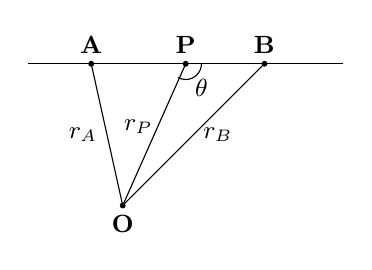
\begin{tikzpicture}
                \draw (0,0)--(4,0);
                \draw[fill=black] (0.8,0) circle (0.03) node[above]{\small \(\vb{A}\)};
                \draw[fill=black] (3,0) circle (0.03) node[above]{\small \(\vb{B}\)};
                \draw[fill=black] (2,0) circle (0.03) node[above]{\small \(\vb{P}\)};
                \draw[fill=black] (1.2,-1.8) circle (0.03) node[below]{\small \(\vb{O}\)};
                \draw (1.2,-1.8)--node[left]{\small \(r_A\)}(0.8,0);
                \draw (1.2,-1.8)--(2,0);
                \node at (1.4,-0.8) {\small \(r_P\)};
                \draw (1.2,-1.8)--node[right]{\small \(r_B\)}(3,0);
                \draw (2.2,0)arc(0:-120:0.2);
                \node at (2.2,-0.3) {\small \(\theta\)};
            \end{tikzpicture}
        \end{figure}
        Let \(\vb{P}\) be a point along \(\vb{AB}\). The cosine formula gives
        \begin{align}
            r_A^2 &= r_P^2+\norm{\vb{PA}}^2+2\norm{\vb{PA}}r_P\cos\theta\,,\\
            r_B^2 &= r_P^2+\norm{\vb{PB}}^2-2\norm{\vb{PB}}r_P\cos\theta\,.
        \end{align}
        If we choose the position \(\vb{P}\) such that \(\norm{\vb{PA}}/\norm{\vb{PB}}=\beta/\alpha\), that is
        \begin{equation}
            \vb{r}_P=\frac{\alpha\vb{r}_A+\beta\vb{r}_B}{\alpha+\beta}\,,
        \end{equation}
        then
        \begin{equation}
            \alpha r_A^2+\beta r_B^2=(\alpha+\beta)r_P^2+\alpha\norm{\vb{PA}}^2+\beta\norm{\vb{PB}}^2\,.
        \end{equation}
        Completing the algebra then gives the result
        \begin{equation}
            \e^{-\alpha r_A^2}\e^{-\beta r_B^2}=\e^{-\frac{\alpha\beta}{\alpha+\beta}\norm{\vb{AB}}^2}\e^{-(\alpha+\beta)r_P^2}
        \end{equation}
        as required.\qed
    \end{proof}
    The integrals of Gaussian functions are easily evaluated analytically.
    \begin{lem}[Gaussian integration lemma]
		For any constant \(a,b\in\mathbb{R}\) with \(a> 0\),
		\begin{equation}
            \int_{-\infty}^{\infty}\dd{u}\e^{-a(u+b)^2}=\sqrt{\frac{\pi}{a}}\,.
        \end{equation}
	\end{lem}
    It is then possible to evaluate the integrals that are needed for electronic structure calculation analytically. For example, the overlap integrals of two \(\mathrm{s}\) Gaussians are
    \begin{align}
        \braket{\eta_{A\alpha}}{\eta_{B\beta}}&\coloneqq\int\dd[3]{\vb{r}}\e^{-\alpha r_A^2}\e^{-\beta r_B^2}\notag\\
        &=\left(\frac{\pi}{\alpha+\beta}\right)^{\frac{3}{2}}\e^{-\frac{\alpha\beta}{\alpha+\beta}\norm{\vb{AB}}^2}\,.
    \end{align}
    The four-centre two-electron integral can also be evaluated:
    \begin{align}
        &\braket{\eta_{A\alpha}\eta_{C\gamma}}{\eta_{B\beta}\eta_{D\delta}}\equiv \bracket{\eta_{A\alpha}\eta_{B\beta}}{\eta_{C\gamma}\eta_{D\delta}}\notag\\
        \coloneqq&\iint\dd[3]{\vb{r}_1}\dd[3]{\vb{r}_2}\frac{\e^{-\alpha r_{1A}^2}\e^{-\beta r_{1B}^2}\e^{-\gamma r_{2C}^2}\e^{-\delta r_{2D}^2}}{r_{12}}\notag\\
        =&\braket{\eta_{A\alpha}}{\eta_{B\beta}}\braket{\eta_{C\gamma}}{\eta_{D\delta}}\erf\left(\left[\frac{(\alpha+\beta)(\gamma+\delta)}{\alpha+\beta+\gamma+\delta}\right]^{\frac{1}{2}}\norm{\vb{PQ}}\right)\,,
    \end{align}
    where
    \begin{equation}
        \vb{r}_P=\frac{\alpha\vb{r}_A+\beta\vb{r}_B}{\alpha+\beta}\,,\;\vb{r}_Q=\frac{\gamma\vb{r}_C+\delta\vb{r}_D}{\gamma+\delta}
    \end{equation}
    and
    \begin{equation}
        \erf(x)\coloneqq\frac{2}{\sqrt{\pi}}\int_{0}^{x}\dd{t}\exp(-t^2)
    \end{equation}
    is the \textit{error function}. This is more often quoted in an equivalent form in the literature
    \begin{equation}
        \braket{\eta_{A\alpha}\eta_{C\gamma}}{\eta_{B\beta}\eta_{D\delta}}=\frac{2\pi^{5/2}}{pq\sqrt{p+q}}F_0(\rho\norm{\vb{PQ}}^2)\,,
    \end{equation}
    where \(p=\alpha+\beta\), \(q=\gamma+\delta\), \(\rho=pq/(p+q)\) and
    \begin{equation}
        F_n(x)=\int_{0}^{1}\dd{t}\exp(-xt^2)t^{2n}
    \end{equation}
    is the \(n^{\text{th}}\)-order Boys function. You don't need to know any of the formulae above. You only need to appreciate that they exist, and computers can use them to quickly get the results of the integrals.
    \subsection{Standard Basis Sets}
    To overcome the difficulty of the less desirable short and long range behaviour of Gaussians, it is common today to use fixed combinations of one to six Gaussians as basis functions, with the combinations chosen such that they look more like Slater functions.
    
    These combinations are established, and there are a variety of different notations, usually referred to by the primary author who devised and published them. Here we will give a few examples:
    \begin{itemize}[topsep=0pt,parsep=1em]
        \item STO-3G (Pople) means the use of a contracted combination of three Gaussians to represent each Slater function. \(\mathrm{H}\) requires 1 s basis function made from 3 Gaussian functions. \(\mathrm{Li-Ne}\) require 2 s basis functions and one set of three p basis functions, so there are in total 5 of them, each made up from 3 Gaussian functions.
        
        \begin{figure}[ht!]
            \centering
            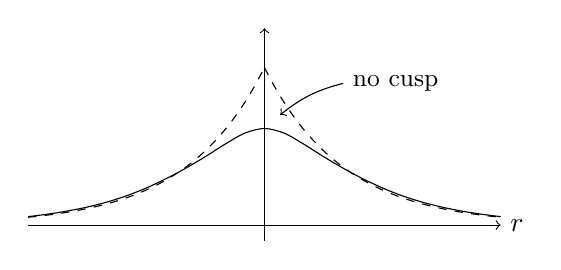
\begin{tikzpicture}
                \draw[->] (-3,0)--(3,0) node[right]{\(r\)};
                \draw[->] (0,-0.2)--(0,2.5);
                \draw[domain=0:3, smooth, variable=\x,dashed] plot ({\x}, {2*2.72^(-\x)});
                \draw[domain=-3:0, smooth, variable=\x,dashed] plot ({\x}, {2*2.72^(\x)});
                \draw[domain=-3:3, smooth, variable=\x] plot ({\x}, {0.1669*2.72^(-3.425*\x*\x) + 0.579*2.72^(-0.6239*\x*\x) + 0.481*2.72^(-0.1689*\x*\x)});
                \draw[->] (1,1.8) node[right]{\small no cusp} to [bend right=12] (0.2,1.4);
            \end{tikzpicture}
            \caption{STO-3G uses 3 Gaussian functions to mimic the Slater type hydrogen 1s orbital.}
        \end{figure}
        
        You can find the parameters of these basis functions on Basis Set Exchange.\footnote{\href{https://www.basissetexchange.org/}{\color{blue}https://www.basissetexchange.org/}} For example, if you search for the parameters of Li, you will get
        \begin{verbatim}
            #BASIS SET: (6s,3p) -> [2s,1p]
            Li    S
                0.1611957475E+02       0.1543289673E+00
                0.2936200663E+01       0.5353281423E+00
                0.7946504870E+00       0.4446345422E+00
            Li    SP
                0.6362897469E+00      -0.9996722919E-01       0.1559162750E+00
                0.1478600533E+00       0.3995128261E+00       0.6076837186E+00
                0.4808867840E-01       0.7001154689E+00       0.3919573931E+00
            END
        \end{verbatim}
        Let's have a close look at what everything means.

        The first section gives the parameters of the 3 Gaussians composing Li 1s orbitals:
        \begin{equation}
            \eta_{\mathrm{Li, 1s}}=\sum_{i=1}^{3} c_i \e^{-a_i r^2}\,,
        \end{equation}
        where
        \begin{table}[ht!]
            \centering
            \begin{tabular}{ccc}
                \toprule
                \(i\) & \(a_i\,/\, a_0^{-2}\) & \(c_i\) \\ \midrule
                1 & 16.11957475 & 0.1543289673 \\
                2 & 2.936200663 & 0.5353281423 \\
                3 & 0.7946504870 & 0.4446345422 \\ \bottomrule
            \end{tabular}
        \end{table}

        The second section gives the 3 Gaussians shared by the 2s and 2p orbitals:
        \begin{equation}
            \eta_{\mathrm{Li, 2s}}=\sum_{i=1}^{3} c_i^{(\mathrm{s})} \e^{-a_i r^2}\,,
        \end{equation}
        and
        \begin{equation}
            \eta_{\mathrm{Li}, 2\mathrm{p}_q}=\sum_{i=1}^{3} q c_i^{(\mathrm{p})} \e^{-a_i r^2}\,,
        \end{equation}
        where \(q\in\{x,y,z\}\) are Cartesian functions and parameters are
        \begin{table}[ht!]
            \centering
            \begin{tabular}{cccc}
                \toprule
                \(i\) & \(a_i\,/\, a_0^{-2}\) & \(c_i^{\mathrm{s}}\) & \(c_i^{\mathrm{p}}\) \\ \midrule
                1 & 0.6362897469 & \(-0.09996722919\) & 0.1559162750 \\
                2 & 0.1478600533 & 0.3995128261 & 0.6076837186 \\
                3 & 0.04808867840 & 0.7001154689 & 0.3919573931 \\ \bottomrule
            \end{tabular}
        \end{table}

        Note that the Gaussian functions are the same for 2s and 2p orbitals.

        Such a basis set is described as a \textit{minimal basis set} as it uses one basis function per atomic orbital.
        \item 6-31G* (Pople) is a \textit{split valence basis set}, in which a valence atomic orbital is split into two basis functions to allow more flexibility. It has 6 Gaussians in the core orbital and 3 and 1 Gaussians in the two valence orbitals. Moreover, due to the chemical environments, the electron density in an atom may be distorted. This requires us to bring in some orbitals with higher angular momentum for polarisation. To distort an s orbital, we need to introduce a p orbital, and to distort a p orbital, we need to use d orbitals \textit{etc.} The star means polarisation functions on all atoms except hydrogen, and ** would also add polarisation to hydrogen.
        \begin{figure}[ht!]
            \centering
            \begin{tikzpicture}
                \node at (-0.4,1) {(i)};
                \draw (0,0) circle (0.35) node{\scriptsize H};
                \draw[dashed] (0.4,0)--(1.8,0)node[right]{\scriptsize F};
                \node at (3.6,1) {(ii)};
                \node at (4,0) {\scriptsize H};
                \draw[dashed] (4.45,0)--(5.8,0)node[right]{\scriptsize F};
                \draw plot [smooth cycle, tension=1] coordinates { (3.8,0) (4.15,0.35) (4.43,0) (4.15,-0.35) };
            \end{tikzpicture}
            \caption{A hydrogen atom (i) without polarisation and (ii) with polarisation. The polarisation can be achieved by using an extra set of p orbitals.}
        \end{figure}

        A hydrogen atom has a 1s valence orbital, so 6-31G* would split it into two basis functions, composed of 3 and 1 Gaussians respectively. For Li-Ne, the 1s core orbital is made up from 6 Gaussians, while the 2s and 2p valence orbitals are each split into 2 basis functions composed of 3 and 1 Gaussians respectively. Moreover, polarisation introduces a set of d orbitals. Hence they are described by 15 basis functions (3s2p1d, and there are 6 d orbitals in 6-31G* --- see later).
        \item  cc-pVTZ (Dunning) is a large basis set for Hartree--Fock and is primarily designed for correlated methods. It stands for correlation consistent polarised valence triple zeta (e.g. H 3s2p1d (14 functions) Li-Ne 4s3p2d1f (30 functions)). Larger basis sets are available e.g. cc-pVQZ or cc-pV5Z.
        \item Augmented functions for diffuse basis sets for the description of anionic systems are e.g. aug-cc-pVTZ (Dunning) or 6-311++G(3df,3pd) (Pople).
        \item cc-pCVTZ (Dunning) includes functions for correlating core electrons.
    \end{itemize}
    \subsubsection{Cartesian vs Spherical}
    For d functions and beyond, the Cartesian function \(\{x_ix_j\}\) spans a larger space than the spherical harmonics \(\{2z^2-x^2-y^2,x^2-y^2,xy,xz,yz\}\). Care should be taken as to which definition is used within a basis set. The Pople 6-31G family use Cartesian d-functions, but spherical functions for f orbitals and beyond. Dunning style cc-pVXZ basis sets use purely spherical harmonics.
    \subsection{Slater Type Orbitals (Non-examinable)}
    A normalised Slater basis function is defined by
    \begin{equation}
        S(\zeta,n,\ell,m;r,\theta,\phi)=\frac{(2\zeta)^{n+\frac{1}{2}}}{[(2n)!]^{\frac{1}{2}}}r^{n-1}\e^{-\zeta r}Z_{\ell m}(\theta,\phi)\,.
    \end{equation}
    Thus they are defined through their exponent \(\zeta\), principal quantum number \(n\), angular momentum quantum number \(\ell\) and the magnetic quantum number \(m\). We have \(n>\ell\) and \(m=-\ell,-\ell+1,\dots,\ell\). \(Z_{\ell m}(\theta,\phi)\) are the real spherical harmonics given by
    \begin{equation}
        Z_{\ell,m}(\theta,\phi)=\left(\frac{(2\ell+1)(\ell-\abs{m})!}{2\pi(\ell+\abs{m})!}\right)^{\frac{1}{2}}\begin{cases}
            \cos(\abs{m}\phi)P_{\ell}^{\abs{m}}(\cos\theta) & \ell\ge m>0\\
            \frac{1}{\sqrt{2}}P_{\ell}^{0}(\cos\theta) & m=0\\
            \sin(\abs{m}\phi)P_{\ell}^{\abs{m}}(\cos\theta) & -\ell\le m<0\,,
        \end{cases}
    \end{equation}
    where \(P_\ell^m\) are the \textit{associated Legendre functions}.

    The formulae for the analytic potential of a STO are given by
    \begin{equation}
        V(\zeta,n,\ell,m;r,\theta,\phi)=\int_{0}^{\infty}\dd{r'}\int_{0}^{\pi}\dd{\theta'}\int_{0}^{2\pi}\dd{\phi'}\frac{S(\zeta,n,\ell,m;r',\theta',\phi')}{\norm{\vb{r}-\vb{r}'}}r'^2\sin\theta'\,.
    \end{equation}
    Using the well-known expansion of \(\norm{\vb{r}-\vb{r}'}\) in spherical harmonics, the following result is obtained
    \begin{equation}
        V(\zeta,n,\ell,m;r,\theta,\phi)=\frac{4\pi(2\zeta)^{n+\frac{1}{2}}}{[(2n)!]^{\frac{1}{2}}(2\ell+1)}Z_{\ell m}(\theta,\phi)I_{n\ell}(r)\,,
    \end{equation}
    with
    \begin{equation}
        I_{n\ell}(r)=r^{-\ell-1}\int_{0}^{r}\dd{r'}(r')^{n+\ell+1}\e^{-\zeta r'}+r^{\ell}\int_{r}^{\infty}\dd{r'}(r')^{n-\ell}\e^{-\zeta r'}\,.
    \end{equation}
    Both of these integrals may be evaluated recursively.

    The only other formula that is often used is the Laplacian of an STO
    \begin{equation}
        \laplacian S(\zeta,n,\ell,m;r,\theta,\phi)=[[n(n-1)-\ell(\ell+1)]r^{-2}-2n\zeta r^{-1}+\zeta^2]S(\zeta,n,\ell,m;r,\theta,\phi)\,.
    \end{equation}

    \newpage
    \section{Matrix Element of Determinants and Energy Expressions}
    We write the Slater determinant of a set of orthonormal spin-orbitals in the form
    \begin{align}
        \Psi&=\frac{1}{\sqrt{n!}}\begin{vmatrix}
            \phi_1(1) & \phi_1(2) & \cdots & \phi_1(n)\\
            \phi_2(1) & \phi_2(2) & \cdots & \phi_2(n)\\
            \vdots & \vdots & \ddots & \vdots \\
            \phi_n(1) & \phi_n(2) & \cdots & \phi_n(n)
        \end{vmatrix}\notag\\
        &=\antisymm(\phi_1\phi_2\dots\phi_n)\notag\\
        &=\antisymm\Phi\,.
    \end{align}

    We now work out some properties of \(\antisymm\) that may help us evaluate the matrix elements.
    \begin{lemskip}
        \begin{enumerate}[topsep=0pt,label=(\roman*)]
            \item \(\antisymm^2=\sqrt{n!}\antisymm\).
            \item \(\hat{P}_u\) is unitary, and so \(\antisymm\) is Hermitian, i.e. \(\braket{\antisymm\Phi}{\Psi}=\braket{\Phi}{\antisymm\Psi}\) for any \(\Phi,\Psi\).
            \item \(\expval{\hat{H}}{\antisymm\Phi}=\sqrt{n!}\mel{\Phi}{\hat{H}}{\antisymm\Phi}\).
        \end{enumerate}
    \end{lemskip}
    \begin{proofskip}
        \begin{enumerate}[topsep=0pt,label=(\roman*)]
            \item We have
            \begin{align}
                \antisymm^2&=\frac{1}{n!}\sum_{u}^{n!}\sigma_u\hat{P}_u\sum_{v}^{n!}\sigma_v\hat{P}_v\notag\\
                &=\frac{1}{n!}\sum_{u}^{n!}\sum_{v}^{n!}(\sigma_u\sigma_v)(\hat{P}_u\hat{P}_v)\,.
            \end{align}
            We need a simple result from group theory known as the \textit{rearrangement theorem}. It states that for any element \(g\) in a group \(G\), \(gG=\{gh\mid h\in G\}=G\). So, for each \(\hat{P}_u\)
            \begin{equation}
                \sum_{v\in S_n}\sigma_u\sigma_v\hat{P}_u\hat{P}_v=\sum_{w\in S_n}\sigma_w\hat{P}_w\,.
            \end{equation}
            This basically says that doing all possible permutations then do a specific permutation is equivalent to doing all possible permutations. Therefore,
            \begin{align}
                \antisymm^2&=\frac{1}{n!}\sum_{u,w}^{n!}\sigma_w\hat{P}_w\notag\\
                &=\frac{1}{n!}n!\sqrt{n!}\antisymm\notag\\
                &=\sqrt{n!}\antisymm\,.
            \end{align}
            Note that this is different from a projection operator, for which \(\hat{Q}^2=\hat{Q}\).
            \item \(\hat{P}_u\) is unitary because
            \begin{align}
                \braket{\hat{P}_u\Phi}{\Psi}&=\braket{\hat{P}_u^{-1}\hat{P}_u\Phi}{\hat{P}_u^{-1}\Psi}\notag\\
                &=\braket{\Phi}{\hat{P}_{u}^{-1}\Psi}
            \end{align}
            as acting the same permutation on both sides only introduces a relabelling of the integration variable. Note that \(\hat{P}_u\) and \(\hat{P}_{u}^{-1}\) have the same parity since parity \(\sigma:S_n\to C_2\) is a homomorphism and \(\sigma(\hat{P}_u^{-1})\sigma(\hat{P}_u)=\sigma(\hat{E})=1\). Therefore we have
            \begin{align}
                \braket{\sum_u\sigma_u\hat{P}_u\Phi}{\Psi}&=\braket{\Phi}{\sum_u\sigma_u\hat{P}_u^{-1}\Psi}\notag\\
                &=\braket{\Phi}{\sum_u\sigma_u\hat{P}_u\Psi}\,.
            \end{align}
            Hence
            \begin{equation}
                \braket{\antisymm\Phi}{\Psi}=\braket{\Phi}{\antisymm\Psi}\,.
            \end{equation}
            \item From (ii), we have
            \begin{equation}
                \expval{\hat{H}}{\antisymm\Phi}=\braket{\Phi}{\antisymm\hat{H}\antisymm\Phi}\,.
            \end{equation}
            \(\hat{H}\) is a symmetric operator that is invariant under the swapping of any pair of labels, so \(\hat{H}\) commutes with \(\antisymm\). Thus we have
            \begin{equation}
                \expval{\hat{H}}{\antisymm\Phi}=\mel{\Phi}{\hat{H}}{\antisymm^2\Phi}=\mel{\Phi}{\hat{H}}{\sum_u\sigma_u\hat{P}_u\Phi}
            \end{equation}
            as claimed. This is a significant simplification as we have reduced a sum of \((n!)^2\) terms to a sum of \(n!\) terms.\qed
        \end{enumerate}
    \end{proofskip}
    \begin{thm}\label{HF_Hamiltonian_expval}
        For a general Hamiltonian
        \begin{equation}
            \hat{H}=C+\sum_i \hat{h}(i)+\sum_{i>j}\frac{1}{r_{ij}}\,,
        \end{equation}
        the expected value of \(\hat{H}\) for the Slater determinant \(\Psi=\antisymm\Phi\) is given by
        \begin{equation}
            \expval{\hat{H}}{\Psi}=C+\sum_{i}h_{ii}+\sum_{i>j}[\bracket{ii}{jj}-\bracket{ij}{ij}]\,,
        \end{equation}
        where \(h_{ij}\) is the matrix element \(\mel{\phi_i}{\hat{h}}{\phi_j}\) and
        \begin{equation}
            \mel{\phi_i(1)\phi_j(2)}{\frac{1}{r_{12}}}{\phi_k(1)\phi_l(2)}\coloneqq\braket{ij}{kl}\equiv\bracket{ik}{jl}\,.
        \end{equation}
        The notation \(\braket{\ \cdot \ }{\ \cdot \ }\) is the \textit{physicists' notation} and \(\bracket{\ \cdot \ }{\ \cdot \ }\) is the \textit{chemists' notation}.
    \end{thm}
    \begin{proof}
        We consider each term of the operator in turn.
        \begin{enumerate}[topsep=0pt,label=(\roman*)]
            \item First the constant term \(C\):
            \begin{equation}
                \expval{C}{\Psi}=C\braket{\phi_1(1)\phi_2(2)\dots\phi_n(n)}{\sum_{u}\sigma_u\hat{P}_u\phi_1(1)\phi_2(2)\dots\phi_n(n)}\,.
            \end{equation}
            If \(\hat{P}_u=\hat{E}\), the identity operation, then the contribution is
            \begin{equation}
                C\braket{\phi_1}{\phi_1}_1\braket{\phi_2}{\phi_2}_2\dots\braket{\phi_n}{\phi_n}_n=C\,.
            \end{equation}
            If \(\hat{P}_u=\hat{P}_{12}\), we obtain the contribution
            \begin{equation}
                -C\cancelto{0}{\braket{\phi_1}{\phi_2}_1}\cancelto{0}{\braket{\phi_2}{\phi_1}_2}\dots\braket{\phi_n}{\phi_n}_n=0\,.
            \end{equation}
            Similarly, if \(\hat{P}_u\) is any non-identity permutation, it will permute some \(i\) to some \(j\ne i\), then the contribution is
            \begin{equation}
                \sigma_u C\dots\cancelto{0}{\braket{\phi_i}{\phi_j}_i}{\dots}=0\,.
            \end{equation}
            Therefore, only the identity permutation in the sum contributes and so
            \begin{equation}
                \expval{C}{\Psi}=C\,.
            \end{equation}
            Moreover, let \(C=1\) then \(\braket{\Psi}{\Psi}=1\) so we can check that the Slater determinant \(\Psi\) is normalised.

            \item Next, consider the one-electron Hamiltonian term \(\hat{h}(i)\):
            \begin{equation}
                \expval{\hat{h}(i)}{\Psi}=\mel{\phi_1(1)\phi_2(2)\dots\phi_n(n)}{\hat{h}(i)}{\sum_u\sigma_u\hat{P}_u\phi_1(1)\phi_2(2)\dots\phi_n(n)}\,.
            \end{equation}
            If \(\hat{P}_u=\hat{E}\), we obtain the contribution
            \begin{equation}
                \braket{\phi_1}{\phi_1}_1\braket{\phi_2}{\phi_2}_2\dots\expval{\hat{h}}{\phi_i}_i\dots\braket{\phi_n}{\phi_n}_n=\expval{\hat{h}}{\phi_i}\eqqcolon h_{ii}\,.
            \end{equation}
            If \(\hat{P}_u=\hat{P}_{ij}\), we obtain the contribution
            \begin{equation}
                -\braket{\phi_1}{\phi_1}_1\dots\mel{\phi_i}{\hat{h}}{\phi_j}_i\dots\cancelto{0}{\braket{\phi_j}{\phi_i}_i}\dots\braket{\phi_n}{\phi_n}_n=0\,,
            \end{equation}
            and the contribution from other terms vanish similarly. Thus summing over \(i\), we obtain
            \begin{equation}
                \expval{\sum_i\hat{h}(i)}{\Psi}=\sum_i h_{ii}\,.
            \end{equation}
            \item Finally, there is the \(e^- - e^-\) repulsion term \(\frac{1}{r_{ij}}\):
            \begin{equation}
                \expval{\frac{1}{r_{ij}}}{\Psi}=\mel{\phi_1(1)\phi_2(2)\dots\phi_n(n)}{\frac{1}{r_{ij}}}{\sum_u\sigma_u\hat{P}_u\phi_1(1)\phi_2(2)\dots\phi_n(n)}\,.
            \end{equation}
            If \(\hat{P}_u=\hat{E}\), we obtain the contribution
            \begin{equation}
                \braket{\phi_1}{\phi_1}_1\braket{\phi_2}{\phi_2}_2\dots\expval{\frac{1}{r_{ij}}}{\phi_i(i)\phi_j(j)}_{ij}\dots\braket{\phi_n}{\phi_n}_n=\bracket{ii}{jj}\,.
            \end{equation}
            If \(\hat{P}_u=\hat{P}_{ij}\), we obtain the contribution
            \begin{equation}
                -\braket{\phi_1}{\phi_1}_1\dots\mel{\phi_i(i)\phi_j(j)}{\frac{1}{r_{ij}}}{\phi_i(j)\phi_j(i)}_{ij}\dots\braket{\phi_n}{\phi_n}_n=-\bracket{ij}{ij}\,.
            \end{equation}
            Any other permutation will involve the overlap of different orbitals and hence give zero contribution. Thus summing over \(i>j\), we obtain
            \begin{equation}
                \expval{\frac{1}{r_{ij}}}{\Psi}=\sum_{i>j}[\bracket{ii}{jj}-\bracket{ij}{ij}]\,.
            \end{equation}
        \end{enumerate}

        Hence, the Slater determinant constructed from a Hartree product of normalised spin-orbitals \(\Psi=\antisymm\Phi\) is also normalised and
        \begin{equation}
            \expval{\hat{H}}{\Psi}=C+\sum_i h_{ii}+\sum_{i>j}[\bracket{ii}{jj}-\bracket{ij}{ij}]\,.
        \end{equation}
        \(\bracket{ii}{jj}\) is known as the \textit{Coulomb integral} and \(\bracket{ij}{ij}\) is the \textit{exchange integral}.\qed
    \end{proof}

    \begin{prop}\label[prop]{energy_invariance_unitary_rotation}
        The expectation value of a Slater determinant for an arbitrary operator \(\hat{Q}\) is invariant to a unitary rotation of its orbitals.
    \end{prop}
    \begin{proof}
        Let \(\Psi=\antisymm\phi_1\dots\phi_n\), where \(\{\phi_i\}_{i=1}^{n}\) are orthonormal, and let \(\vb{\psi}=\mathsf{U}\vb{\phi}\), where \(\mathsf{U}\) is unitary so that
        \begin{equation}
            \mathsf{U}^\dagger=\mathsf{U}^{-1}\,,\; \abs{\det\mathsf{U}}=1\,.
        \end{equation}
        In component form,
        \begin{equation}
            \psi_i=\sum_{j=1}^{n}U_{ij}\phi_j\,.
        \end{equation}
        Let the Slater determinant of the transformed orbital be
        \begin{align}
            \Psi'&=\antisymm\psi_1\dots\psi_n\notag\\
            &=\antisymm\sum_{j_1=1}^{n}U_{1j_1}\phi_{j_1}(1)\sum_{j_2=1}^{n}U_{2j_2}\phi_{j_2}(2)\dots\sum_{j_n=1}^{n}U_{nj_n}\phi_{j_n}(n)\notag\\
            &=\underbrace{\sum_{j_1=1}^{n}\sum_{j_2=1}^{n}\dots\sum_{j_n=1}^{n}}_{n^n\text{ terms}}U_{1j_1}U_{2j_2}\dots U_{nj_n}\antisymm\phi_{j_1}(1)\phi_{j_2}(2)\dots\phi_{j_n}(n)\,.
        \end{align}
        By the property of the antisymmetriser,
        \begin{equation}
            \antisymm\phi_{j_1}(1)\phi_{j_2}(2)\dots\phi_{j_n}(n)\ne 0
        \end{equation}
        if and only if \(\{1,2,\dots,n\}=\{j_1,j_2,\dots,j_n\}\). Thus, for a term in the sum to be non-zero, we must have
        \begin{equation}
            \phi_{j_1}(1)\phi_{j_2}(2)\dots\phi_{j_n}(n)=\hat{P}_{j_1\dots j_n}\phi_1(1)\phi_2(2)\dots\phi_n(n)\,.
        \end{equation}
        Hence,
        \begin{align}
            \Psi'&=\sum_{\hat{P}_{j_1\dots j_n}}^{n!}U_{1j_1}\dots U_{nj_n}\underbrace{\antisymm\hat{P}_{j_1\dots j_n}}_{\antisymm\hat{P}_{j_1\dots j_n}=\sigma_{j_1\dots j_n}\antisymm}\phi_1(1)\dots\phi_n(n)\notag\\
            &=\underbrace{\sum_{\hat{P}_{j_1\dots j_n}}^{n!}U_{1j_1}\dots U_{nj_n}\sigma_{j_1\dots j_n}}_{\det\mathsf{U}}\Psi\notag\\
            &=\det\mathsf{U} \Psi\,.
        \end{align}
        Finally, we have
        \begin{align}
            \expval{\hat{Q}}{\Psi'}&=\expval{\hat{Q}}{\det\mathsf{U}\Psi}\notag\\
            &=\abs{\det\mathsf{U}}^2\expval{\hat{Q}}{\Psi}\notag\\
            &=\expval{\hat{Q}}{\Psi}\,.
        \end{align}\qed
    \end{proof}
    \begin{prop}[Slater--Condon rule]\label[prop]{replacement_matrix_elements}
        Let \(\Psi_{i}^{a}\) denote the \textit{single replacement} Slater determinant defined as
        \begin{equation}
            \Psi_i^a\coloneqq\antisymm\phi_1(1)\phi_2(2)\dots\phi_{i-1}(i-1)\phi_{a}(i)\phi_{i+1}(i+1)\dots\phi_n(n)\,,
        \end{equation}
        and let \(\Psi_{ij}^{ab}\) denote the \textit{double replacement} Slater determinant
        \begin{equation}
            \Psi_{ij}^{ab}\coloneqq\antisymm\phi_1\phi_2\dots\phi_{i-1}\phi_{a}\phi_{i+1}\dots\phi_{j-1}\phi_{b}\phi_{j+1}\dots\phi_n\,,
        \end{equation}
        where \(\{\phi_1,\dots,\phi_n,\phi_a,\phi_b\}\) are orthonormal. We have
        \begin{equation}
            \mel{\Psi_i^a}{\hat{H}}{\Psi}=h_{ai}+\sum_{j=1}^{n}[\bracket{ai}{jj}-\bracket{aj}{ij}]\eqqcolon F_{ai}\,,
        \end{equation}
        \begin{equation}
            \mel{\Psi_{ij}^{ab}}{\hat{H}}{\Psi}=\bracket{ai}{bj}-\bracket{aj}{bi}\,.
        \end{equation}
    \end{prop}
    \begin{proof}
        \begin{enumerate}[topsep=0pt,label=(\roman*)]
            \item The matrix element is
            \begin{equation}
                \mel{\Psi_i^a}{\hat{H}}{\Psi}=\mel{\phi_1\phi_2\dots\phi_{i-1}\phi_a\phi_{i+1}\dots\phi_n}{\hat{H}}{\sum_u\sigma_u\hat{P}_u\phi_1\dots\phi_{i-1}\phi_i\phi_{i+1}\dots\phi_n}\,.
            \end{equation}
            The constant term in the Hamiltonian contributes nothing to the matrix element as
            \begin{equation}
                \braket{\phi_a}{\phi_j}=0\quad\forall j\in\{1,\dots,n\}\,.
            \end{equation}
            Contribution from single electron hamiltonian must eliminate the zero overlap \(\braket{\phi_a}{\phi_i}\), so the only non-zero term comes from \(\hat{h}(i)\) and \(\hat{P}_u=\hat{E}\), where the contribution is
            \begin{equation}
                \mel{\phi_a(i)}{\hat{h}(i)}{\phi_i(i)}_i=h_{ai}\,.
            \end{equation}
            For the two-electron term, we still need to sandwich the operator between orbitals whose overlap is zero. Thus the non-zero terms are from \(\frac{1}{r_{ij}}\) for some \(j\in\{1,\dots,n\}\setminus\{i\}\) and when \(\hat{P}_u=\hat{E}\) or \(\hat{P}_{ij}\). We obtain
            \begin{equation}
                \mel{\phi_a(i)\phi_j(j)}{\frac{1}{r_{ij}}}{\phi_i(i)\phi_j(j)}_{ij}=\braket{aj}{ij}=\bracket{ai}{jj}\,,
            \end{equation}
            \begin{equation}
                -\mel{\phi_a(i)\phi_j(j)}{\frac{1}{r_{ij}}}{\phi_j(i)\phi_i(j)}_{ij}=-\braket{aj}{ji}=-\bracket{aj}{ij}\,.
            \end{equation}
            Hence the full result is
            \begin{equation}
                \mel{\Psi_{i}^{a}}{\hat{H}}{\Psi}=h_{ai}+\sum_{j=1,j\ne i}^{n}[\bracket{ai}{jj}-\bracket{aj}{ij}]\eqqcolon F_{ai}\,.
            \end{equation}
            The \(j\ne i\) condition may be omitted as this term vanishes.
            \item For the double replacement matrix element, notice that there must be no contribution from the constant term and single-electron terms in the Hamiltonian, since there is no way to eliminate zero overlaps \(\braket{\phi_a}{\phi_i}\) and \(\braket{\phi_b}{\phi_j}\) at the same time. Thus we must use the term \(\frac{1}{r_{ij}}\) from \(\hat{H}\), and \(\hat{P}_{u}=\hat{E}\) or \(\hat{P}_{ij}\). These are
            \begin{equation}
                \mel{\phi_a(i)\phi_b(j)}{\frac{1}{r_{ij}}}{\phi_i(i)\phi_j(j)}_{ij}\braket{\phi_1}{\phi_1}_1\dots\braket{\phi_n}{\phi_n}_n=\braket{ab}{ij}=\bracket{ai}{bj}
            \end{equation}
            \begin{equation}
                -\mel{\phi_a(i)\phi_b(j)}{\frac{1}{r_{ij}}}{\phi_j(i)\phi_i(j)}_{ij}\braket{\phi_1}{\phi_1}_1\dots\braket{\phi_n}{\phi_n}_n=-\braket{ab}{ji}=-\bracket{aj}{bi}
            \end{equation}
            Hence the full result is
            \begin{equation}
                \mel{\Psi_{ij}^{ab}}{\hat{H}}{\Psi}=\bracket{ai}{bj}-\bracket{aj}{bi}\,.
            \end{equation}
            An application of this arises in M{\o}ller--Plesset theory.\qed
        \end{enumerate}
    \end{proof}
    \begin{rem}
        Since \(\hat{H}\) contains at most two electron operators, any triple (or higher) replacement must have
        \begin{equation}
            \mel{\Psi_{ijk}^{abc}}{\hat{H}}{\Psi}=0\,.
        \end{equation}
    \end{rem}

    \begin{thmskip}
        \begin{enumerate}[topsep=0pt,label=(\roman*)]
            \item In general spin-orbitals \(\Psi=\antisymm(\phi_1\phi_2\dots\phi_n)\) for an \(n\) electron system,
            \begin{equation}
                E=\expval{\hat{H}}{\Psi}=\sum_{i}^{n}h_{ii}+\frac{1}{2}\sum_{i,j}^{n}[\bracket{ii}{jj}-\bracket{ij}{ij}]\,.
            \end{equation}
            \item For a closed-shell \(2n\) electron system \(\Psi=\antisymm(\phi_1^\alpha\phi_1^\beta\phi_2^\alpha\phi_2^\beta\dots\phi_n^\alpha\phi_n^\beta)\),
            \begin{equation}
                E=2\sum_{i}^{n}h_{ii}+\sum_{i,j}^{n}[2\bracket{ii}{jj}-\bracket{ij}{ij}]\,.
            \end{equation}
            \item For the high spin open shell molecule \(\Psi=\antisymm(\phi_1^\alpha\phi_1^\beta\phi_2^\alpha\phi_2^\beta\dots\phi_n^\alpha\phi_n^\beta\phi_{n+1}^\alpha\dots\phi_{n+p}^{\alpha})\), denoting \(i,j,\dots\) as doubly occupied orbitals and \(l,m,\dots\) as singly occupied orbitals,
            \begin{align}
                E&=2\sum_{i=1}^{n}h_{ii}+\sum_{l=n+1}^{n+p}h_{ll}+\sum_{i,j=1}^{n}[2\bracket{ii}{jj}-\bracket{ij}{ij}] \notag\\
                &\quad+\sum_{i=1}^{n}\sum_{l=n+1}^{n+p}[2\bracket{ll}{ii}-\bracket{li}{li}]+\frac{1}{2}\sum_{l,m=n+1}^{n+p}[\bracket{ll}{mm}-\bracket{lm}{lm}]\,.
            \end{align}
        \end{enumerate}
    \end{thmskip}
    \begin{proofskip}
        \begin{enumerate}[topsep=0pt,label=(\roman*)]
            \item We already have the result
            \begin{equation}
                E=\sum_{i}^{n}h_{ii}+\sum_{i>j}^{n}[\bracket{ii}{jj}-\bracket{ij}{ij}]
            \end{equation}
            from \cref{HF_Hamiltonian_expval}. We only need to note that when \(i=j\), the contribution
            \begin{equation}
                \bracket{ii}{ii}-\bracket{ii}{ii}=0
            \end{equation}
            vanishes. This is known as \textit{self-interaction cancellation}. Thus we can rewrite the sum as
            \begin{equation}\label{HF_general_energy}
                E=\sum_{i}^{n}h_{ii}+\frac{1}{2}\sum_{i,j=1}^{n}[\bracket{ii}{jj}-\bracket{ij}{ij}]\,.
            \end{equation}
            \item This time the label \(i,j,\dots\) is for spatial orbitals instead of spin-orbitals, so each \(i\) and \(j\) can have \(\alpha\) or \(\beta\) spin. The one-electron Hamiltonian contribution is trivial. Now consider the two-electron interaction part. For each particular \(i,j\) in the sum, we have:
            \begin{itemize}
                \item four contributions to \(\bracket{ii}{jj}\), with spin parts
                \begin{equation}
                    \braket{\alpha}{\alpha}_i\braket{\alpha}{\alpha}_j\,,\;\braket{\alpha}{\alpha}_i\braket{\beta}{\beta}_j\,,\;\braket{\beta}{\beta}_i\braket{\alpha}{\alpha}_j\text{ and }\braket{\beta}{\beta}_i\braket{\beta}{\beta}_j\,.
                \end{equation}
                \item two contributions to \(\bracket{ij}{ij}\), with spin parts
                \begin{equation}
                    \braket{\alpha}{\alpha}_i\braket{\alpha}{\alpha}_j\text{ and }\braket{\beta}{\beta}_i\braket{\beta}{\beta}_j\,.
                \end{equation}
                Note that the terms \(\bracket{\phi_i^\alpha\phi_j^\beta}{\phi_i^\alpha\phi_j^\beta}\) and \(\bracket{\phi_i^\beta\phi_j^\alpha}{\phi_i^\beta\phi_j^\alpha}\) vanishes because they have vanishing spin inner products
                \begin{equation}
                    \braket{\alpha}{\beta}_i\braket{\alpha}{\beta}_j\text{ and }\braket{\beta}{\alpha}_i\braket{\beta}{\alpha}_j\,.
                \end{equation}
                \item for the special case where \(i=j\), we get two contributions in total, which are \(\bracket{\phi_i^\alpha\phi_i^\alpha}{\phi_i^\beta\phi_i^\beta}\) and \(\bracket{\phi_i^\beta\phi_i^\beta}{\phi_i^\alpha\phi_i^\alpha}\).
            \end{itemize}
            Hence we get the expression
            \begin{equation}
                E=2\sum_{i}^{n}h_{ii}+\sum_{i,j}^{n}[2\bracket{ii}{jj}-\bracket{ij}{ij}]\,.
            \end{equation}
            \item The one-electron Hamiltonian part is obviously
            \begin{equation}
                2\sum_{i=1}^{n}h_{ii}+\sum_{l=n+1}^{n+p}h_{ll}\,.
            \end{equation}
            Now consider the two-electron integral. The contributions from the interactions between closed-shell electrons are the same as (ii), given by
            \begin{equation}
                \sum_{i,j=1}^{n}[2\bracket{ii}{jj}-\bracket{ij}{ij}]\,.
            \end{equation}
            Next consider the interaction between a closed-shell electron in spatial orbital \(\phi_i\) with a electron in open shell orbit \(\phi_l^\alpha\). The \(\phi_i\) electron can have either \(\alpha\) or \(\beta\) spin, contributing two \(\bracket{ll}{ii}\) term and only one \(\bracket{li}{li}\) term from \(\phi_i^\alpha\), as the other \(\bracket{li}{li}\) term
            \begin{equation}
                \mel{\phi_i^\beta(i)\phi_l^\alpha(l)}{\frac{1}{r_{12}}}{\phi_i^\beta(l)\phi_l^\alpha(i)}=\bracket{li}{li}\braket{\beta}{\alpha}_i\braket{\alpha}{\beta}_j
            \end{equation}
            has a vanishing spin part inner product. Hence, the contribution is
            \begin{equation}
                \sum_{i=1}^{n}\sum_{l=n+1}^{n+p}[2\bracket{ll}{ii}-\bracket{li}{li}]\,.
            \end{equation}
            Finally, consider the interactions between two open shell electrons that both have spin \(\alpha\). The contribution is easily determined as
            \begin{equation}
                \frac{1}{2}\sum_{l,m=n+1}^{n+p}[\bracket{ll}{mm}-\bracket{lm}{lm}]\,.
            \end{equation}
            Combining all the contributions, we have
            \begin{align}
                E&=2\sum_{i=1}^{n}h_{ii}+\sum_{l=n+1}^{n+p}h_{ll}+\sum_{i,j=1}^{n}[2\bracket{ii}{jj}-\bracket{ij}{ij}] \notag\\
                &\quad+\sum_{i=1}^{n}\sum_{l=n+1}^{n+p}[2\bracket{ll}{ii}-\bracket{li}{li}]+\frac{1}{2}\sum_{l,m=n+1}^{n+p}[\bracket{ll}{mm}-\bracket{lm}{lm}]
            \end{align}
            as claimed.\qed
        \end{enumerate}
    \end{proofskip}

    \newpage
    \section{Hartree--Fock Theory}
    \subsection{Closed Shell Hartree--Fock}
    The energy of a closed-shell molecule is
    \begin{equation}\label{closed_shell_SCF_energy}
        E=\expval{\hat{H}}{\Psi}=2\sum_{i}h_{ii}+\sum_{i,j}[2\bracket{ii}{jj}-\bracket{ij}{ij}]
    \end{equation}
    with \(\Psi=\antisymm(\phi_1^2\dots\phi_n^2)\). Pick a basis set \(\{\eta_\mu\}_{\mu=1}^{m}\) such that each orbital \(\phi_i\) is expressed in terms of the basis functions as
    \begin{equation}
        \phi_i=\sum_{\mu=1}^{m}\eta_\mu c_{\mu i}\,.
    \end{equation}
    We want to find the orbitals which make the energy stationary with respect to variations of the molecular orbital coefficients \(c_{\mu i}\) while maintaining the orbital orthonormality.

    We may work out explicitly \(\partial E/\partial c_{\mu i}\) and set it to zero while keeping \(\braket{\phi_i}{\phi_j}=\delta_{ij}\). Here we will use another method. 
    
    Suppose we have found these \(n\) orbitals \(\{\phi_i\}_{i=1}^{n}\), then since there are \(m\) basis functions, there will be \((m-n)\) other orbitals \(\{\phi_a\}_{a=n+1}^{m}\) (called \textit{unoccupied} or \textit{virtual orbitals}) which obey \(\braket{\phi_a}{\phi_i}=0\), \(1\le i\le n\), \(n+1\le a\le m\). We therefore derive the condition that \(E\) is stationary with respect to the variation
    \begin{equation}\label{closed_shell_SCF_variation}
        \phi_k\to\phi_k+\epsilon\phi_a\quad(k=1,\dots,n\,;\; a=n+1,\dots,m)\,.
    \end{equation}
    Such variation will automatically maintain the orbital orthonormality to first order in \(\epsilon\) since
    \begin{equation}
        \braket{\phi_k+\epsilon\phi_a}{\phi_i}=\delta_{ik}+\epsilon\cancelto{0}{\braket{\phi_a}{\phi_i}}\,.
    \end{equation}
    We therefore substitute (\ref{closed_shell_SCF_variation}) into (\ref{closed_shell_SCF_energy}), pick out the coefficient of \(\epsilon\) and set it to zero. Doing this for the one-electron part gives
    \begin{equation}
        h_{kk}'\coloneqq\expval{\hat{h}}{\phi_k+\epsilon\phi_a}=h_{kk}+\epsilon(h_{ak}+h_{ka})+\epsilon^2h_{aa}\,.
    \end{equation}
    The coefficient is therefore \(2h_{ak}\) by Hermiticity. Similarly,
    \begin{align}
        \bracket{kk}{jj}'&\coloneqq\bracket{k+\epsilon a\ k+\epsilon a}{jj}=\bracket{kk}{jj}+\epsilon[\bracket{ka}{jj}+\bracket{ak}{jj}]+\mathcal{O}(\epsilon^2)\,,\\
        \bracket{ii}{kk}'&\coloneqq\bracket{ii}{k+\epsilon a\ k+\epsilon a}=\bracket{ii}{kk}+\epsilon[\bracket{ii}{ka}+\bracket{ii}{ak}]+\mathcal{O}(\epsilon^2)\,,\\
        \bracket{kj}{kj}'&\coloneqq\bracket{k+\epsilon a\ j}{k+\epsilon a\ j}=\bracket{kj}{kj}+\epsilon[\bracket{aj}{kj}+\bracket{kj}{aj}]+\mathcal{O}(\epsilon^2)\,,\\
        \bracket{ik}{ik}'&\coloneqq\bracket{i\ k+\epsilon a}{i\ k+\epsilon a}=\bracket{ik}{ik}+\epsilon[\bracket{ik}{ia}+\bracket{ia}{ik}]+\mathcal{O}(\epsilon^2)\,.
    \end{align}
    Using the appropriate symmetries of two-electron integrals, and by replacing \(\sum_i\) with \(\sum_j\) when appropriate, we get the first order variation in energy
    \begin{equation}
        \delta E=4h_{ak}+\sum_{j=1}^{n}[8\bracket{ak}{jj}-4\bracket{aj}{kj}]\,.
    \end{equation}
    Hence, the stationary condition is
    \begin{equation}\label{closed_shell_SCF_stationary}
        h_{ak}+\sum_{j=1}^{n}[2\bracket{ak}{jj}-\bracket{aj}{kj}]=0
    \end{equation}
    for every \(k=1,\dots,n\), \(a=n+1,\dots, m\). We then define the \textit{Fock Hamiltonian} \(\hat{F}\) to be the operator such that
    \begin{equation}\label{Fock_Hamiltonian}
        \mel{\phi_a}{\hat{F}}{\phi_k}\coloneqq h_{ak}+\sum_{j=1}^{n}[2\bracket{ak}{jj}-\bracket{aj}{kj}]\,.
    \end{equation}
    Then the Fock Hamiltonian can be written as
    \begin{equation}
        \hat{F}(\vb{x})=\hat{h}(\vb{x})+2\sum_{j=1}^{n}\int\dd[3]{\vb{y}}\frac{\abs{\phi_j(\vb{y})}^2}{\norm{\vb{x}-\vb{y}}}-\sum_{j=1}^{n}\int\dd[3]{\vb{y}}\frac{\phi_j^*(\vb{y})\phi_j(\vb{x})}{\norm{\vb{x}-\vb{y}}}\hat{P}_{xy}\,,
    \end{equation}
    where \(\hat{P}_{xy}\phi_k(\vb{x})=\phi_k(\vb{y})\).

    The Fock Hamiltonian is therefore an effective one-electron Hamiltonian, including kinetic, nuclear attraction and an average potential term made up of Coulomb and exchange parts.

    Therefore, from equations (\ref{closed_shell_SCF_stationary}) and (\ref{Fock_Hamiltonian}), the condition that the energy \(E\) is stationary with respect to variations of the molecular orbital coefficients is
    \begin{equation}\label{closed_shell_SCF_conditions}
        F_{ak}\coloneqq\mel{\phi_a}{\hat{F}}{\phi_k}=0\qquad\quad(k=1,\dots,n\,,\;a=n+1,\dots,m)\,.
    \end{equation}
    Written in matrix form, it is a necessary and sufficient condition that the \textit{Fock matrix} is in the block diagonal form
    \begin{equation}
        \mathsf{F}=\tikz[baseline=0ex]{
            \node at (-2.05,1.2) {\small \(1\)};
            \node at (-2.05,0.85) {\small \(2\)};
            \node at (-2.05,0.5) {\small \(\vdots\)};
            \node at (-2.2,-0.07) {\scriptsize \(n\!+\!1\)};
            \node at (-2.05,-0.45) {\small \(\vdots\)};
            \node at (-2.05,-1.1) {\small \(m\)};
            \node at (-1.35,1.6) {\small \(1\)};
            \node at (-1,1.6) {\small \(2\)};
            \node at (-0.55,1.6) {\small \(\cdots\)};
            \node at (0.1,1.6) {\scriptsize \(n\!+\!1\)};
            \node at (0.7,1.6) {\small \(\cdots\)};
            \node at (1.2,1.6) {\small \(m\)};
            \draw[dashed] (-0.15,0.15) rectangle (1.3,1.3);
            \draw[dashed] (-0.15,0.15) rectangle (-1.3,-1.3);
            \node at (0.575,0.725) {\(\mathsf{0}\)};
            \node at (-0.725,-0.575) {\(\mathsf{0}\)};
            \node at (0.575,-0.575) {\(F_{ab}\)};
            \node at (-0.725,0.725) {\(F_{ij}\)};
            \node at (0,0) {\(\begin{pmatrix}
                ~ & ~ & ~ & ~ & ~ & ~ & ~ \\
                ~ & ~ & ~ & ~ & ~ & ~ & ~ \\
                ~ & ~ & ~ & ~ & ~ & ~ & ~ \\
                ~ & ~ & ~ & ~ & ~ & ~ & ~ \\
                ~ & ~ & ~ & ~ & ~ & ~ & ~ \\
                ~ & ~ & ~ & ~ & ~ & ~ & ~ 
            \end{pmatrix}\)};
        }\,.
    \end{equation}
    Then a clearly sufficient condition is that the Fock matrix \(\mathsf{F}\) is fully diagonalised, i.e.
    \begin{equation}
        \mathsf{F}=\tikz[baseline=0ex]{
            \node at (0,0) {\(\begin{pmatrix}
                \epsilon_1 & ~ & ~ & ~ & ~ & ~ \\
                ~ & \epsilon_2 & ~ & ~ & ~ & ~ \\
                ~ & ~ & \ddots & ~ & ~ & ~ \\
                ~ & ~ & ~ & \epsilon_{n+1} & ~ & ~ \\
                ~ & ~ & ~ & ~ & \ddots & ~ \\
                ~ & ~ & ~ & ~ & ~ & \epsilon_m
            \end{pmatrix}\)};
            \node at (0.7,0.9) {\LARGE \(\mathsf{0}\)};
            \node at (-1.2,-0.6) {\LARGE \(\mathsf{0}\)};
        }\,.
    \end{equation}
    The resulting orbitals \(\{\phi_i\}\), satisfying
    \begin{equation}
        \hat{F}\phi_i=\epsilon_i\phi_i\,,
    \end{equation}
    or equivalently
    \begin{equation}
        F_{ji}=\mel{\phi_j}{\hat{F}}{\phi_i}=\epsilon_i\braket{\phi_j}{\phi_i}=\epsilon_i\delta_{ij}
    \end{equation}
    is known as the \textit{canonical Hartree--Fock orbitals}. If we expand it in the non-orthogonal atomic orbital basis as \(\phi_i=\sum_\mu\eta_\mu c_{\mu i}\), then
    \begin{align}
        \sum_{\mu\nu}c_{\mu j}^*c_{\nu i}\mel{\eta_\mu}{\hat{F}}{\eta_\nu}&=\epsilon_i\sum_{\mu\nu}c_{\mu j}^* c_{\nu i}\braket{\eta_\mu}{\eta_\nu}\notag\\
        \vb{c}_j^\dagger\mathsf{F}\vb{c}_i&=\epsilon_i\vb{c}_j^\dagger\mathsf{S}\vb{c}_i\notag\\
        \mathsf{F}\vb{c}_i&=\epsilon_i\mathsf{S}\vb{c}_i\,,
    \end{align}
    where \(\mathsf{F}\) is in the AO basis and \(S_{\mu\nu}=\braket{\eta_\mu}{\eta_\nu}\) is the overlap integral. This can be rewritten into the \textit{canonical secular equations}
    \begin{equation}\label{HF_SCF_secular}
        \sum_{\nu=1}^{m}\mel{\eta_\mu}{\hat{F}-\epsilon_i}{\eta_\nu}c_{\nu i}=0\,.
    \end{equation}
    Since \(\hat{F}\) is an effective Hamiltonian, and \(\epsilon_i\) are the corresponding energies of the orbitals \(\phi_i\), we choose the lowest \(n\) eigensolutions to be the occupied orbitals and the remaining \((m-n)\) as unoccupied virtual orbitals.

    Note that \(\hat{F}\) itself involves the occupied orbitals \(\phi_j\), so an iterative process is therefore required to solve the \textit{self-consistent field} equations:
    \begin{enumerate}[topsep=0pt,label=(\roman*)]
        \item Select the geometry of the molecule and the basis set \(\{\eta_\mu\}\);
        \item Evaluate the basis function integrals \(h_{\mu\nu}\), \(\bracket{\mu\nu}{\sigma\tau}\) and \(S_{\mu\nu}\);
        \item Guess some coefficients \(c_{\mu i}\) for the occupied orbitals;
        \item Form the \textit{density matrix} \(D_{\mu\nu}=\sum_{i=1}^{n}c_{\mu i}c_{\nu i}^*\), where the sum is taken over occupied spatial orbitals;
        \item Construct the Fock matrix
        \begin{equation}
            F_{\mu\nu}=\mel{\eta_\mu}{\hat{F}}{\eta_\nu}=h_{\mu\nu}+\sum_{\sigma,\tau=1}^{m}D_{\tau\sigma}[2\bracket{\mu\nu}{\sigma\tau}-\bracket{\mu\sigma}{\nu\tau}]\,;
        \end{equation}
        \item Solve the secular equations. Determine the new density matrix \(\mathsf{D}\). If \(\mathsf{D}\) has changed (greater than a sufficiently small tolerance), return to (v). If not, proceed to (vii);
        \item Calculate the energy through
        \begin{equation}
            E=2\sum_{\mu,\nu=1}^{m}D_{\nu\mu}h_{\mu\nu}+\sum_{\mu,\nu,\sigma,\tau=1}^{m}D_{\nu\mu}D_{\tau\sigma}[2\bracket{\mu\nu}{\sigma\tau}-\bracket{\mu\sigma}{\nu\tau}]\,.
        \end{equation}
    \end{enumerate}
    This is the \textit{Hartree--Fock} (HF) or \textit{self-consistent field} (SCF) method.\footnote{You will prove these expressions in the exercises. We often define the auxiliary \textit{interaction matrix}
    \begin{equation}
        G_{\mu\nu}=\sum_{\sigma,\tau=1}^{m}D_{\sigma\tau}[2\bracket{\mu\nu}{\sigma\tau}-\bracket{\mu\sigma}{\nu\tau}]\,,
    \end{equation}
    so that \(F_{\mu\nu}=h_{\mu\nu}+G_{\mu\nu}\) and \(E=2\sum_{\mu,\nu=1}^{m}D_{\mu\nu}h_{\mu\nu}+\sum_{\mu,\nu=1}^{m}D_{\mu\nu}G_{\mu\nu}\).}
    \begin{prop}
        The computational scaling of an RHF cycle with \(2n\) electrons in \(m\) spatial atomic orbitals is \(\mathcal{O}(m^4)\).
    \end{prop}
    \begin{proof}
        We consider the computational scaling of each step.
        \begin{enumerate}[topsep=0pt,label=(\roman*)]
            \item Select geometry and basis set.
            
            This creates a list of atomic orbitals \(\{\eta_\mu\}_{i=1}^{m}\).\hfill \(\mathcal{O}(m)\)
            \item Evaluate atomic basis function integrals.
            
            There are \(m^2\) integrals of types \(S_{\mu\nu}\) and \(h_{\mu\nu}\).\hfill \(\mathcal{O}(m^2)\)\\
            There are \(m^4\) integrals of type \(\bracket{\mu\nu}{\sigma\tau}\).\hfill \(\mathcal{O}(m^4)\)
            \item Guess the initial MO coefficients.
            
            This is a \(m\times n\) matrix. \hfill \(\mathcal{O}(mn)\).
            \item Form the density matrix
            \begin{equation}
                D_{\mu\nu}=\sum_{i=1}^{n}c_{\mu i}c^*_{\nu i}\,.
            \end{equation}
            
            This is a \(m\times m\) matrix, each element is a sum over \(n\) orbitals. \hfill \(\mathcal{O}(m^2 n)\)
            \item Construct the Fock matrix
            \begin{equation}
                F_{\mu\nu}=h_{\mu\nu}+\sum_{\sigma,\tau}^{m}D_{\tau\sigma}[2\bracket{\mu\nu}{\sigma\tau}-\bracket{\mu\sigma}{\nu\tau}]\,.
            \end{equation}

            This is a \(m\times m\) matrix, each element is a sum over \(m\times m\) terms. \hfill \(\mathcal{O}(m^4)\)
            \item Solve the secular equation
            \begin{equation}
                \mathsf{F}\vb{c}=\epsilon\mathsf{S}\vb{c}\,.
            \end{equation}

            This is a matrix diagonalisation. The best algorithm does it in \(\mathcal{O}(\dim ^3)\). \hfill \(\mathcal{O}(m^3)\)
        \end{enumerate}
        The overall scaling is therefore \(\mathcal{O}(m^4)\). Step (v) is the most computationally expensive step. Although step (ii) and step (v) are both \(\mathcal{O}(m^4)\), (ii) only needs to be done once while (v) needs to be done in every iteration.\qed
    \end{proof}
    \begin{thm}[Koopmans' theorem]
        In closed-shell restrictive Hartree--Fock theory, the first ionisation energy of a molecular system is equal to the negative of the orbital energy of the highest occupied molecular orbital.
    \end{thm}
    \begin{proof}
        We first use the \textit{frozen orbital approximation}, which assumes that the orbitals do not relax after ionisation. Assume that \(n\) electrons in a closed-shell system, then by the definition of the Fock matrix (\ref{Fock_Hamiltonian}), the energy of the \(i^{\text{th}}\) orbital is
        \begin{equation}
            \epsilon_i=\expval{\hat{F}}{\phi_i}=h_{ii}+\sum_{j=1}^{n/2}[2\bracket{ii}{jj}-\bracket{ij}{ij}]\,.
        \end{equation}
        This is a summation over spatial orbitals, and the Coulomb and exchange terms do not include any spin integrations. We may rewrite this as a sum over \(n\) spin-orbitals as
        \begin{equation}
            \epsilon_i=h_{ii}+\sum_{j=1}^{n}[\bracket{ii}{jj}-\bracket{ij}{ij}]\,.
        \end{equation}

        The RHF energy of the system with all \(n\) electrons is
        \begin{equation}
            E_n=\sum_{i=1}^{n}h_{ii}+\sum_{i<j}^{n}[\bracket{ii}{jj}-\bracket{ij}{ij}]\,.
        \end{equation}
        By assumption, the energy of the ionised system is the same summation up to the \((n-1)^{\text{th}}\) electron, which is
        \begin{equation}
            E_{n-1}=\sum_{i=1}^{n-1}h_{ii}+\sum_{i<j}^{n-1}[\bracket{ii}{jj}-\bracket{ij}{ij}]\,.
        \end{equation}
        Then the ionisation energy is
        \begin{align}
            \mathrm{IE}_1&=E_{n-1}-E_{n}\notag\\
            &=-h_{nn}-\sum_{i=1}^{n-1}[\bracket{ii}{nn}-\bracket{in}{in}]\notag\\
            &=-h_{nn}-\sum_{i=1}^{n}[\bracket{nn}{ii}-\bracket{in}{in}]\notag\\
            &=-\epsilon_n\,.
        \end{align}

        Note that this result does not include electron correlation or orbital relaxation, so it is far from being exact. \qed
    \end{proof}
    \begin{prop}
        The density matrix obeys the \textit{idempotency condition}
        \begin{equation}
            \mathsf{DSD}=\mathsf{D}\,,
        \end{equation} 
        and at the convergence of the SCF method,
        \begin{equation}
            \mathsf{SDF}=\mathsf{FDS}\,.
        \end{equation}
    \end{prop}
    \begin{proof}
        \begin{align}
            (DSD)_{\mu\nu}&=c_{\mu i}c_{ji}^*\braket{\eta_j}{\eta_k}c_{kl}c_{\nu l}^*\notag\\
            &=c_{\mu i}\braket{c_{ji}\eta_j}{c_{kl}\eta_k}c_{\nu l}^*\notag\\
            &=c_{\mu i}\braket{\phi_i}{\phi_l}c_{\nu l}^*\notag\\
            &=c_{\mu i}\delta_{il}c_{\nu l}^*\notag\\
            &=c_{\mu i}c_{\nu i}^*\notag\\
            &=D_{\mu\nu}\,.
        \end{align}
        At convergence,
        \begin{equation}
            \mathsf{FC}=\mathsf{\epsilon SC}\,,
        \end{equation}
        where \(\mathsf{\epsilon}\) is the diagonal matrix of orbital energies. Hence
        \begin{equation}
            \mathsf{FCC^\dagger}=\mathsf{\epsilon SCC^\dagger}
        \end{equation}
        \begin{equation}
            \mathsf{FD}=\mathsf{\epsilon SD}\,.
        \end{equation}
        \begin{align}
            \mathsf{FDS}&=\mathsf{\epsilon SDS}\notag\\
            &=\mathsf{SD\epsilon S}\,.
        \end{align}
        \begin{align}
            \mathsf{FDSD}&=\mathsf{SD\epsilon SD}\notag\\
            &=\mathsf{SDFD}\,.
        \end{align}
        Therefore,
        \begin{equation}
            \mathsf{FDS}=\mathsf{SDF}\,.
        \end{equation}\qed
    \end{proof}
    \subsection{Open Shell High Spin Hartree--Fock Theory (Non-examinable)}
    The energy of the high spin open shell Slater determinant of form \(\antisymm(\phi_1^2\dots\phi_N^2\phi_{N+1}^\alpha\dots\phi_{N+P}^\alpha)\) is
    \begin{align}
        E=\ &\sum_{i=1}^{N}h_{ii}+\sum_{i,j=1}^{N}[2\bracket{ii}{jj}-\bracket{ij}{ij}] \notag \\
        &+\sum_{m=N+1}^{N+P}h_{mm}+\frac{1}{2}\sum_{m,n=N+1}^{N+P}[\bracket{mm}{nn}-\bracket{mn}{mn}] \notag \\
        &+\sum_{i=1}^{N}\sum_{m=1}^{N+P}[2\bracket{mm}{ii}-\bracket{im}{im}]\,.
    \end{align}
    We will use \(i,j,\dots\) to denote doubly occupied orbitals, \(m,n,\dots\) to denote singly occupied orbitals and \(a,b,\dots\) to denote the unoccupied orbitals.
    
    To obtain the conditions for optimised orbitals, we consider the variations
    \begin{enumerate}[topsep=0pt,label=(\roman*)]
        \item \hfill \(\phi_i\to\phi_i+\epsilon\phi_a\,,\inlineeqno\)
        \item \hfill \(\phi_m\to\phi_m+\epsilon\phi_a\,,\inlineeqno\)
        \item \hfill \(\phi_i\to\phi_i+\epsilon\phi_m\,,\hfill\qquad\ \,\)
        \item[] \hfill \(\phi_m\to\phi_m-\epsilon\phi_i\,.\inlineeqno\)
    \end{enumerate}
    On substitution of these into the energy expression and the conditions \(\left.\pdv{E}{\epsilon}\right|_{\epsilon=0}\) it follows that the self consistent conditions are
    \begin{enumerate}[topsep=0pt,label=(\roman*)]
        \item \hfill \(F_{ai}=0\,,\inlineeqno\)
        \item \hfill \(F_{ma}-\frac{1}{2}K_{ma}^{O}=0\,,\inlineeqno\)
        \item \hfill \(F_{mi}+\frac{1}{2}K_{mi}^{O}=0\,,\inlineeqno\)
    \end{enumerate}
    where
    \begin{equation}
        \mathsf{F}\coloneqq\mathsf{h}+2\mathsf{J}^C-\mathsf{K}^C+\mathsf{J}^O-\frac{1}{2}\mathsf{K}^O\,,
    \end{equation}
    and we have introduced the notations
    \begin{align}
        J_{pq}^C&\coloneqq\sum_{i=1}^{N}\bracket{pq}{ii}\,,\\
        K_{pq}^C&\coloneqq\sum_{i=1}^{N}\bracket{pi}{qi}\,,\\
        J_{pq}^O&\coloneqq\sum_{m=N+1}^{N+P}\bracket{pq}{mm}\,,\\
        K_{pq}^O&\coloneqq\sum_{m=N+1}^{N+P}\bracket{pm}{qm}\,.
    \end{align}
    We can define the \textit{alpha} and \textit{beta Fock matrices} as follows
    \begin{align}
        \mathsf{F}^{\alpha}&\coloneqq\mathsf{F}-\frac{1}{2}\mathsf{K}^O\,,\\
        \mathsf{F}^{\beta}&\coloneqq\mathsf{F}+\frac{1}{2}\mathsf{K}^O\,.
    \end{align}
    The iterative solutions for this ROHF model are the construction and diagonalisation of the following matrix
    \begin{equation}
        \tikz[baseline=0ex]{
            \node at (0,0) {\(\begin{pNiceMatrix}[margin]
                ~ \\
                ~ & & \mathsf{F}^\beta  & & \frac{1}{2}(\mathsf{F}^\alpha+\mathsf{F}^\beta) \\
                ~ & & ~ & & ~ \\
                ~ & & ~ & & ~ \\
                \mathsf{F}^\beta & & ~ & & \mathsf{F}^\alpha \\
                ~ & & ~ & & ~ \\
                ~ & & ~ & & ~ \\
                \frac{1}{2}(\mathsf{F}^\alpha+\mathsf{F}^\beta) & & \mathsf{F}^\alpha & & ~ \\
                ~
            \end{pNiceMatrix}\)};
            \draw[dashed] (-2.8,-1.95) rectangle (-0.8,0.85);
            \draw[dashed] (-2.8,-1.95) rectangle (0.8,-0.85);
            \draw[dashed] (2.8,1.95) rectangle (0.8,-0.85);
            \draw[dashed] (2.8,1.95) rectangle (-0.8,0.85);
            \draw [decorate,decoration={brace,amplitude=5pt,mirror}] (-3.25,1.95) -- (-3.25,0.9) node[midway,xshift=-1.95em]{\small \(i,j,\dots\)};
            \draw [decorate,decoration={brace,amplitude=5pt,mirror}] (-3.25,0.8) -- (-3.25,-0.8) node[midway,xshift=-2.2em]{\small \(m,n,\dots\)};
            \draw [decorate,decoration={brace,amplitude=5pt,mirror}] (-3.25,-0.9) -- (-3.25,-1.95) node[midway,xshift=-1.95em]{\small \(a,b,\dots\)};
            \draw [decorate,decoration={brace,amplitude=5pt}] (-2.8,2.2) -- (-0.85,2.2) node[midway,yshift=1em]{\small \(i,j,\dots\)};
            \draw [decorate,decoration={brace,amplitude=5pt}] (-0.75,2.2) -- (0.75,2.2) node[midway,yshift=1em]{\small \(m,n,\dots\)};
            \draw [decorate,decoration={brace,amplitude=5pt}] (0.85,2.2) -- (2.8,2.2) node[midway,yshift=1em]{\small \(a,b,\dots\)};
        }\,,
    \end{equation}
    where the three rows and columns refer to doubly occupied, singly occupied and virtual orbitals. The diagonal blocks may be defined in any convenient ways --- the standard choices are \((\mathsf{F}-\mathsf{K}^O)\), \(\mathsf{F}\) and \((\mathsf{F}+\mathsf{K}^O)\) on the respective diagonal.

    \subsection{Unrestricted Hartree--Fock Theory}
    For a system with \(\alpha\) spin-alpha electrons and \(\beta\) spin-beta electrons, \textit{unrestricted Hartree--Fock} (UHF) finds the determinant with the lowest energy of the form
    \begin{equation}
        E^{\text{UHF}}=\sum_{i}^{\alpha+\beta}h_{ii}+\frac{1}{2}\sum_{i,j=1}^{\alpha+\beta}\bracket{ii}{jj}-\frac{1}{2}\sum_{i,j=1}^{\alpha}\bracket{ij}{ij}-\frac{1}{2}\sum_{i,j=1}^{\beta}\bracket{ij}{ij}
    \end{equation}
    while allowing the alpha and beta orbitals to have different spatial parts. This expression accounts for the fact that both \(\alpha\) and \(\beta\) electrons can interact with each other, while spin-alpha electrons only exchange with spin-alpha electrons, and spin-beta electrons only exchange with spin-beta electrons.
    
    \begin{figure}[ht!]
        \centering
        \begin{tikzpicture}
            \draw[->] (-0.5,0)--(-0.5,5);
            \foreach \x in {0.5,1.4,2.5,3.5,4.4}{
                \draw (1.6,\x)--(3,\x);
            }
            \foreach \x in {0.5,1.4,2.5}{
                \draw[->] (2.23,\x-0.3)--(2.23,\x+0.3);
                \draw[<-] (2.37,\x-0.3)--(2.37,\x+0.3);
            }
            \node at (2.4,-0.5){RHF};
            \draw[->] (-0.5,0)--(-0.5,5);
            \foreach \x in {0.5,1.4,2.5,3.5,4.4}{
                \draw (4.6,\x)--(6,\x);
            }
            \foreach \x in {0.5,1.4}{
                \draw[->] (5.23,\x-0.3)--(5.23,\x+0.3);
                \draw[<-] (5.37,\x-0.3)--(5.37,\x+0.3);
            }
            \foreach \x in {2.5,3.5}{
                \draw[->] (5.23,\x-0.3)--(5.23,\x+0.3);
            }
            \node at (5.4,-0.5){ROHF};
            \foreach \x in {0.3,1.3,2.4,3.3,4.1}{
                \draw (7.6,\x)--(8.6,\x);
            }
            \foreach \x in {0.3,1.3,2.4,3.3}{
                \draw[->] (8.1,\x-0.3)--(8.1,\x+0.3);
            }
            \foreach \x in {0.5,1.6,2.7,3.5,4.5}{
                \draw (9,\x)--(10,\x);
            }
            \foreach \x in {0.5,1.6}{
                \draw[->] (9.5,\x-0.3)--(9.5,\x+0.3);
            }
            \node at (8.8,-0.5){UHF};
        \end{tikzpicture}
        \caption{A schematic example of an RHF, an ROHF and a UHF system.}
    \end{figure}

    In UHF, two sets of SCF equations are simultaneously solved, using the alpha and beta Fock operators respectively
    \begin{align}
        \hat{F}^{\alpha}(\vb{x})&=\hat{h}(\vb{x})+\sum_{j=1}^{\alpha+\beta}\int\dd[3]{\vb{y}}\frac{\phi_j^2(\vb{y})}{\norm{\vb{x}-\vb{y}}}-\sum_{j=1}^{\alpha}\int\dd[3]{\vb{y}}\frac{\phi_j(\vb{y})\phi_j(\vb{x})}{\norm{\vb{x}-\vb{y}}}\hat{P}_{xy}\,,\\
        \hat{F}^{\beta}(\vb{x})&=\hat{h}(\vb{x})+\sum_{j=1}^{\alpha+\beta}\int\dd[3]{\vb{y}}\frac{\phi_j^2(\vb{y})}{\norm{\vb{x}-\vb{y}}}-\sum_{j=1}^{\beta}\int\dd[3]{\vb{y}}\frac{\phi_j(\vb{y})\phi_j(\vb{x})}{\norm{\vb{x}-\vb{y}}}\hat{P}_{xy}\,.
    \end{align}
    \subsubsection{Symmetry Breaking}
    Note that since the \(\alpha\) and \(\beta\) electrons are no longer required to share the same set of spatial orbitals in UHF, it has more degrees of freedom than RHF and ROHF. Therefore, \(E^{\text{UHF}}\) is generally lower than \(E^{\text{RHF}}\). We take the dissociation of \(\mathrm{H}_2\) as an example. \(\mathrm{H}_2\) will dissociate into two H atoms. However, in RHF, we restrict the two electrons in the ground electronic state with opposite spins to have the same spatial wavefunction. It is sometimes described that there are two half electrons associated with each nucleus, so at dissociation (\(R_{\mathrm{H-H}}\to\infty\)), the two electrons still have Coulomb interaction. Therefore, RHF predicts a higher energy than reality at dissociation. This can be fixed by UHF, in which the two electrons may take different spatial wavefunctions. This is shown in the figure below.

    \begin{figure}[ht!]
        \centering
        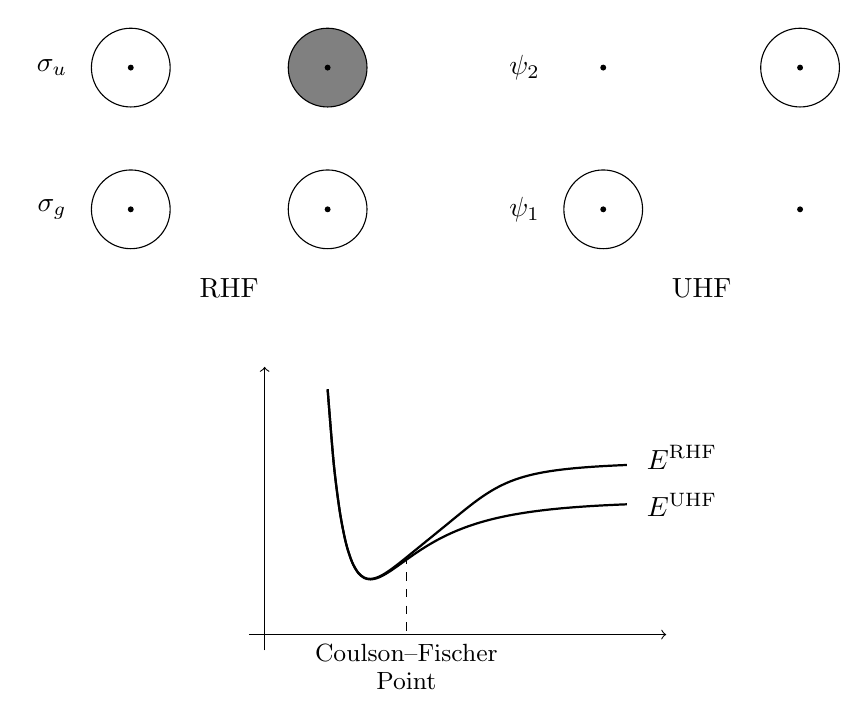
\begin{tikzpicture}
            \draw[fill=black] (0,0) circle (0.03);
            \draw[fill=black] (2.5,0) circle (0.03);
            \draw (0,0) circle (0.5);
            \draw (2.5,0) circle (0.5);
            \draw (0,1.8) circle (0.5);
            \draw[fill=gray] (2.5,1.8) circle (0.5);
            \draw[fill=black] (0,1.8) circle (0.03);
            \draw[fill=black] (2.5,1.8) circle (0.03);
            \node at (-1,0) {\(\sigma_g\)};
            \node at (-1,1.8) {\(\sigma_u\)};
            \node at (1.25,-1) {RHF};
            \draw[fill=black] (6,0) circle (0.03);
            \draw[fill=black] (8.5,0) circle (0.03);
            \draw (6,0) circle (0.5);
            \draw (8.5,1.8) circle (0.5);
            \draw[fill=black] (6,1.8) circle (0.03);
            \draw[fill=black] (8.5,1.8) circle (0.03);
            \node at (5,0) {\(\psi_1\)};
            \node at (5,1.8) {\(\psi_2\)};
            \node at (7.25,-1) {UHF};
            \draw[->] (1.5,-5.4)--(6.8,-5.4);
            \draw[->] (1.7,-5.6)--(1.7,-2);
            \draw[thick,domain=3.2:7, smooth, variable=\x,samples=50] plot ({\x-0.7}, {4*(((0.3*\x)^(-12))-((0.3*\x)^(-6)))-3.45+((1-2^(25-5*\x))/(4*(1+2^(25-5*\x))))});
            \draw[thick,domain=3.2:7, smooth, variable=\x,samples=50] plot ({\x-0.7}, {4*(((0.3*\x)^(-12))-((0.3*\x)^(-6)))-3.7});
            \node at (7,-3.15) {\(E^{\text{RHF}}\)};
            \node at (7,-3.75) {\(E^{\text{UHF}}\)};
            \draw[dashed] (3.5,-4.4)--(3.5,-5.4)node[below,align=center]{\small Coulson--Fischer \\[-2pt] \small Point};
        \end{tikzpicture}
        \caption{UHF allows \(\alpha\) and \(\beta\) spin electrons to take different spatial orbitals. This makes UHF significantly better than RHF when calculating dissociation.}
    \end{figure}

    We can see that the main advantage of the UHF wavefunction is its simplicity and also that since the alpha and beta orbitals may be different, alpha and beta electrons avoid one another and therefore said to be correlated. No such correlation is present in RHF wavefunctions.

    An objection to UHF theory is that the wavefunction is not an eigenfunction of \(\hat{S}^2\). The spin contamination may be measured from the expectation value of \(\hat{S}^2\)
    \begin{equation}
        \expval{\hat{S}^2}{\Phi}=M_S(M_S+1)+n^\beta-\sum_{i}^{\alpha}\sum_{j}^{\beta}(S_{ij}^{\alpha\beta})^2\,,
    \end{equation}
    where \(M_S\coloneqq\frac{1}{2}(n^\alpha-n^\beta)\) and \(S_{ij}^{\alpha\beta}=\braket{\phi_i^\alpha}{\phi_j^\beta}\).

    \newpage
    \section{Electron Correlation}
    The self-consistent field method is an independent electron approximation. This is understood by recognising that each orbital is an eigenfunction of the same Fock Hamiltonian. Further, the wavefunction only depends upon the absolute coordinate of each electron, and not on the distance between the electrons. The motion of the electrons is therefore not correlated. The difference between the SCF energy using a large basis set (the so-called Hartree--Fock energy) and the exact energy of the Schr\"{o}dinger Hamiltonian is called the correlation energy
    \begin{equation}
        E_{\text{corr}}=E_{\text{exact}}-E_{\text{RHF}}<0\,.
    \end{equation}
    Correlation energy is usually pretty significant, being approximately 0.04 Hartrees (\(100\unit{kJ}\unit{mol}^{-1}\)) for two electrons in a doubly occupied orbital. Therefore if a single bond is broken, this quantity is released. It is therefore important to be able to calculate the value of the correlation energy for a molecular system.

    A simple way forward is to introduce interelectronic distances \(r\equiv r_{ij}=\norm{\vb{r}_i-\vb{r}_j}\) into the wavefunction. We can see why this is a good idea. Consider two electrons of opposite spin moving in space. Noting that their reduced mass is \(m/2\) and denoting \(r\) as the distance between them, the Schr\"{o}dinger equation for their motion is
    \begin{equation}
        \left(-\laplacian+\frac{1}{r}\right)\psi=E\psi\,.
    \end{equation}
    Expanding the Laplacian in spherical polar coordinates yields
    \begin{equation}
        \left(-\pdv[2]{}{r}-\frac{2}{r}\pdv{}{r}+\frac{\hat{\vb{L}}^2}{r^2}+\frac{1}{r}\right)\psi=E\psi\,,
    \end{equation}
    where \(\hat{\vb{L}}\) is the angular momentum operator. We now want to find a series expansion solution for an \(\mathrm{s}\) orbital near \(r=0\), so that we can ignore the \(\hat{L}\) part. We write \(\psi(r)=a+br+\mathcal{O}(r^2)\), substitute in the equation and let the coefficient of \(r^{-1}\) be zero. This yields
    \begin{equation}
        \psi(r_{ij})=a\left(1+\frac{1}{2}r_{ij}+\mathcal{O}(r_{ij}^2)\right)\,.
    \end{equation}
    This expression demonstrates the reduction in probability as two electrons approach one another, although of course because the electrons have different spins, the wavefunction is not zero at coincidence. Thus we have shown that the exact wavefunction must contain terms which are linear in interelectronic distances.
    
    However, we cannot proceed this way because the matrix elements of wavefunctions would then involve \(3n\)-dimensional integrals, where \(n\) is the number of electrons. The main current way forward is to continue with the use of determinants. We can easily show that by taking a linear combination of determinants we can introduce the square of the interelectronic distances. Consider a four-determinant wavefunction of the He atom
    \begin{equation}
        \Psi=\sum_{I=1}^{4}c_I\antisymm(\phi_I^\alpha\phi_I^\beta)\,,
    \end{equation}
    where
    \begin{equation}
        c_1=1\,,\; c_2=c_3=c_4=c\,.
    \end{equation}
    \begin{equation}
        \phi_1=\exp(-2r)\,,
    \end{equation}
    \begin{equation}
        \phi_2=x\phi_1\,,\;\phi_3=y\phi_1\,,\;\phi_4=z\phi_1\,.
    \end{equation}
    \(\phi_1\) corresponds to the 1s orbital and \(\phi_2,\phi_3,\phi_4\) corresponds to the 2p\(_x\), 2p\(_y\) and 2p\(_z\) orbitals respectively. Hence these four determinants correspond to the four states shown in the figure below.

    \begin{figure}[ht!]
        \centering
        \begin{tikzpicture}
            \node at (-1.5,3) {\(I=\)};
            \node at (-1.5,0.5) {\(c_I=\)};
            \foreach \x in {1,2,3,4}{
                \node at (-3+3*\x,3) {\(\x\)};
                \draw (-2.75+3*\x,2)--(-3.25+3*\x,2);
                \draw (-2.75+3*\x,1.2)--(-3.25+3*\x,1.2);
                \draw (-3.95+3*\x,2)--(-3.45+3*\x,2);
                \draw (-2.05+3*\x,2)--(-2.55+3*\x,2);
                \draw[->] (-0.05,1)--(-0.05,1.4);
                \draw[<-] (0.05,1)--(0.05,1.4);
                \draw[->] (2.25,1.8)--(2.25,2.2);
                \draw[<-] (2.35,1.8)--(2.35,2.2);
                \draw[->] (5.95,1.8)--(5.95,2.2);
                \draw[<-] (6.05,1.8)--(6.05,2.2);
                \draw[->] (9.65,1.8)--(9.65,2.2);
                \draw[<-] (9.75,1.8)--(9.75,2.2);
                \node at (0,0.5) {\(1\)};
                \node at (3,0.5) {\(c\)};
                \node at (6,0.5) {\(c\)};
                \node at (9,0.5) {\(c\)};
            }
        \end{tikzpicture}
    \end{figure}

    Substitution yields
    \begin{equation}
        \Psi=\frac{1}{\sqrt{2}}(\alpha\beta-\beta\alpha)\e^{-2(r_1+r_2)}(1+c(x_1x_2+y_1y_2+z_1z_2))\,.
    \end{equation}
    The result follows by noting
    \begin{equation}
        x_1x_2+y_1y_2+z_1z_2=\vb{r}_1\cdot\vb{r}_2=\frac{1}{2}(r_1^2+r_2^2-r_{12}^2)\,.
    \end{equation}
    The second, third and fourth determinants in the above example are each double replacements of the first determinant, and thus we have seen that double replacement determinants introduce the square of the interelectronic distances, and therefore introduce electron correlation effects into the wavefunction in the form
    \begin{equation}
        \Psi\sim(1+r_{12}^2+\dots)\,.
    \end{equation}

    Note that there exist methods called \textit{explicitly correlated}, often denoted \(f_{12}\) or \(f(r_{12})\), which include \(r_{12}\) in linear order into the wavefunction, but they are beyond the scope of our course.
    \subsection{Full Configuration Interaction}
    The way forward is therefore to represent the wavefunction as a linear combination of many determinants. We now denote the Hartree--Fock determinant as \(\Phi_0\), and in general, we can make the excited determinant using the same set of orbitals.
    \begin{figure}[ht!]
        \centering
        \begin{tikzpicture}
            \node at (0,0) {\(\phi_1\)};
            \node at (0,1.2) {\(\phi_2\)};
            \draw (0.5,0)--(1.5,0);
            \draw (0.5,1.2)--(1.5,1.2);
            \draw[->] (0.95,-0.3)--(0.95,0.3);
            \draw[<-] (1.05,-0.3)--(1.05,0.3);
            \draw (2.5,0)--(3.5,0);
            \draw (2.5,1.2)--(3.5,1.2);
            \draw[->] (2.95,0.9)--(2.95,1.5);
            \draw[<-] (3.05,0.9)--(3.05,1.5);
            \node at (1,-0.7) {\(\Phi_I\)};
            \node at (3,-0.7) {\(\Phi_J\)};
        \end{tikzpicture}
    \end{figure}

    Note that by the orthogonality of orbitals, we have
    \begin{equation}
        \bracket{\Phi_I}{\Phi_J}=\delta_{IJ}\,.
    \end{equation}
    In \textit{configuration interaction} (CI), we write the wavefunction as
    \begin{equation}
        \Psi=\sum_{I}c_I\Phi_I\,.
    \end{equation} 
    The CI coefficients \(c_I\) and the energy \(E\) are found by solving the secular equations
    \begin{equation}
        \sum_{J}\mel{\Phi_I}{\hat{H}-E}{\Phi_J}c_J=0\,.
    \end{equation}
    If one includes all possible determinants then this is called the \textit{full configuration interaction} (FCI) method and it gives the best possible solution to the Schr\"{o}dinger equation in the finite basis set we are using. However it is impractical for all but the tiniest system due to the exponentially large size of the matrix we have to diagonalise. Consider a system of \(m\) spatial orbitals and \(2n\) electrons. The number of determinants we need to include is
    \begin{equation}
        \begin{pmatrix}
            2m \\ 2n
        \end{pmatrix}=\frac{(2m)!}{(2n)!(2m-2n)!}=\mathcal{O}(\e^{am})\,.
    \end{equation}
    \begin{ex}
        \textit{Determine the symmetries of the ground and excited states in an FCI calculation for a minimal basis H\(_2\) molecule.}

        \begin{figure}[ht!]
            \centering
            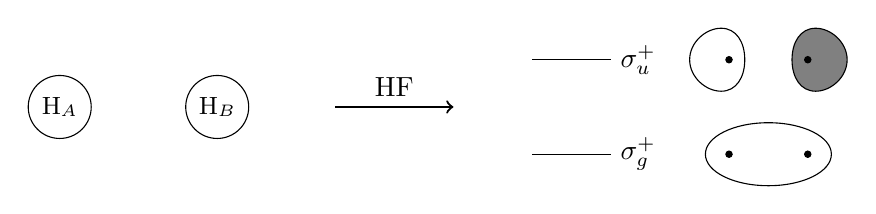
\begin{tikzpicture}
                \draw (0,0) circle (0.4);
                \node at (0,0) {\small H\(_A\)};
                \draw (2,0) circle (0.4);
                \node at (2,0) {\small H\(_B\)};
                \draw[thick,->] (3.5,0)--node[above]{HF}(5,0);
                \draw (6,-0.6)--(7,-0.6) node[right]{\(\sigma_g^+\)};
                \draw (6,0.6)--(7,0.6) node[right]{\(\sigma_u^+\)};
                \draw[fill=black] (8.5,-0.6) circle (0.04);
                \draw[fill=black] (9.5,-0.6) circle (0.04);
                \draw plot [smooth cycle, tension=1] coordinates { (8.2,-0.6) (9,-1) (9.8,-0.6) (9,-0.2) };
                \draw plot [smooth cycle, tension=1] coordinates { (8,0.6) (8.4,1) (8.7,0.6) (8.4,0.2) };
                \draw[fill=gray] plot [smooth cycle, tension=1] coordinates { (10,0.6) (9.6,1) (9.3,0.6) (9.6,0.2) };
                \draw[fill=black] (8.5,0.6) circle (0.04);
                \draw[fill=black] (9.5,0.6) circle (0.04);
            \end{tikzpicture}
        \end{figure}

        The number of determinants is
        \begin{equation}
            \begin{pmatrix}
                \# \text{ spin-orbitals} \\ \#\, e^-
            \end{pmatrix}=\begin{pmatrix}
                4 \\ 2
            \end{pmatrix}=6\,.
        \end{equation}
        \begin{figure}[ht!]
            \centering
            \begin{tikzpicture}
                \node at (0,0) {\(\sigma_g^+\)};
                \node at (0,1.4) {\(\sigma_u^+\)};
                \foreach \x in {1,...,6}{
                    \draw (2*\x-0.8,0)--(2*\x,0);
                    \draw (2*\x-0.8,1.4)--(2*\x,1.4);
                }
                \draw[->] (1.55,-0.3)--(1.55,0.3);
                \draw[<-] (1.65,-0.3)--(1.65,0.3);
                \draw[->] (3.6,-0.3)--(3.6,0.3);
                \draw[<-] (3.6,1.1)--(3.6,1.7);
                \draw[<-] (5.6,-0.3)--(5.6,0.3);
                \draw[->] (5.6,1.1)--(5.6,1.7);
                \draw[->] (7.55,1.1)--(7.55,1.7);
                \draw[<-] (7.65,1.1)--(7.65,1.7);
                \draw[->] (9.6,-0.3)--(9.6,0.3);
                \draw[->] (9.6,1.1)--(9.6,1.7);
                \draw[<-] (11.6,-0.3)--(11.6,0.3);
                \draw[<-] (11.6,1.1)--(11.6,1.7);
                \node at (0,-0.8) {symmetry};
                \node at (1.6,-0.8) {\(^1\Sigma_g^+\)};
                \draw [decorate,decoration={brace,amplitude=5pt,mirror}] (3.2,-0.4) -- (6,-0.4) node[midway,yshift=-1em]{\(^1\Sigma_u^+ \oplus {^3\Sigma_u^+}\)};
                \node at (7.6,-0.8) {\(^1\Sigma_g^+\)};
                \node at (10.6,-0.8) {\(^3\Sigma_u^+\)};
                \node at (4,-1.2) {\scriptsize \(M_S=0\)};
                \node at (5.2,-1.2) {\scriptsize \(M_S=0\)};
                \node at (9.6,-1.2) {\scriptsize \(M_S=1\)};
                \node at (11.6,-1.2) {\scriptsize \(M_S=-1\)};
            \end{tikzpicture}
        \end{figure}
    \end{ex}
    \subsection{Configuration Interaction with Singles and Doubles}
    The way forward is therefore to represent the wavefunction as a linear combination of many determinants, especially including all single and double replacements of the dominant SCF determinants to give \textit{configuration interaction with singles and doubles} (CISD). In practice it is found that the CI method is very slowly convergent, needing very large basis sets to generate a large number of virtual orbitals to use in the double replacement determinants. We can understand this: we have shown that the wavefunction requires terms linear in the interelectronic distance, but that CI only introduces the square of the interelectronic distance. It will then clearly take the CI wavefunction to involve many terms to approximate the true wavefunction. Even so, this is the only practical way forward. We have seen that the matrix element of the above secular equation can be evaluated in terms of one and two electron integrals. Almost all correlated wavefunction calculations are based on linear combination of determinants.

    \begin{figure}[ht!]
        \centering
        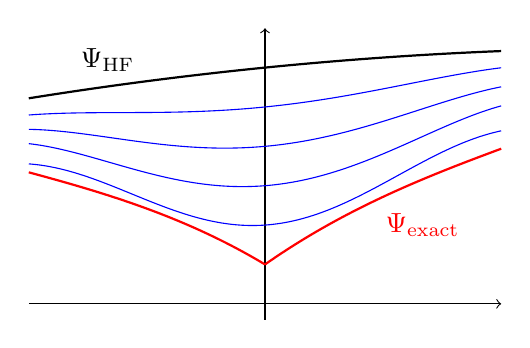
\begin{tikzpicture}
            \draw[->] (-3,0)--(3,0);
            \draw[->] (0,-0.2)--(0,3.5);
            \draw[red,thick,domain=0:3, smooth, variable=\x,samples=50] plot ({\x}, {0.5+0.7*\x-0.1*\x^2+0.01*\x^3});
            \draw[red,thick,domain=-3:0, smooth, variable=\x,samples=50] plot ({\x}, {0.5-0.6*\x-0.1*\x*\x-0.01*\x^3});
            \node[red] at (2,1) {\(\Psi_{\text{exact}}\)};
            \draw[thick,domain=-3:3, smooth, variable=\x,samples=50] plot ({\x}, {3+0.1*\x-0.01*\x*\x});
            \draw[blue,domain=-3:3, smooth, variable=\x,samples=50] plot ({\x}, {2.5+0.1*\x+0.04*\x*\x-0.002*(\x)^4});
            \draw[blue,domain=-3:3, smooth, variable=\x,samples=50] plot ({\x}, {2+0.09*\x+0.09*\x*\x-0.004*(\x)^4});
            \draw[blue,domain=-3:3, smooth, variable=\x,samples=50] plot ({\x}, {1.5+0.08*\x+0.14*\x*\x-0.006*(\x)^4});
            \draw[blue,domain=-3:3, smooth, variable=\x,samples=50] plot ({\x}, {1+0.07*\x+0.22*\x*\x-0.015*(\x)^4+0.0003*(\x)^6});
            \node at (-2,3.1) {\(\Psi_{\text{HF}}\)};
        \end{tikzpicture}
        \caption{Increasing the size of basis set generates more virtual orbitals that allow us to include more terms in configuration interaction.}
    \end{figure}

    The introduction of higher angular momentum in basis results in better cusps. It can be shown from partial wave expansion that the truncation error is of the order
    \begin{equation}
        \Delta E\sim c(l_{\text{trunc}}+1)^{-3}\,.
    \end{equation}
    We can extrapolate energies with increasing basis set.
    \subsection{Size Consistency}
    There is a further difficulty with straightforward truncated CI called the problem of \textit{size consistency}. A method is said to be \textit{size consistent} if the energy of a composite system A\(-\)B at infinite separation is the same as the energy of A plus the energy of B evaluated separately.

    \begin{figure}[ht!]
        \centering
        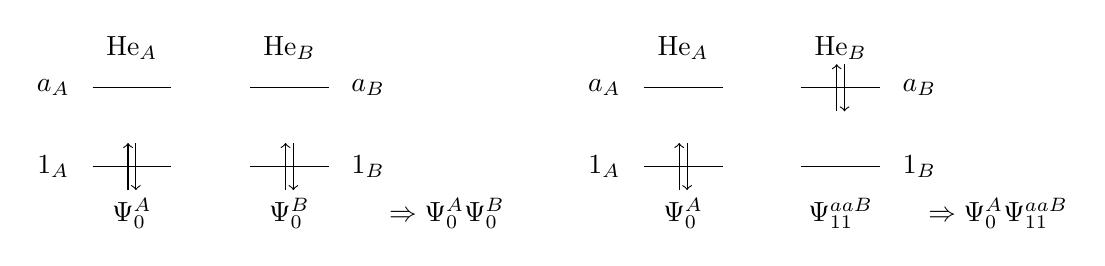
\begin{tikzpicture}
            \node at (-0.5,0) {\(1_A\)};
            \node at (-0.5,1) {\(a_A\)};
            \draw (0,0)--(1,0);
            \draw (0,1)--(1,1);
            \node at (0.5,1.5) {He\(_{A}\)};
            \node at (0.5,-0.6) {\(\Psi_{0}^{A}\)};
            \draw[->] (0.45,-0.3)--(0.45,0.3);
            \draw[<-] (0.55,-0.3)--(0.55,0.3);
            \draw (2,0)--(3,0);
            \draw (2,1)--(3,1);
            \node at (2.5,1.5) {He\(_{B}\)};
            \node at (2.5,-0.6) {\(\Psi_{0}^{B}\)};
            \node at (3.5,0) {\(1_B\)};
            \node at (3.5,1) {\(a_B\)};
            \draw[->] (2.45,-0.3)--(2.45,0.3);
            \draw[<-] (2.55,-0.3)--(2.55,0.3);
            \node at (4.5,-0.6) {\(\Rightarrow \Psi_{0}^{A}\Psi_{0}^{B}\)};
            \begin{scope}[shift={(7,0)}]
                \node at (-0.5,0) {\(1_A\)};
                \node at (-0.5,1) {\(a_A\)};
                \draw (0,0)--(1,0);
                \draw (0,1)--(1,1);
                \node at (0.5,1.5) {He\(_{A}\)};
                \node at (0.5,-0.6) {\(\Psi_{0}^{A}\)};
                \draw[->] (0.45,-0.3)--(0.45,0.3);
                \draw[<-] (0.55,-0.3)--(0.55,0.3);
                \draw (2,0)--(3,0);
                \draw (2,1)--(3,1);
                \node at (2.5,1.5) {He\(_{B}\)};
                \node at (2.5,-0.6) {\(\Psi_{11}^{aaB}\)};
                \node at (3.5,0) {\(1_B\)};
                \node at (3.5,1) {\(a_B\)};
                \draw[->] (2.45,0.7)--(2.45,1.3);
                \draw[<-] (2.55,0.7)--(2.55,1.3);
                \node at (4.5,-0.6) {\(\Rightarrow \Psi_{0}^{A}\Psi_{11}^{aaB}\)};
            \end{scope}
        \end{tikzpicture}
        \caption{The ground state and an excited configuration of the He\(_2\) system.}
    \end{figure}

    Consider a wavefunction for He involving one double replacement
    \begin{equation}
        \Psi=\Psi_0+c\Psi_{11}^{aa}\,.
    \end{equation}
    For two such He atoms represented by such a wavefunction a long way apart, the correct combined wavefunction is
    \begin{equation}
        (\Psi_{0}^{A}+c\Psi_{11}^{aaA})(\Psi_{0}^{B}+c\Psi_{11}^{aaB})=\Psi_{0}^{A}\Psi_{0}^{B}+c(\Psi_{11}^{aaA}\Psi_{0}^{B}+\Psi_{11}^{aaB}\Psi_{0}^{A})+c^2\Psi_{11}^{aaA}\Psi_{11}^{aaB}\,.
    \end{equation}
    This wavefunction involves fourfold replacement of the reference wavefunction. Thus if the CI of the composite \(\mathrm{He_2}\) system is restricted to double replacements, the last term is removed, and then the wavefunction and its energy will not correspond to that of two separated He atoms. In practice it is very difficult to include all possible determinants in a full-CI calculation and therefore limited CI calculations suffer from this deficiency which is found to be significant numerically. On the other hand methods based on perturbation theory are size consistent as we shall see later.

    There are two types of electron correlation effects, dynamic and non-dynamic. \textit{Dynamic correlation} is like that met in the He atom, essentially arising from the reduction in probability of two electrons coming together. It is said to be short-range correlation. Electrons want to be further apart, and thus the electron repulsion contribution to the total energy is lowered. \textit{Non-dynamic correlation} is best explained through CI. We have seen that to describe the dissociation of H\(_{2}\) correctly, it is necessary to include the determinant \(\antisymm(\sigma_u^2)\) in addition to the determinant \(\antisymm(\sigma_g^2)\), and at infinite separation these two determinants are of equal weight because they are degenerate.\footnote{See course \textit{A4: Theoretical Techniques}.} Non-dynamic electron correlation is therefore long range, and is introduced in CI by including those determinants which are essential to ensure correct dissociation. Such determinants are approximations to low-lying electronic states.

    \subsection{M\o ller--Plesset Theory}
    This is the simplest way to include the effects of electron correlation. It is an example of second order Rayleigh--Schr\"{o}dinger perturbation theory.\footnote{We will only introduce the non-degenerate time independent perturbation theory. See more details, including a discussion on degenerate perturbation theory and time dependent perturbation theory in course \textit{C7: Further Quantum Mechanics}. If you are interested in some mathematical details, see my notes on Mathematical Tripos Part II: \textit{Principles of Quantum Mechanics}.}
    \begin{thm}[Rayleigh--Schr\"{o}dinger perturbation theory]
        Suppose we have an exactly solvable reference eigenvalue problem
        \begin{equation}
            \hat{H}^{(0)}\Psi_i^{(0)}=E_i^{(0)}\Psi_i^{(0)}\,,
        \end{equation}
        and we are interested in solving a related eigenvalue problem
        \begin{equation}
            \hat{H}\Psi_i=E_i\Psi_i\,,
        \end{equation}
        where
        \begin{equation}
            \hat{H}=\hat{H}^{(0)}+\hat{H}^{(1)}
        \end{equation}
        for some small \textit{perturbation} \(\hat{H}^{(1)}\). Then if the eigenstate \(\Psi_i^{(0)}\) of \(\hat{H}^{(0)}\) is non-degenerate,
        \begin{equation}
            E_i^{(1)}=\expval{\hat{H}^{(1)}}{\Psi_i^{(0)}}\,,
        \end{equation}
        \begin{equation}
            \Psi_i^{(1)}=\sum_{j\ne i}\frac{\mel{\Psi_j^{(0)}}{\hat{H}^{(1)}}{\Psi_i^{(0)}}}{E_{i}^{(0)}-E_j^{(0)}}\Psi_j^{(0)}\,,
        \end{equation}
        \begin{equation}
            E_i^{(2)}=\mel{\Psi_i^{(0)}}{\hat{H}^{(1)}}{\Psi_{i}^{(1)}}\,.
        \end{equation}
    \end{thm}
    \begin{proof}
        Let the Hamiltonian depend smoothly on a parameter \(\lambda\)
        \begin{equation}
            \hat{H}(\lambda)=H^{(0)}+\lambda\hat{H}^{(1)}\,.
        \end{equation}
        Then \(\hat{H}(1)\) is the question we are interested in. The key is to assume that the eigenfunctions and eigenvectors of \(\hat{H}(\lambda)\) are also analytic on the parameter \(\lambda\), so that we can express them as a series expansion
        \begin{align}
            \Psi_i&=\Psi_i^{(0)}+\lambda\Psi_i^{(1)}+\lambda^2\Psi_i^{(2)}+\mathcal{O}(\lambda^3)\,, \\
            E_i&=E_i^{(0)}+\lambda E_i^{(1)}+\lambda^2 E_i^{(2)}+\mathcal{O}(\lambda^3)\,,
        \end{align}
        such that
        \begin{equation}
            \hat{H}\Psi_i=E\Psi_i
        \end{equation}
        with the conventional \textit{intermediate normalisation}. Then
        \begin{equation}
            \braket{\Psi_i^{(0)}}{\Psi_i}=1\quad\Rightarrow\quad\braket{\Psi_i^{(0)}}{\Psi_i^{(n)}}=0
        \end{equation}
        for all \(n\ne 0\). Then we can expand \(\hat{H}\Psi_i=E\Psi_i\) to get
        \begin{align}
            (\hat{H}^{(0)}+\lambda\hat{H}^{(1)})&(\Psi_i^{(0)}+\lambda\Psi_i^{(1)}+\lambda^2\Psi_i^{(2)}+\dots) \notag \\
            &=(E_i^{(0)}+\lambda E_i^{(1)}+\lambda^2 E_i^{(2)}+\dots)(\Psi_i^{(0)}+\lambda\Psi_i^{(1)}+\lambda^2\Psi_i^{(2)}+\dots)\,,
        \end{align}
        which holds true for all \(\lambda\). Hence, we gather terms in the same order of \(\lambda\) and get
        \begin{align}
            \lambda^0:&& \hat{H}^{(0)}\Psi_i^{(0)}&=E_i^{(0)}\Psi_i^{(0)}\\
            \lambda^1:&& \hat{H}^{(1)}\Psi_i^{(0)}+\hat{H}^{(0)}\Psi_i^{(1)}&=E_i^{(1)}\Psi_i^{(0)}+E_i^{(0)}\Psi_i^{(1)}\\
            \lambda^2:&& \hat{H}^{(1)}\Psi_i^{(1)}+\hat{H}^{(0)}\Psi_i^{(2)}&=E_i^{(0)}\Psi_i^{(2)}+E_i^{(1)}\Psi_i^{(1)}+E_i^{(2)}\Psi_i^{(0)}\\
            && &\dots \notag
        \end{align}
        To extract \(E^{(1)}\), we act \(\bra{\Psi_i^{(0)}}\) to the terms in the order of \(\lambda^1\) to get
        \begin{equation}
            \expval{\hat{H}^{(1)}}{\Psi_i^{(0)}}+\underbrace{\mel{\Psi_i^{(0)}}{\hat{H}^{(0)}}{\Psi_i^{(1)}}}_{=\braket{E_i^{(0)}\Psi_i^{(0)}}{\Psi_i^{(1)}}=0}=E_i^{(1)}\underbrace{\braket{\Psi_i^{(0)}}{\Psi_i^{(0)}}}_{=1}+E_i^{(0)}\underbrace{\braket{\Psi_i^{(0)}}{\Psi_i^{(1)}}}_{=0}\,,
        \end{equation}
        which rearranges to give
        \begin{equation}
            E_i^{(1)}=\expval{\hat{H}^{(1)}}{\Psi_i^{(0)}}\,.
        \end{equation}
        Next, to work out \(\Psi_i^{(1)}\), we act \(\bra{\Psi_j^{(0)}}\) to the terms of order \(\lambda^1\) to get
        \begin{equation}
            \mel{\Psi_j^{(0)}}{\hat{H}^{(1)}}{\Psi_i^{(0)}}+\underbrace{\mel{\Psi_j^{(0)}}{\hat{H}^{(0)}}{\Psi_i^{(1)}}}_{=\braket{E_j^{(0)}\Psi_j^{(0)}}{\Psi_i^{(1)}}}=E_i^{(1)}\underbrace{\braket{\Psi_j^{(0)}}{\Psi_i^{(0)}}}_{=\delta_{ij}}+E_i^{(0)}\braket{\Psi_j^{(0)}}{\Psi_i^{(1)}}\,,
        \end{equation}
        \begin{equation}
            \mel{\Psi_j^{(0)}}{\hat{H}^{(1)}}{\Psi_i^{(0)}}=(-E_j^{(0)}+E_i^{(0)})\braket{\Psi_j^{(0)}}{\Psi_i^{(1)}}\,.
        \end{equation}
        Since \(\{\Psi_j^{(0)}\}\) is a complete orthonormal basis set and \(\braket{\Psi_i^{(0)}}{\Psi_i^{(1)}}=0\), we have
        \begin{equation}
            \Psi_i^{(1)}=\sum_{j}\ket{\Psi_j^{(0)}}\braket{\Psi_j^{(0)}}{\Psi_i^{(1)}}=\sum_{j\ne i}\frac{\mel{\Psi_j^{(0)}}{\hat{H}^{(1)}}{\Psi_i^{(0)}}}{E_{i}^{(0)}-E_j^{(0)}}\Psi_j^{(0)}\,.
        \end{equation}
        Similarly, by acting \(\ket{\Psi_i^{(0)}}\) on the \(\lambda^2\) terms, we get
        \begin{equation}
            E_i^{(2)}=\mel{\Psi_i^{(0)}}{\hat{H}^{(1)}}{\Psi_{i}^{(1)}}
        \end{equation}
        \textit{etc.}\qed
    \end{proof}

    Our system of interest is clearly the Schr\"{o}dinger Hamiltonian \(\hat{H}\), and we need to find a reference Hamiltonian that has known eigenstates and eigenvalues. Having just derived the Hartree--Fock theory, the sum of the Fock operators is obviously a good choice. Let
    \begin{equation}
        \hat{H}^{(0)}=\sum_{i=1}^{n}\hat{F}(i)\,,
    \end{equation}
    \begin{equation}
        \hat{H}^{(1)}=\hat{H}-\hat{H}^{(0)}\,.
    \end{equation}
    In the restricted space defined by the basis set, the orbitals are eigenfunctions of the Fock operators
    \begin{equation}
        \hat{F}\phi_p=\epsilon_p\phi_p\,.
    \end{equation}
    It follows that in zeroth order, the eigenstates of \(\hat{H}^{(0)}\) are the Slater determinants made out of \(n\) of the \(m\) spin-orbitals, denoted \(\Phi_I\coloneqq\antisymm(\phi_{I_1}\dots\phi_{I_n})\), such that
    \begin{align}
        \hat{H}^{(0)}\Phi_I&=E_I^{(0)}\Phi_I\,, \\
        E_I^{(0)}&=\sum_{i=1}^{n}\epsilon_{I_i}\,.
    \end{align}
    Particularly, the ground state
    \begin{align}
        \hat{H}^{(0)}\Phi_0^{(0)}&=E_0^{(0)}\Phi_0^{(0)}\,,\\
        E_0^{(0)}&=\sum_{i=1}^{n}\epsilon_i\,.
    \end{align}
    This method is the \textit{M\o ller--Plesset theory}, MP\(n\), where \(n\) labels the order of perturbation we consider.

    The zeroth order energy is simply the sum of the orbital energies, which is a very poor estimate of the total energy because it involves double counting. Now from perturbation theory, the first order correction is
    \begin{equation}
        E_I^{(1)}=\expval{\hat{H}^{(1)}}{\Phi_I^{(0)}}
    \end{equation}
    and hence to the first order, the total ground state energy is
    \begin{equation}
        E_0^{(0)}+E_0^{(1)}=\expval{\hat{H}}{\Phi_0^{(0)}}=E_{\text{HF}}\,,
    \end{equation}
    which is exactly the Hartree--Fock SCF energy.

    Next, we want to calculate the second order energy correction, but first we need the ground state wavefunction corrected to the first order. By Rayleigh--Schr\"{o}dinger perturbation theory, it can be expanded in the orthonormal set \(\{\Phi_I\}\), which are the eigenstates of \(\hat{H}^{(0)}\), as
    \begin{equation}
        \Phi^{(1)}=\sum_{I\ne 0}C_I\Phi_I\,,
    \end{equation}
    where
    \begin{equation}
        C_I=-\frac{\mel{\Phi_I}{\hat{H}^{(1)}}{\Phi_0^{(0)}}}{H_{II}^{(0)}-E_0^{(0)}}\,.
    \end{equation}
    Replacement of \(\hat{H}^{(1)}\) by \(\hat{H}-\hat{H}^{(0)}\) yields
    \begin{equation}\label{MP2_wavefunction_coefficients}
        C_I=-\frac{\mel{\Phi_I}{\hat{H}}{\Phi_0^{(0)}}}{H_{II}^{(0)}-E_0^{(0)}}\,.
    \end{equation}
    Now we consider the various possibilities for \(\Phi_I\).
    \begin{enumerate}[topsep=0pt,label=(\roman*)]
        \item Single replacement determinants \(\Phi_{i}^{a}\).
        
        By \cref{replacement_matrix_elements} and (\ref{closed_shell_SCF_conditions}), we get
        \begin{equation}
            \mel{\Phi_{i}^{a}}{\hat{H}}{\Phi_0^{(0)}}=F_{ai}=0\,.
        \end{equation}
        This is known as Brillouin's theorem.
        \item Double replacement determinants \(\Phi_{ij}^{ab}\).
        
        By \cref{replacement_matrix_elements},
        \begin{equation}
            \mel{\Phi_{ij}^{ab}}{\hat{H}}{\Phi_0^{(0)}}=\bracket{ai}{bj}-\bracket{aj}{bi}\,.
        \end{equation}
        \item Triple and higher replacement determinants \(\Phi_{ijk\dots}^{abc\dots}\).
        \begin{equation}
            \mel{\Phi_{ijk\dots}^{abc\dots}}{\hat{H}}{\Phi_0^{(0)}}=0
        \end{equation}
        because \(\hat{H}\) has no three electron operators.
    \end{enumerate}
    
    Thus the only coefficients in (\ref{MP2_wavefunction_coefficients}) that are non-vanishing are those for double replacements. This shouldn't be surprising following our CI discussion. For a particular \(\Phi_{ij}^{ab}\) the denominator is
    \begin{equation}
        H_{II}^{(0)}-E_0^{(0)}=\epsilon_a+\epsilon_b-\epsilon_i-\epsilon_j\,,
    \end{equation}
    and note that \(\Phi_{ij}^{ab}\), \(-\Phi_{ji}^{ab}\), \(-\Phi_{ij}^{ba}\) and \(\Phi_{ji}^{ba}\) are the same, the second order ground state energy correction hence takes the form
    \begin{align}
        E_0^{(2)}&=-\sum_{I}\frac{\abs{\mel{\Phi_I}{\hat{H}}{\Phi^{(0)}_0}}^2}{H_{II}^{(0)}-E_0^{(0)}}\notag\\
        &=-\frac{1}{4}\sum_{i,j=1}^{n}\sum_{a,b=n+1}^{m}\frac{[\bracket{ia}{jb}-\bracket{ib}{ja}]^2}{\epsilon_a+\epsilon_b-\epsilon_i-\epsilon_j} \label{MP2_energy_correction}\notag\\
        &\eqqcolon\sum_{ij}\epsilon_{ij}\,,
    \end{align}
    where \(\epsilon_{ij}\) may be interpreted as the correlation energy of a pair of electrons.

    For a closed-shell system \(\Phi_0=\antisymm(\phi_1^\alpha\phi_1^\beta\phi_2^\alpha\phi_2^\beta\dots\phi_n^\alpha\phi_n^\beta)\) with \(2n\) electrons, we can work out the terms vanishing due to spins in (\ref{MP2_energy_correction}). Consider the possible spin combinations for a particular set of spatial orbital \(i,j,a,b\):
    \begin{table}[ht!]
        \centering
        \begin{tabular}{ccccccc}
            \toprule
            Spatial & \(i\) & \(a\) & \(j\) & \(b\) & \(\bracket{ia}{jb}\) & \(\bracket{ib}{ja}\) \\ \midrule
            \multirow{6}{*}{Spin} & \(\alpha\) & \(\alpha\) & \(\alpha\) & \(\alpha\) & \tikzcmark & \tikzcmark \\
            ~ & \(\beta\) & \(\beta\) & \(\beta\) & \(\beta\) & \tikzcmark & \tikzcmark \\
            ~ & \(\alpha\) & \(\alpha\) & \(\beta\) & \(\beta\) & \tikzcmark & \tikzxmark \\
            ~ & \(\beta\) & \(\beta\) & \(\alpha\) & \(\alpha\) & \tikzcmark & \tikzxmark \\
            ~ & \(\alpha\) & \(\beta\) & \(\beta\) & \(\alpha\) & \tikzxmark & \tikzcmark \\
            ~ & \(\beta\) & \(\alpha\) & \(\alpha\) & \(\beta\) & \tikzxmark & \tikzcmark \\ \bottomrule
        \end{tabular}
    \end{table}\\
    and all other combinations of spins vanish. Summing these up gives
    \begin{align}
        E_0^{(2)}&=-\frac{1}{4}\sum_{i,j=1}^{n}\sum_{a,b=n+1}^{m}\frac{4\bracket{ia}{jb}^2+4\bracket{ib}{ja}^2-4\bracket{ia}{jb}\bracket{ib}{ja}}{\epsilon_a+\epsilon_b-\epsilon_i-\epsilon_j}\,.
    \end{align}
    Since \(\sum_{ijab}\bracket{ib}{ja}^2=\sum_{ijab}\bracket{ia}{jb}^2\), we can further simplify this to get
    \begin{equation}
        E_0^{(2)}=-\sum_{i,j,a,b}\frac{\bracket{ia}{jb}[2\bracket{ia}{jb}-\bracket{ib}{ja}]}{\epsilon_a+\epsilon_b-\epsilon_i-\epsilon_j}\,.
    \end{equation}
    \begin{equation}
        E_{\text{MP2}}=E_0^{(0)}+E_0^{(1)}+E_0^{(2)}=E_{\text{HF}}+E_0^{(2)}\,.
    \end{equation}
    \subsubsection{Size Consistency}
    Finally we need to explain why MP2 is a size consistent energy expression. We will assert, without proof, the following lemma.
    \begin{lem}
        The M\o ller--Plesset energy is invariant to occupied-occupied and virtual-virtual orbitals unitary rotations of degenerate orbitals.
    \end{lem}
    \begin{rem}
        This is analogous to \cref{energy_invariance_unitary_rotation}.
    \end{rem}
    Consider two He atoms, each with 1s and 2s basis. At infinity, they give a pair of degenerate \(1\sigma_g\), \(1\sigma_u\) orbitals
    \begin{align}
        \ket{1\sigma_g}&=\frac{\ket{1s_A}+\ket{1s_B}}{\sqrt{2}}\,,\\
        \ket{1\sigma_u}&=\frac{\ket{1s_A}-\ket{1s_B}}{\sqrt{2}}\,.
    \end{align}
    By the above lemma, they can be localised on each atom.
    \begin{figure}
        \centering
        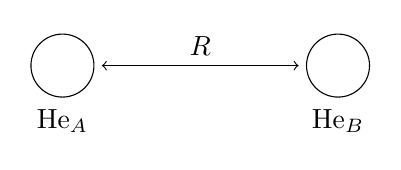
\begin{tikzpicture}
            \draw (0,0) circle (0.4);
            \draw (3.5,0) circle (0.4);
            \node at (0,-0.7) {He\(_A\)};
            \node at (3.5,-0.7) {He\(_B\)};
            \draw[<->] (0.5,0)-- node[above]{\(R\)}(3,0);
        \end{tikzpicture}
    \end{figure}
    \begin{figure}
        \centering
        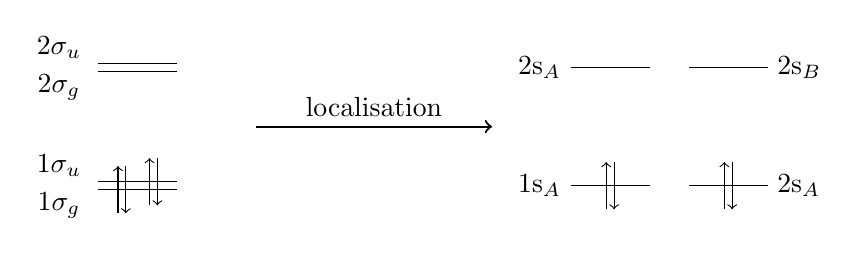
\begin{tikzpicture}
            \draw (-0.5,-0.05)--(0.5,-0.05);
            \draw (-0.5,0.05)--(0.5,0.05);
            \draw (-0.5,1.45)--(0.5,1.45);
            \draw (-0.5,1.55)--(0.5,1.55);
            \node at (-1,-0.25) {\(1\sigma_g\)};
            \node at (-1,0.25) {\(1\sigma_u\)};
            \node at (-1,1.25) {\(2\sigma_g\)};
            \node at (-1,1.75) {\(2\sigma_u\)};
            \draw[->] (-0.25,-0.35)--(-0.25,0.25);
            \draw[<-] (-0.15,-0.35)--(-0.15,0.25);
            \draw[->] (0.15,-0.25)--(0.15,0.35);
            \draw[<-] (0.25,-0.25)--(0.25,0.35);

            \draw[->,thick] (1.5,0.75)--node[above]{localisation}(4.5,0.75);

            \draw (5.5,0)node[left]{1s\(_A\)}--(6.5,0);
            \draw (5.5,1.5)node[left]{2s\(_A\)}--(6.5,1.5);
            \draw (7,0)--(8,0)node[right]{2s\(_A\)};
            \draw (7,1.5)--(8,1.5)node[right]{2s\(_B\)};
            \draw[->] (5.95,-0.3)--(5.95,0.3);
            \draw[<-] (6.05,-0.3)--(6.05,0.3);
            \draw[->] (7.45,-0.3)--(7.45,0.3);
            \draw[<-] (7.55,-0.3)--(7.55,0.3);
        \end{tikzpicture}
        \caption{A localisation of a He\(_2\) system that shows that MP2 is size consistent.}
    \end{figure}
    Thus a term in the MP2 energy expression \([\bracket{ai}{bj}-\bracket{aj}{bi}](\epsilon_a+\epsilon_b-\epsilon_i-\epsilon_j)^{-1}\) is only non-zero if the orbitals \(\phi_a\), \(\phi_b\), \(\phi_i\) and \(\phi_j\) are all on the same atom, in which case the term will be a part of the energy of the separate system A or B. If the orbitals are not all on A, or all on B, then the two electron integrals will be zero by zero overlap. Thus the sum of the separate energies of A and B is obtained. If we consider a large molecule, then the MP2 method will obtain the pair energies for all pairs of electrons, and thus there will be no degradation with system size.

    On the other hand for CI, the percentage of the wavefunction accounted for by the reference configuration, single excitation and double excitations rapidly decreases as the number of electrons increases because of the increasingly large proportion of all the other excitation, i.e.
    \begin{equation}
        \braket{\Psi_{\text{CISD}}}{\Psi_{\text{FCI}}}\downarrow\text{ as }n_{e^-}\uparrow\,.
    \end{equation}
    Thus CI cannot be used for the study of large molecules.

    \subsubsection{Higher Orders of Perturbation Theory}
    The M\o ller--Plesset perturbation theory can be extended to include not only the second, but also the third and fourth order perturbation, named MP2, MP3, MP4 \textit{etc.} MP2 is always useful, because for the ground state the energy correction is always negative (clear by the form of (\ref{MP2_energy_correction})) as it picks up electron corrections. However, it is not guaranteed that the MP2 energy is higher than the true ground state energy since the correction term
    \begin{equation}
        E_0^{(2)}=\mel{\Phi_0^{(0)}}{\hat{H}^{(1)}}{\Phi_0^{(1)}}
    \end{equation}  
    is not the expectation value of \(\hat{H}\) for a single state, so the variational principles do not apply.

    It has been argued that the higher orders, especially MP4, will give greater accuracy, because they introduce higher order excitations (e.g. MP4 introduces three- and four- replacements). However, it has been demonstrated, by using larger basis sets in full-CI calculations, in many cases that the perturbation series for \(\hat{H}(\lambda)=\hat{H}^{(0)}+\lambda\hat{H}^{(1)}\) has singularities inside \(\abs{\lambda}=1\), and thus the series is not convergent for \(\lambda=1\). For example, it is explicitly shown that for Ne, the ground state and first excited state of \(\hat{H}(\lambda)\) become degenerate when \(\lambda=-0.82\). This problem is more severe if the electron correlation is strong so that the perturbation is large. For example, if we add a quartic potential perturbation to a harmonic oscillator's quadratic potential, then the radius of convergence of the perturbation energy will have a radius of convergence of zero.

    \begin{figure}
        \centering
        \include{Perturbation.tex}
        \vskip -20 pt
        \caption{Dissociation of \(\mathrm{H_2}\) using different orders of M\o ller--Plesset perturbation theory with cc-pVTZ basis. The result of full-CI is also included, which can be seen as the correct answer. We see that a higher order of perturbation does not necessarily give a better answer, especially when the perturbation is large. In the \(r\to\infty\) limit, the correlation is so large that the \(1\sigma_g^+\) and \(1\sigma_u^+\) orbitals of \(\mathrm{H_2}\) become degenerate, so the MP2 energy diverges to infinity. This is also the case for higher-order perturbations. (In fact in this case CCSD(T) will also break down for molecules apart from hydrogen. Multi-reference methods (e.g. CASSCF, CASPT2) should be used in these cases.)}
    \end{figure}

    \subsection{Coupled Cluster Theory}
    Consider the full-CI wavefunction
    \begin{equation}
        \Psi_{\text{FCI}}=\sum_I c_I\Phi_I\,.
    \end{equation}
    We now introduce the \textit{excitation operator} \(\hat{a}_I\) such that
    \begin{equation}
        \hat{a}_I\Phi_0\coloneqq\Phi_I
    \end{equation}
    excites the ground electron configuration to an excited configuration. An example would be
    \begin{equation}
        \hat{a}_{i}^{a}\Phi_0=\Phi_{i}^{a}\,.
    \end{equation}
    We can excite an already excited state
    \begin{equation}
        \hat{a}_{i}^{a}\Phi_{j}^{b}=\Phi_{ij}^{ab}\,,
    \end{equation}
    and we need to introduce the rule
    \begin{equation}
        \hat{a}_{i}^{a}\Phi_{i}^{b}=0\,.
    \end{equation}    
    Then we may write
    \begin{align}
        \Psi_{\text{FCI}}&=\sum_{I}c_I\hat{a}_I\Phi_0\notag\\
        &=\hat{c}\Phi_0\,,
    \end{align}
    where we defined
    \begin{equation}
        \hat{c}\coloneqq\sum_I c_I\hat{a}_I\,.
    \end{equation}
    We further define
    \begin{align}
        \hat{T}_1&\coloneqq\sum_{i}\sum_{a}t_{i}^{a}\hat{a}_{i}^{a}\,,\\
        \hat{T}_2&\coloneqq\sum_{i<j}\sum_{a<b}t_{ij}^{ab}\hat{a}_{ij}^{ab}\,,\\
        &\qquad\cdots \notag
    \end{align}
     for some \(\{t_i^a\}\) and \(\{t_{ij}^{ab}\}\), and
    \begin{equation}
        \hat{T}\coloneqq\hat{T}_1+\hat{T}_2+\dots+\hat{T}_n\,,
    \end{equation}
    then
    \begin{equation}
        \Psi_{\text{FCI}}=\underbrace{(1+\hat{T})}_{\hat{c}}\Phi_0
    \end{equation}
    if we choose \(\{t\}\) appropriately. If we truncate \(\hat{T}\) to
    \begin{equation}
        \hat{T}_{\text{SD}}=\hat{T}_1+\hat{T}_2\,,
    \end{equation}
    then this is exactly CISD. Hence, we want to rewrite it a little bit.

    Now, consider the \textit{coupled cluster} (CC) wavefunction
    \begin{equation}
        \Psi_{\text{CC}}=\exp(\hat{T})\Phi_0\,,
    \end{equation}
    where the exponential of an operator is defined as
    \begin{align}
        \exp(\hat{T})&\coloneqq 1+\sum_{n=1}^{\infty}\frac{1}{n!}\hat{T}^n\notag\\
        &=1+\hat{T}+\frac{1}{2}\hat{T}\hat{T}+\dots
    \end{align}
    This also includes all possible excitations of \(\Phi_0\), and so
    \begin{equation}
        \exp(\hat{T})\Phi_0=\Psi_{\text{FCI}}
    \end{equation}
    for well-chosen \(\{t\}\). But now if we truncate \(\hat{T}\) to the second excitation, we get
    \begin{equation}
        \exp(\hat{T}_{SD})=1+\hat{T}_1+\hat{T}_2+\frac{1}{2}(\hat{T}_1+\hat{T}_2)(\hat{T}_1+\hat{T}_2)+\dots\,,
    \end{equation}
    which includes the terms
    \begin{align}
        \hat{T}_2^2\Phi_0&=\sum_{i<j}\sum_{k<l}\sum_{a<b}\sum_{c<d}t_{ij}^{ab}t_{kl}^{cd}\Phi_{ijkl}^{abcd}\\
        &\qquad\qquad\dots \notag
    \end{align}
    We note immediately that it introduces quadruple excitations (and above) in a natural way. This method with \(\hat{T}_{SD}\) truncated up to \(\hat{T}_2\) is known as \textit{coupled cluster with single and double excitation} (CCSD).  

    The CC wavefunction is size consistent. Consider a supermolecule AB, where A and B are infinitely separated, then
    \begin{eqnarray}
        \Psi_{AB}=\exp(\hat{T}_A+\hat{T}_B)[\Phi_A\Phi_B]=\exp(\hat{T}_A)\Phi_A\exp(\hat{T}_B)\Phi_B=\Psi_A\Psi_B\,,
    \end{eqnarray}
    and hence
    \begin{eqnarray}
        \hat{H}_{AB}\Psi_{AB}&=(\hat{H}_A+\hat{H}_{B})\Psi_A\Psi_B=(E_A+E_B)\Psi_{AB}\,.
    \end{eqnarray}

    To determine the amplitudes \(\{t_{i}^{a}\},\{t_{ij}^{ab}\}\) and the energy \(E\), we need to solve the Schr\"{o}dinger equation
    \begin{eqnarray}
        \hat{H}\Psi=E\Psi\quad\Rightarrow\quad (\hat{H}-E)\ket{\Psi}=\ket{0}\,.
    \end{eqnarray}
    The inner product of \(\ket{0}\) with any state is 0, as so obtained the \textit{projected Schr\"{o}dinger equation}
    \begin{eqnarray}
        \mel{\chi}{\hat{H}-E}{\Psi}=0\,,
    \end{eqnarray}
    where \(\ket{\chi}\) can be any vector. We choose to project the Schr\"{o}dinger equation with \(\Phi_0\), \(\Phi_i^a\) and \(\Phi_{ij}^{ab}\), and use the normalisation
    \begin{equation}
        \mel{\Phi_0}{\e^{\hat{T}_{SD}}}{\Phi_0}=1\,.
    \end{equation}
    \begin{enumerate}[topsep=0pt,label=(\roman*)]
        \item Projecting onto \(\Phi_0\), the Hartree--Fock solution:
        \begin{align}
            \mel{\Phi_0}{\hat{H}-E}{\e^{\hat{T}_{SD}}\Phi_0}&=0\\
            \Rightarrow\quad\braket{\Phi_0}{\hat{H}\left(1+\hat{T}_2+\frac{1}{2}\hat{T}_1^2\right)\Phi_0}&=E\,,
        \end{align}
        where no terms higher than double replacements enter by the usual theorem for matrix elements for Slater determinants. The term \(\hat{T}_i\) vanishes by Brillouin's theorem as SCF orbitals are used.
        \item Projecting onto \(\Phi_i^a\):
        \begin{equation}
            \braket{\Phi_{i}^{a}}{\hat{H}\left(1+\hat{T}_1+\hat{T}_2+\frac{1}{2}\hat{T}_1^2+\hat{T}_1\hat{T}_2+\frac{1}{6}\hat{T}_1^3\right)\Phi_0}=Et_i^a\,.
        \end{equation}
        Note that at most triple replacements enter the ket.
        \item Projecting onto \(\Phi_{ij}^{ab}\):
        \begin{align}
            \bigg\langle\Phi_{ij}^{ab} \bigg| \hat{H}\bigg(&1+\hat{T}_1+\frac{1}{2}\hat{T}_1^2+\frac{1}{6}\hat{T_1^3}+\frac{1}{24}\hat{T}_1^4\notag \\
            &+\hat{T}_2+\frac{1}{2}\hat{T}_2^2+\hat{T}_2\hat{T}_1+\frac{1}{2}\hat{T}_1^2\hat{T}_2\bigg)\Phi_0\bigg\rangle=E(t_{ij}^{ab}+t_{i}^{a}t_{j}^{b}-t_{i}^{b}t_{j}^{a})\,.
        \end{align}
        The most costly term to evaluate is \(\mel{\Phi_{ij}^{ab}}{\hat{H}}{\hat{T}_2^2\Phi_0}\).
    \end{enumerate}

    \subsubsection{Brueckner Coupled Cluster Theory (Non-Examinable)}

    These equations are greatly simplified if the concept of the \textit{Brueckner orbital} is introduced. This is non-examinable. The Brueckner orbital is usually defined in terms of a full-CI expansion of the wavefunction.
    \begin{equation}
        \Psi=\Phi_0+\sum c_i^a\Phi_i^a+\sum c_{ij}^{ab}\Phi_{ij}^{ab}+\dots
    \end{equation}
    The occupied Brueckner orbitals \(\phi_i\) are defined such that \(c_i^a\) are zero. Thus in the Brueckner coupled cluster theory (called BD theory), we can remove \(\hat{T}_1\) from the CCSD equations to obtain
    \begin{enumerate}[topsep=0pt,label=(\roman*)]
        \item \hfill \(\braket{\Phi_0}{\hat{H}(1+\hat{T}_2)\Phi_0}=E\,,\inlineeqno\)
        \item \hfill \(\braket{\Phi_{i}^{a}}{\hat{H}(1+\hat{T}_2)\Phi_0}=0\,,\inlineeqno\)
        \item \hfill \(\braket{\Phi_{ij}^{ab}}{\hat{H}\left(1+\hat{T}_2+\frac{1}{2}\hat{T}_2^2\right)\Phi_0}=Et_{ij}^{ab}\,.\inlineeqno\)
    \end{enumerate}
    In practice the equations have to be iterated until the orbitals satisfy (ii). The precise form of these equations are
    \begin{enumerate}[topsep=0pt,label=(\roman*)]
        \item \hfill \(E=F_{ii}+\frac{1}{2}\braccket{ij}{ij}+\frac{1}{4}\braccket{ij}{ab}t_{ij}^{ab}\,,\inlineeqno\)
        \item \hfill \(0=F_{ia}+t_{ik}^{ac}F_{kc}+u_i^a\,,\inlineeqno\)
        \item \hfill \(0=\braccket{ab}{ij}+F_{bc}t_{ij}^{ac}+F_{ac}t_{ij}^{cb}-F_{jk}t_{ik}^{ab}-F_{ik}t_{kj}^{ab}+u_{ij}^{ab}+v_{ij}^{ab}\,,\inlineeqno\)
    \end{enumerate}
    where the following notations have been introduced:
    \begin{align}
        \braccket{pq}{rs}&=\bracket{pr}{qs}-\bracket{ps}{qr}\\
        F_{pq}&=h_{pq}+\braccket{pk}{qk}\\
        u_{i}^{a}&=-\frac{1}{2}\braccket{ja}{bc}t_{ij}^{bc}-\frac{1}{2}\braccket{jk}{ib}t_{jk}^{ab}\\
        u_{ij}^{ab}&=\frac{1}{2}\braccket{ab}{cd}t_{ij}^{cd}+\frac{1}{2}\braccket{kl}{ij}t_{kl}^{ab} \notag \\
        &\quad -\braccket{kb}{jc}t_{ik}^{cd}-\braccket{ka}{jc}t_{ik}^{cb}-\braccket{kb}{ic}t_{kj}^{ac}-\braccket{ka}{ic}t_{jk}^{ab}\\
        v_{ij}^{ab}&=\frac{1}{4}\braccket{kl}{cd}[t_{ij}^{cd}t_{kl}^{ab}-2(t_{ij}^{ac}t_{kl}^{bd}+t_{ij}^{bd}t_{kl}^{ac}) \notag \\
        &\quad-2(t_{ik}^{ab}t_{jl}^{cd}+t_{ik}^{cd}t_{jl}^{ab})+4(t_{ik}^{ac}t_{jl}^{bd}+t_{ik}^{bd}t_{jl}^{ac})]\,.
    \end{align}
    Summation convention applies. The costs of these equations are \(n^3N^3\) and \(n^2N^4\), where \(n\) and \(N\) are the numbers of occupied and virtual orbitals. Thus, the computational cost of CCSD is \(\mathcal{O}(N^6)\). They are best evaluated in the A.O. basis.

    The principal omission is the inclusion of the effect of triple replacements. It is best to include these perturbatively through terms like the following
    \begin{equation}
        t_{ij}^{ab}\mel{\Phi_{ij}^{ab}}{\hat{H}}{\Phi_{ijk}^{acd}}\mel{\Phi_{ijk}^{acd}}{\hat{H}}{\Phi_{il}^{ac}}t_{il}^{ac}(\epsilon_a+\epsilon_c+\epsilon_d-\epsilon_i-\epsilon_j-\epsilon_k)^{-1}\,.
    \end{equation}
    The inclusion of these terms is denoted CCSD(T) or BD(T). CCSD(T) is the gold standard of quantum chemistry, with computational cost \(\mathcal{O}(N^7)\).

    An example is shown in \cref{Tab:Method_Energy}, where \(E-E_{\text{Full-CI}}\) calculated using DZP basis is tabulated in millihartrees at various bond lengths for H\(_2\)O, \(C_{2v}\) point group. The importance of triple replacements is observed. Note that the energy obtained using CCSD(T) falls below the actual (full-CI) energy since this method is not variational.

    \begin{table}
        \centering
        \begin{tabular}{cccc}
            \toprule
            ~ & \(R_e\) & \(1.5 R_e\) & \(2.0R_e\) \\ \midrule
            SCF & 216 & 271 & 370 \\
            MP2 & 11 & 30 & 70 \\
            MP4 & 2 & 12 & 30 \\
            CCSD & 4.122 & 10.158 & 21.404 \\
            CCSD(T) & 0.717 & 1.998 & -4.634 \\ \midrule
            Chemical & \multicolumn{3}{c}{\(1\unit{kcal}\unit{mol}^{-1}=1.6\unit{m}E_h\)} \\
            Spectroscopic &  \multicolumn{3}{c}{\(1\unit{cm}^{-1}=4.6\times 10^{-3}\unit{m}E_h\)} \\ \bottomrule
        \end{tabular}
        \caption{The calculated \(E-E_{\text{Full-CI}}\) in \(\mathrm{m}E_h\) using DZP basis set for water.}
        \label{Tab:Method_Energy}
    \end{table}

    \begin{figure}
        \centering
        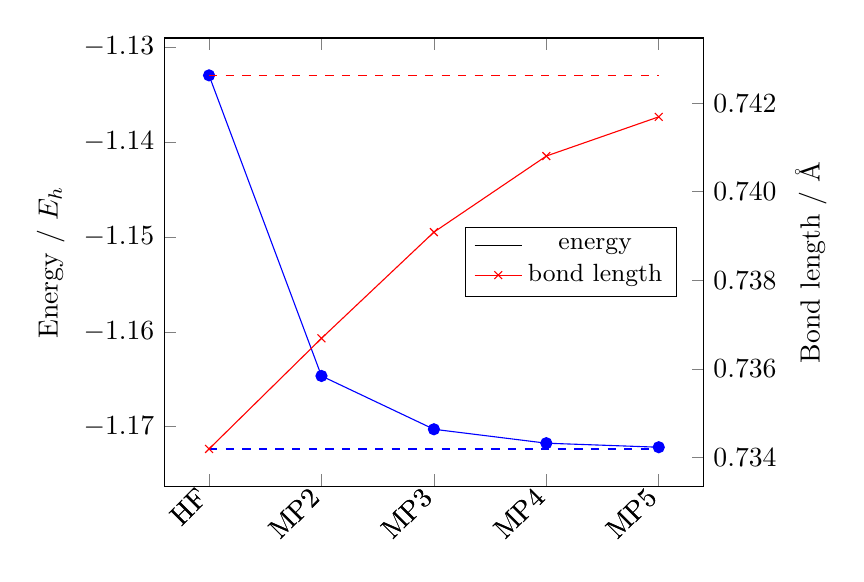
\begin{tikzpicture}
            \begin{axis}[
                axis y line*=left,
                ylabel={Energy / \(E_h\)},
                symbolic x coords={HF,MP2,MP3,MP4,MP5},
                xtick={HF,MP2,MP3,MP4,MP5},
                x tick label style={rotate=45,anchor=east},
            ]
                \addplot[blue,mark=*] coordinates {
                    (HF,-1.1329897) (MP2,-1.1646497) (MP3,-1.1702639) (MP4,-1.1717301) (MP5,-1.1721553)
                };\label{plot_one}
                \addplot[blue,dashed] coordinates {
                    (HF,-1.1723367) (MP5,-1.1723367)
                };
            \end{axis}
            \begin{axis}[
                axis y line*=right,
                ylabel={Bond length / \AA},
                y tick label style={
                    /pgf/number format/.cd,
                        fixed,
                        fixed zerofill,
                        precision=3,
                    /tikz/.cd
                },
                symbolic x coords={HF,MP2,MP3,MP4,MP5},
                xtick=data,
                x tick label style={rotate=45,anchor=east},
                legend style={at={(0.95,0.5)},
                anchor=east},
            ]   
                \addlegendimage{/pgfplots/refstyle=plot_one}\addlegendentry{\small energy}
                \addplot[red,mark=x] coordinates {
                    (HF,0.734196) (MP2,0.736692) (MP3,0.739088) (MP4,0.740805) (MP5,0.741690)
                };
                \addplot[red,dashed] coordinates {
                    (HF,0.742626) (MP5,0.742626)
                };
                \addlegendentry{\small bond length}
            \end{axis}
        \end{tikzpicture}
        \caption{The equilibrium geometry and bond length calculated using various methods with cc-pVTZ basis set. The full-CI result is included as the dashed line. Note that CCSD is equivalent to full-CI in two-electron systems.}
    \end{figure}

    \newpage
    \section{Self Consistent Field Gradient Theory (Non-examinable)}
    We are going to derive a formula for the gradient of the SCF energy, at a point \(\vb{X}\) on the SCF potential energy surface. Therefore we wish to calculate
    \begin{equation}
        \lim_{\delta\vb{X}\to 0}\frac{E(\vb{X}+\delta\vb{X})-E(\vb{X})}{\delta\vb{X}}=\dv{E}{\vb{X}}\,.
    \end{equation}
    At \(\vb{X}+\delta\vb{X}\), the orbitals \(\phi_i\) will have changed through their basis functions \(\eta_\alpha\) and through their molecular orbital coefficients \(c_{\alpha i}\).

    The change in the basis functions is easily evaluated. Consider a basis function \(\eta_\alpha\) which is an s-Gaussian \(\exp(-\alpha(\vb{x}-\vb{X})^2)\). Differentiating it with respect to centre \(\vb{X}\), we obtain
    \begin{equation}
        \dv{\eta_\alpha}{\vb{X}}=-2\alpha(\vb{X}-\vb{x})\exp(-\alpha(\vb{x}-\vb{X})^2)\,.
    \end{equation}
    This is a p-Gaussian. We denote it as \(\eta_\alpha^{\vb{X}}\).

    It is simplest to proceed using Lagrange multipliers. We wish to differentiate the energy maintaining orbital orthogonality. We therefore consider the function \(G(\vb{c},\vb{X})\), where
    \begin{equation}
        G(\vb{c},\vb{X})=E(\vb{c},\vb{X})-\sum_{i,j}\epsilon_{ij}(S_{ij}-\delta_{ij})\,.
    \end{equation}
    Here \(E(\vb{c},\vb{X})\) is the SCF energy expression in terms of molecular orbital integrals, \(S_{ij}\) is the overlap integral \(\braket{\phi_i}{\phi_j}\), and \(\epsilon_{ij}\) are the Lagrange multipliers. We know that
    \begin{equation}\label{Lagrange_coefficients_stationary}
        \pdv{G}{\vb{c}}=0
    \end{equation}
    because this is the SCF condition. Indeed it can be easily shown that (\ref{Lagrange_coefficients_stationary}) is equivalent to (\ref{HF_SCF_secular}) if we use orbitals which diagonalise the Lagrangian matrix, and in this case \(\epsilon_{ii}=\epsilon_i\), the orbital energies. In this case
    \begin{equation}
        G(\vb{c},\vb{X})=E(\vb{c},\vb{X})-\sum_i\epsilon_i(S_{ii}-1)\,.
    \end{equation}
    The expression for the gradient of the energy is
    \begin{equation}
        \dv{G}{\vb{X}}=\pdv{G}{\vb{c}}\dv{\vb{c}}{\vb{X}}+\pdv{G}{\vb{X}}\,.
    \end{equation}
    The first term is zero by (\ref{Lagrange_coefficients_stationary}), and thus the expression for the energy gradient is
    \begin{equation}
        \dv{G}{\vb{X}}=\pdv{G}{\vb{X}}=\pdv{E}{\vb{X}}-\sum_i\epsilon_i\pdv{S_{ii}}{\vb{X}}\,.
    \end{equation}
    Using the superscript notation introduced above to denote differentiation with respect to basis functions only, we have the expression for the energy gradient
    \begin{equation}
        \dv{E}{\vb{X}}=E^{\vb{X}}-\sum_i\epsilon_i S_{ii}^{\vb{X}}\,,
    \end{equation}
    where, for example,
    \begin{align}
        S_{ii}^{\vb{X}}&=2\braket{\phi_i^{\vb{X}}}{\phi_i}=\sum_{\alpha,\beta}c_{\alpha i}c_{\beta i}S_{\alpha\beta}^{\vb{X}}\notag\\
        &=\sum_{\alpha,\beta}c_{\alpha i}c_{\beta i}[\braket{\eta_\alpha^{\vb{X}}}{\eta_\beta}+\braket{\eta_{\alpha}}{\eta_{\beta}^{\vb{X}}}]\,.
    \end{align}
    We can now write the expression for the gradient of the closed-shell SCF energy in terms of differentiated basis function integrals and some density matrices
    \begin{equation}\label{HF_SCF_energy_gradient}
        \dv{E}{\vb{X}}=2\sum_{\alpha,\beta}D_{\alpha\beta}h_{\alpha\beta}^{\vb{X}}+\sum_{\alpha,\beta,\gamma,\delta}D_{\alpha\beta}D_{\gamma\delta}[2\bracket{\alpha\beta}{\gamma\delta}^{\vb{X}}-\bracket{\alpha\gamma}{\beta\delta}^{\vb{X}}]-2\sum_{\alpha\beta}E_{\alpha\beta}S_{\alpha\beta}^{\vb{X}}\,,
    \end{equation}
    where
    \begin{align}
        \bracket{\alpha\beta}{\gamma\delta}^{\vb{X}}&=\bracket{\alpha^{\vb{X}}\beta}{\gamma\delta}+\bracket{\alpha\beta^{\vb{X}}}{\gamma\delta}+\bracket{\alpha\beta}{\gamma^{\vb{X}}\delta}+\bracket{\alpha\beta}{\gamma\delta^{\vb{X}}}\,,\\
        h_{\alpha\beta}^{\vb{X}}&=\mel{\alpha^{\vb{X}}}{h}{\beta}+\mel{\alpha}{h}{\vb{\beta}^{\vb{X}}}+\mel{\alpha}{h^{\vb{X}}}{\beta}\,,\\
        D_{\alpha\beta}&=\sum_{i} c_{\alpha i}^* c_{\beta i}\,,\\
        E_{\alpha\beta}&=\sum_{i} \epsilon_i c_{\alpha i}^* c_{\beta i}\,.
    \end{align}

    Equation (\ref{HF_SCF_energy_gradient}) shows that a knowledge of the density matrices \(\mathsf{D}\), \(\mathsf{E}\) (available following the SCF calculation) and differentiated basis function integrals lead directly to the energy gradient; it is therefore a very easy computational procedure and an extremely important one for quantum chemistry, the Hartree--Fock geometry of a molecule can now be determined efficiently.
    
    \newpage
    \section{Multi-Configurational Methods}
    Not all systems are even moderately well described by a single Slater determinant, and these are known as \textit{multi-reference systems}, as there is more than one sensible reference Slater determinant. Such situations commonly arise when bond breakings or degeneracies are involved (e.g. for transition metals). In such cases, the single-determinant Hartree--Fock equations usually have multiple solutions close in energy to each other.

    The way to proceed in such systems is to do \textit{multi-configurational SCF} (MCSCF) theory where the wavefunction is expressed as a limited Slater determinant expansion, \(\Psi=\sum_I C_I\Phi_I\), and we find
    \begin{equation}
        \min_{\{c_{\mu_i}\},\{C_I\}}\expval{\hat{H}}{\Psi}\,.
    \end{equation}
    This method can be considered a combination between configuration interaction (where the molecular orbitals are not varied but the expansion of the wavefunction is) and Hartree--Fock (where there is only one determinant, but the molecular orbitals are varied).
    
    The determinants \(\Phi_I\) are made from the set of orbitals, and can be chosen by hand or as a \textit{complete active space} CAS(\(e\),\(o\)), where \(e\) is the number of active electrons and \(o\) is the number of active orbitals. Such calculation is known as \textit{complete active space self-consistent field} (CASSCF).

    \begin{figure}[ht!]
        \centering
        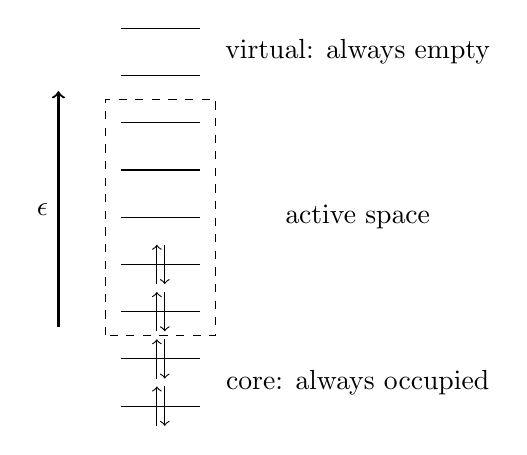
\begin{tikzpicture}
            \foreach \x in {0,...,8}{
                \draw (0,0.6*\x)--(1,0.6*\x);
            }
            \draw[->,thick] (-0.8,1)--node[left]{\(\epsilon\)}(-0.8,4);
            \foreach \x in {0,...,3}{
                \draw[->] (0.45,-0.25+0.6*\x)--(0.45,0.25+0.6*\x);
                \draw[<-] (0.55,-0.25+0.6*\x)--(0.55,0.25+0.6*\x);
            }
            \draw[dashed] (-0.2,0.9) rectangle (1.2,3.9);
            \node at (3,0.3) {core: always occupied};
            \node at (3,2.4) {active space};
            \node at (3,4.5) {virtual: always empty};
        \end{tikzpicture}
        \caption{In this example, we would like to consider all possible Slater determinants in CAS(4e,5o). It picks up the non-dynamic correlation.}
    \end{figure}
    \subsection{Correlation}
    We need to extend MCSCF to include dynamic correlations. Most single-reference methods have an extension to a multi-reference version, where MCSCF wavefunctions are often used as reference states, but usually with some drawbacks.

    \textit{Complete active space configuration interaction} (CASCI) or \textit{multi-reference configuration interaction} (MRCI) makes a space of single and double (and sometimes triple) excitations of all the determinants in the reference wavefunction, and diagonalises the Hamiltonian in this space. As for single-reference CI, it is not size-consistent and is quite computationally expensive.

    \textit{Complete active space perturbation theory} (CASPT2) extends M\o ller--Plesset perturbation theory to a CAS reference function. Among such calculations it is relatively widely used, but requires a lot of skill to set up calculations and suffers from \textit{intruder state problems} (if there exists \(E_I\) for an excited state \(\Phi_I\) that has similar energy to one in the active space, the denominator in the perturbation energy will be close to zero, and the energy will blow up).

    \textit{Multi-reference coupled cluster} (MRCC) method suffers from a difficulty of defining what excitations to include in \(\hat{T}\) and are generally quite computationally expensive as well as losing the size-consistency inherent in the CC ansatz.
    
    \subsection{Valence Bond Methods}
    \textit{Valence bond} (VB) methods are an attempt to form the wavefunction explicitly in terms of bonds. A simple form of the hydrogen molecule wavefunction is
    \begin{equation}
        \Psi_{\text{VB}}=\frac{1}{\sqrt{2(1+S^2)}}(\phi_1(1)\phi_2(2)+\phi_2(1)\phi_1(2))\frac{1}{\sqrt{2}}(\alpha(1)\beta(2)-\beta(1)\alpha(2))\,,
    \end{equation}
    where \(\phi_1\) and \(\phi_2\) are non-orthogonal atomic orbitals centred on nucleus 1 and 2 respectively, so overlap \(S=\braket{\phi_1}{\phi_2}\) is nonzero.

    A more general form of this allows variational flexibility, forming non-orthogonal orbitals \(u\) and \(v\) expanded in a basis set
    \begin{equation}
        \Psi_{\text{GVB}}=\frac{1}{\sqrt{2(1+S^2)}}(u(1)v(2)+v(1)u(2))\frac{1}{\sqrt{2}}(\alpha(1)\beta(2)-\beta(1)\alpha(2))\,,
    \end{equation}
    with \(S=\braket{u}{v}\).

    The GVB has a simple form that dissociates H\(_2\) correctly, but generalisations to many more electrons quickly become complicated. These equations are also hard to solve, with multiple solutions.

    \subsection{Non-Orthogonal CI}
    The Hartree--Fock SCF equations also have multiple solutions, corresponding to stationary points and local minima on the potential energy surface. It is possible to retain the attractive features of HF theory (size-consistency and low computational cost), and include multi-reference character by enumerating the low-energy SCF solutions, \(\{\Phi_x\}\), and performing configuration interaction with them. Define
    \begin{align}
        H_{xy}&=\mel{\Phi_x}{\hat{H}}{\Phi_y}\,,\\
        S_{xy}&=\braket{\Phi_x}{\Phi_y}\,,
    \end{align}
    then we need to solve the secular equation
    \begin{equation}
        \sum_{y}H_{xy}C_y=E\sum_{y}S_{xy}C_y\,.
    \end{equation}
    The orbitals in state \(x\) are different and not orthogonal to those in state \(y\), so the Slater--Condon rules cannot be used. L\"{o}wdin's method of corresponding orbitals allows for a generalisation of the Slater--Condon rules, and the generalised eigenvalue problem (including \(S_{xy}\)) must be solved. The solutions are however variational and size-consistent where the requisite SCF states can be located.

    \newpage
    \part{Density Functional Theory}
    \section{Schr\"{o}dinger Equation}
    The basic equation of Quantum Mechanics is given by the Schr\"{o}dinger equation
    \begin{equation}
        \hat{H}\Psi=E\Psi\,,
    \end{equation}
    with the Hamiltonian
    \begin{equation}
        \hat{H}=\sum_i-\frac{1}{2}\laplacian_i +\sum_i v(\vb{r}_i)+\sum_{i>j}\frac{1}{\norm{\vb{r}_i-\vb{r}_j}}\,.
    \end{equation}
    The ground state energy \(E_0\) of the system is given by finding the ground state many electron wavefunction \(\Psi(\vb{r}_1,\vb{r}_2,\dots,\vb{r}_N)\). This can also be written as
    \begin{equation}
        E_0=\min_{\norm{\Psi}=1}\expval{\hat{H}}{\Psi}\,.
    \end{equation}
    For example the Hartree--Fock solution is by minimising the energy with the constraint that the wavefunction is given by a single Slater determinant
    \begin{equation}
        E_0=\min_{\Psi\in\{\Psi_{\text{SD}}\}}\expval{\hat{H}}{\Psi}\,.
    \end{equation}
    
    To go beyond the Hartree--Fock approximation, the wavefunction has to be improved; generally this is done by including other determinants. Methods such as M\o ller--Plesset theory and coupled cluster theory have become very widely used for standard chemical problems. For more complicated electronic structure problems multi-reference methods have also been widely used.

    However the expansion of the wavefunction is costly. Hartree--Fock scales like \(N^4\), MP2 like \(N^5\), CCSD like \(N^6\) and full-CI scales like \(\e^N\). For small molecules the computational requirements are modest, though the scaling of the methods means that they quickly become prohibitively expensive and even the great advances made in computing and development of algorithms still make the need for other computational methods.

    Converging full-CI to the basis set limit is the ultimate benchmark method, though in general unnecessarily expensive compared to basis-set-extrapolated coupled cluster calculations. Nevertheless CI calculations are still performed on multi-configurational systems, generally using a Complete Active Space (CAS). The largest conventional CI calculation to date has only been carried out on the (22e,22o) active space of pentacene, with some \(1.2\times 10^{11}\) Slater determinants of the appropriate symmetry, though much larger systems have been studied by approximating the solutions (see \cref{Chap:FCIQMC}). This still makes the prospect of solving the Schr\"{o}dinger equation for condensed phase chemical reactions look impossibly far in the future.

    \begin{quote}
        \textit{``The fundamental laws necessary for the mathematical treatment of a large part of physics and the whole of chemistry are thus completely known, and the difficulty lies only in the fact that application of these laws leads to equations that are too complex to be solved.''}

        \hfill Paul A. M. Dirac (1929)
    \end{quote}

    Computers have helped greatly but still the direct solution of the Schr\"{o}dinger equation is a big challenge and a current area of research as outlined in the first half of the course. The complexity is all in the wavefunction, (ignoring spin) and the probability of finding electron 1 at \(\vb{r}_1\), electron 2 at \(\vb{r}_2\) and so on is given by \(\abs{\Psi(\vb{r}_1,\vb{r}_2,\dots,\vb{r}_N)}^2\). The electrons are indistinguishable so the probability to find any electron at a given point \(\vb{r}\) is given by
    \begin{equation}
        \rho(\vb{r})=\int\prod_{i=1}^{N}\dd[3]{\vb{r}_i}\abs{\Psi(\vb{r}_1,\dots,\vb{r}_N)}^2\sum_{j=1}^{N}\delta(\vb{r}_j-\vb{r})\,.
    \end{equation}
    This probability is the \textit{electron density}, \(\rho(\vb{r})\). It is a physical observable and no matter how many electrons are in the system it is only a real function of three dimensions \(\rho:\mathbb{R}^3\to\mathbb{R}\).

    \newpage
    \section{Density Functional Theory}
    \textit{Density functional theory} (DFT) is an alternative to wavefunction-based theories and is grounded on the fact that the electron density, which is a physically measurable quantity, contains all the information required to determine the ground-state electronic energy of a system. More formally, this means that given a ground state electron density \(\rho(\vb{r})\), there is a unique value of the electronic energy, \(E\). This means that the energy is a \textit{functional} of the density, and is denoted
    \begin{equation}
        E[\rho(\vb{r})]\,.
    \end{equation}
    We use the properties of the density and of functionals to give a proof of this below.
    \subsection{Functionals and Functional Derivatives}
    \begin{defn}
        A \textit{functional} is a special type of function that maps functions to values. Let \(X\) be a space of functions, then
        \begin{align}
            F:X&\to\mathbb{R}\notag\\
            y&\mapsto F[y]
        \end{align}
        is a functional.
    \end{defn}

    The analogue to differentiation of a function is the \textit{functional derivative}. It can be thought of as the change in the value of the functional when its function argument is changed by an infinitesimal amount.

    \begin{defn}
        Let \(F:V\to\mathbb{R}\) be a functional and \(\rho,\phi\in V\). The \textit{functional differential} of \(F\) at \(\rho\) in the direction of \(\phi\) is defined as the directional derivative
        \begin{align}
            \delta F[\rho,\phi]&=\lim_{\epsilon\to 0}\frac{F[\rho+\epsilon\phi]-F[\rho]}{\epsilon}\notag\\
            &=\left.\dv{}{\epsilon}\right|_{\epsilon=0} F[\rho+\epsilon\phi]
        \end{align}
    \end{defn}

    In most cases, the domain of the functional \(F\) is a space of differentiable functions \(\rho\) defined on some space \(\Omega\subset\mathbb{R}^n\) and \(F\) is of the form
    \begin{equation}
        F[\rho]=\int_{\Omega}\dd[n]{\vb{x}}L(\vb{x},\rho(\vb{x}),D\rho(\vb{x}))
    \end{equation}
    for some function \(L\), where \(D\rho\) denotes the derivative of \(\rho\). If this is the case, then we may define the \textit{functional derivative} of \(F\).
    \begin{defn}
        A functional of the form
        \begin{equation}
            F[\rho]=\int_{\Omega}\dd[n]{\vb{x}}L(\vb{x},\rho(\vb{x}),D\rho(\vb{x}))
        \end{equation}
        is \textit{differentiable} if there exists a function \(\delta F/\delta \rho\) such that
        \begin{equation}
            \delta F[\rho,\phi]=\int_{\Omega}\dd[n]{\vb{x}}\frac{\delta F}{\delta \rho}(\vb{x})\phi(\vb{x})\,.
        \end{equation}
        Then \(\delta F/\delta \rho\) is the \textit{functional derivative} of \(F\) at \(\rho\).
    \end{defn}
    If \(F\) is restricted to only certain functions \(\rho\) (for example, if there are some boundary conditions imposed) then \(\phi\) is restricted to functions such that \(\rho+\epsilon\phi\) continues to satisfy these conditions. Heuristically, \(\phi\) is the change in \(\rho\), so we formally have \(\phi=\delta \rho\).

    \begin{lem}
        Let
        \begin{equation}
            G[y]=\int_{\alpha}^{\beta}\dd{x}f(x,y,y')
        \end{equation}
        be a functional of \(y:\mathbb{R}\to\mathbb{R}\) smooth and restricted to some constant values at its boundary. Then the functional derivative of \(G\) is
        \begin{equation}
            \frac{\delta G}{\delta y}=\pdv{f}{y}-\dv{}{x}\left(\pdv{f}{y'}\right)\,.
        \end{equation}
    \end{lem}
    \begin{proof}
        For \(\norm{\delta y}\to 0\),
        \begin{align}
            \delta G&=\int_{\alpha}^{\beta}\dd{x}f(y+\delta y,y'+\delta y';x)-\int_{\alpha}^{\beta}\dd{x}f(y,y';x)\notag\\
            &=\int_{\alpha}^{\beta}\dd{x}\left[f(y,y';x)+\delta y\pdv{f}{y}+(\delta y)'\pdv{f}{y'}+\dots\right]-\int_{\alpha}^{\beta}\dd{x}f(y,y';x)\notag\\
            &=\int_{\alpha}^{\beta}\dd{x}\delta y\pdv{f}{y}+\left[\delta y\pdv{f}{y'}\right]_\alpha^\beta-\int_{\alpha}^{\beta}\dd{x}\delta y\dv{}{x}\left(\pdv{f}{y'}\right)+\dots
        \end{align}
        Therefore, when \(\delta y(\alpha)=\delta y(\beta)=0\),
        \begin{equation}
            \delta G=\int_{\alpha}^{\beta}\dd{x}\delta y\left[\pdv{f}{y}-\dv{}{x}\left(\pdv{f}{y'}\right)\right]\,.
        \end{equation}\qed
    \end{proof}
    \begin{rem}
        We may alternatively define the functional derivative of a function \(G\) as
        \begin{equation}
            \frac{\delta G}{\delta y(x)}\coloneqq\lim_{\epsilon\to 0}\frac{G[y(u)+\epsilon\delta(u-x)]-G[y(u)]}{\epsilon}\,,
        \end{equation}
        if this limit exists. Although this definition is a bit awkward and involves the delta function, it depends only on the functional \(G\) and its argument \(y\). It can be shown that this definition is consistent with the theorem above.
        \begin{align}
            \int_{\alpha}^{\beta}\dd{x}\delta y(x) \frac{\delta G}{\delta y(x)}&=\int_{\alpha}^{\beta}\dd{x}\delta y(x)\lim_{\epsilon\to 0}\frac{G[y+\epsilon\delta(x-y)]-G[y]}{\epsilon}\notag\\
            &=\int_{\alpha}^{\beta}\dd{x}\delta y(x)\lim_{\epsilon\to 0}\bigg[\int_{\alpha}^{\beta}\dd{u}f(u,y(u,\epsilon\delta(u-x)),y'(u)+\epsilon\delta'(u-x)) \notag\\
            &\quad -f(u,y(u),y'(u))\bigg]\frac{1}{\epsilon}\notag\\
            &=\int_{\alpha}^{\beta}\dd{x}\delta y(x)\lim_{\epsilon\to 0}\frac{1}{\epsilon}\left[\int_{\alpha}^{\beta}\dd{u}\pdv{f}{y}\epsilon\delta(u-x)+\pdv{f}{y'}\delta'(u-x)\right]\notag\\
            &=\int_{\alpha}^{\beta}\dd{x}\delta y(x)\left[\pdv{f}{y}-\dv{}{x}\left(\pdv{f}{y'}\right)\right]\,.
        \end{align}
    \end{rem}
    \begin{thm}[Euler--Lagrange equation]
        Let \(y(x)\) be a real, smooth function with fixed values at \(x=\alpha\) and \(x=\beta\). The functional
		\begin{equation}
			G[y]=\int_{\alpha}^{\beta}\dd{x}f(x,y,y')
		\end{equation}
		is stationary if and only if
		\begin{equation}
            \dv{}{x}\left(\pdv{f}{y'}\right)=\pdv{f}{y}\,.
        \end{equation}
    \end{thm}
    \begin{proof}
        Trivial from above lemma.\qed
    \end{proof}
    \begin{prop}
        The functional derivative of
        \begin{equation}
            G[y]=\int\dd[n]{x}v(x)y(x)\,,
        \end{equation}
        is given by
        \begin{equation}
            \frac{\delta G}{\delta y(x)}=v(x)\,.
        \end{equation}
    \end{prop}
    \begin{proof}
        \begin{equation}
            \frac{\delta G}{\delta y}=\pdv{vy}{y}=v\,.
        \end{equation}\qed
    \end{proof}
    \begin{prop}
        The functional
        \begin{equation}
            F[\rho]=\int\dd[3]{\vb{r}}f(\vb{r},\rho(\vb{r}),\grad\rho(\vb{r}))
        \end{equation}
        has a functional derivative
        \begin{equation}
            \frac{\delta F}{\delta \rho(\vb{r})}=\pdv{f}{\rho(\vb{r})}-\div\pdv{f}{\grad\rho(\vb{r})}\,.
        \end{equation}
    \end{prop}
    \begin{proof}
        For \(\phi(\vb{r})\) that vanishes on the boundary of the region of integration,
        \begin{align}
            \int\dd[3]{\vb{r}}\phi(\vb{r})\pdv{F}{\rho(\vb{r})}&=\left.\dv{}{\epsilon}\right|_{\epsilon=0}\int\dd[3]{\vb{r}}f(\vb{r},\rho+\epsilon\phi,\grad\rho+\epsilon\grad\phi)\notag\\
            &=\int\dd[3]{\vb{r}}\left(\pdv{f}{\rho}\phi+\pdv{f}{\grad\rho}\cdot\grad\phi\right)\notag\\
            &=\int\dd[3]{\vb{r}}\left[\pdv{f}{\rho}\phi+\div\left(\pdv{f}{\grad\rho}\phi\right)-\left(\div\pdv{f}{\grad\rho}\right)\phi\right]\notag\\
            &=\int\dd[3]{\vb{r}}\left[\pdv{f}{\rho}\phi-\left(\div\pdv{f}{\grad\rho}\right)\phi\right]\notag\\
            &=\int\dd[3]{\vb{r}}\left(\pdv{f}{\rho}-\div\pdv{f}{\grad\rho}\right)\phi\,,
        \end{align}
        where the second line is obtained using the total derivative, the third line is obtained by use of a product rule for divergence, and the fourth line is obtained using the divergence theorem and the condition that \(\phi =0\) on the boundary of the region of integration.\qed
    \end{proof}
    \subsection{The Density}
    We define \(\vb{r}_i\) to be the spatial coordinate, \(s_i\) to be the abstract spin coordinate and \(\vb{x}_i\coloneqq(\vb{r}_i, s_i)\).

    As a result of the Born--Oppenheimer approximation, the Coulomb potential arising from the nuclei is treated as a static external potential
    \begin{equation}
        V\ext(\vb{r})=v(\vb{r})\equiv -\sum_{\alpha}\frac{Z_{\alpha}}{\norm{\vb{r}-\vb{r}_{\alpha}}}\,.
    \end{equation}
    We use \(V\ext\) for a general potential and \(v\) for the nuclear-electron potential specifically. We define the remainder of the electronic Hamiltonian as
    \begin{equation}
        \hat{F}\coloneqq\hat{T}+\hat{V}\ee=-\frac{1}{2}\sum_i\laplacian_i+\sum_{i>j}\frac{1}{\norm{\vb{r}_i-\vb{r}_j}}
    \end{equation}
    such that
    \begin{equation}
        \hat{H}=\hat{F}+\hat{V}\ext\,,
    \end{equation}
    where
    \begin{equation}
        \hat{V}\ext=\sum_i V\ext(\vb{r}_i)\,.
    \end{equation}
    \(\hat{F}\) is the same for all \(N\)-electron systems, so the Hamiltonian, and hence the ground state \(\ket{\Psi_0}\) are completely determined by \(N\) and \(V\ext(\vb{r})\). The ground state \(\ket{\Psi_0}\) of this Hamiltonian gives rise to a ground state electronic density
    \begin{equation}
        \rho(\vb{r}_1)=N\int\dd{s_1}\prod_{i=2}^{N}\dd[4]{\vb{x}_i}\abs{\Psi}^2\,.
    \end{equation}
    Note that \(\d[4]{\vb{x}_i}\equiv\dd{s_i}\d[3]{\vb{r}_i}\) integrates over both the spin and spatial coordinate of electron \(i\). We clearly have
    \begin{equation}\label{total_electron_density}
        \int\dd[3]{\vb{r}}\rho(\vb{r})=N\,.
    \end{equation}
    Thus the ground-state \(\ket{\Psi_0}\) and density \(\rho_0(\vb{r})\) are both functionals of the number of electrons \(N\) and the external potential \(V\ext(\vb{r})\).

    \subsection{Hohenberg--Kohn Theorems}
    Density functional theory, introduced in 1964 by Hohenberg and Kohn, makes two remarkable statements.
    
    \begin{thm}[The first Hohenberg--Kohn theorem]
        The external potential \(V\ext(\vb{r})\) and hence the total energy are unique functionals of the electron density \(\rho(\vb{r})\) up to an additive constant.
    \end{thm}
    \begin{proof}
        Suppose there are two external potentials \(V_{1}(\vb{r})\) and \(V_{2}(\vb{r})\) both lead to the same \(\rho(\vb{r})\). There will be two Hamiltonians \(\hat{H}_1\) and \(\hat{H}_2\) with the same ground state density, but different wavefunctions \(\Psi_1\) and \(\Psi_2\). Now use the variational principle,
        \begin{align}
            E_1^0<\expval{\hat{H}_1}{\Psi_2}&=\expval{\hat{H}_2}{\Psi_2}+\expval{\hat{H}_2-\hat{H}_1}{\Psi_2}\notag\\
            &=E_2^0+\int\dd[3]{\vb{r}}\rho(\vb{r})[V_1(\vb{r})-V_2(\vb{r})]\,,
        \end{align}
        where \(E_0^1\) and \(E_2^0\) are the ground state energies for \(\hat{H}_1\) and \(\hat{H}_2\), respectively. The subscripts 1 and 2 may be interchanged to give a second inequality. These two inequalities may be added to give
        \begin{equation}
            E_1^0+E_2^0<E_2^0+E_1^0\,,
        \end{equation}
        which is a contradiction.\qed
    \end{proof}
    Thus, at least in principle, the ground-state density determines (within a constant) the external potential of the Schr\"{o}dinger equation of which it is a solution. The external potential and number of electrons
    \begin{equation}
        N=\int\dd[3]{\vb{r}}\rho(\vb{r})
    \end{equation}
    determine all the ground-state properties of the system since the Hamiltonian and ground state wavefunction are determined by them.

    So for all densities \(\rho(\vb{r})\) which are ground state densities for some external potential (such a density is known as \textit{\(v\)-representable}), the functional
    \begin{equation}
        F[\rho]=\expval{\hat{F}}{\Psi}=\expval{\hat{T}+\hat{V}\ee}{\Psi}=T[\rho]+V\ee[\rho]
    \end{equation}
    is unique and well-defined, since \(\rho(\vb{r})\) determines the external potential and \(N\) (and therefore \({\hat F}\)) and thence \(\ket{\Psi}\). Now a functional for an arbitrary external potential \(V\ext(\vb{r})\) unrelated to the \(\tilde{V}\ext(\vb{r})\) determined by \(\rho(\vb{r})\) can be defined:
    \begin{equation}
        E_V[\rho]=F[\rho]+\int\dd[3]{\vb{r}}V\ext(\vb{r})\rho(\vb{r})\,.
    \end{equation}

    \begin{thm}[The second Hohenberg--Kohn theorem]
        For an arbitrary external potential \(V\ext\) and \(v\)-representable densities \(\rho(\vb{r})\) of \(N\) electrons,
        \begin{equation}\label{DFT_energy}
            E_V[\rho]=F[\rho]+\int\dd[3]{\vb{r}}V\ext(\vb{r})\rho(\vb{r})\ge E_0\,,
        \end{equation}
        where \(E_0\) is the ground state energy for \(N\) electrons in the external potential \(V\ext(\vb{r})\), and this functional reaches its minimum if and only if \(\rho\) is the true ground state electron density in such external potential \(V\ext\).
    \end{thm}
    \begin{proof}
        By the first theorem, a given \(\rho(\vb{r})\) determines its own external potential \(\tilde{V}\ext(\vb{r})\) and ground state \(\ket{\tilde{\Psi}}\). If this state is used as a trial state for the Hamiltonian with external potential \(V\ext(\vb{r})\), we have
        \begin{equation}
            \expval{\hat{H}}{\tilde{\Psi}}=\expval{\hat{F}}{\tilde{\Psi}}+\expval{\hat{V}\ext}{\tilde{\Psi}}=F[\rho]+\int\dd[3]{\vb{r}}V\ext(\vb{r})\rho(\vb{r})=E_V[\rho]\ge E_0
        \end{equation}
        by the variational principle. For non-degenerate ground states, equality holds if \(\ket{\tilde{\Psi}}\) is the ground state for the potential \(V\ext(\vb{r})\).\qed
    \end{proof}

    Thus the problem of solving the Schr\"{o}dinger equation for non-degenerate ground-states can be recast into a variational problem of minimising the functional \(E_V[\rho]\) with respect to \(v\)-representable densities.

    \begin{itemize}[topsep=0pt]
        \item An aside: Bright--Wilson proof of the first Hohenberg--Kohn theorem.
        
        If one knew the exact electron density, \(\rho(\vb{r})\), then the cusps of \(\rho(\vb{r})\) would occur at the positions of the nuclei. Furthermore, a knowledge of \(\norm{\grad\rho(\vb{r})}\) at the nuclei would give their nuclear charges, as it may be shown that the nuclear cusp condition gives
    \begin{equation}
        \left.\pdv{}{r}\right|_{r=0} \bar{\rho}(r)=-2Z\bar{\rho}(0)\,,
    \end{equation}
    where \(\bar{\rho}(r)\) is the average of \(\rho(\vb{r})\) on a sphere of radius \(r\) around the nucleus. Thus the full Schr\"{o}dinger Hamiltonian is known because it is completely defined once the position and charge of the nuclei are given. Hence, in principle (through full-CI), the wavefunction and energy are known, and thus everything is known. In conclusion, a knowledge of the density was all that was necessary for a complete determination of all molecular properties.
    \end{itemize}

    \subsubsection{Levy Constrained Search}
    The original Hohenberg--Kohn proof is restricted to non-degenerate ground states and \(\rho\) being \(v\)-representable. However, this is not a problem if we consider another alternative proof given by Levy. We define a functional of the density \(\rho(\vb{r})\) for the operator \(\hat{F}\) defined above as
    \begin{equation}
        F[\rho]=\min_{\ket{\Psi}\mapsto \rho}\expval{\hat{F}}{\Psi}\,,
    \end{equation}
    i.e. the functional taking the minimum value of the expectation value with respect to all states \(\ket{\Psi}\) which give the density \(\rho\). For a system with external potential \(V\ext(\vb{r})\) and ground state \(\ket{\Psi_0}\) with energy \(E_0\), consider a state \(\ket{\Psi_{[\rho]}}\), an \(N\)-electron state which yields density \(\rho(\vb{r})\) and minimises \(F[\rho]\). Define \(E_V[\rho]\) as
    \begin{equation}
        E_V[\rho]=F[\rho]+\int\dd[3]{\vb{r}}\rho(\vb{r})V\ext(\vb{r})=\expval{\hat{F}+\hat{V}\ext}{\Psi_{[\rho]}}\,.
    \end{equation} 
    Since \(\hat{H}=\hat{F}+\hat{V}\ext\), by the variational principle we obtain
    \begin{equation}\label{Levy_vp}
        E_V[\rho]\ge E_0\,,
    \end{equation}
    with equality if and only if \(\ket{\Psi_{[\rho]}}=\ket{\Psi_0}\). This holds for all densities which can be obtained from an \(N\)-electron wavefunction (such a density is said to be \(N\)-representable --- this is a weaker condition than \(v\)-representable). From the definition of \(F[\rho]\) we must also have
    \begin{equation}
        F[\rho_0]\le\expval{\hat{F}}{\Psi_0}\,,
    \end{equation}
    since \(\ket{\Psi_0}\) must be one of the states which yield \(\rho_0(\vb{r})\). Adding \(\int\dd[3]{\vb{r}}\rho_0(\vb{r})V\ext(\vb{r})\) gives
    \begin{equation}
        E_V[\rho_0]\le E_0\,.
    \end{equation}
    Hence, combining with (\ref{Levy_vp}) we have
    \begin{equation}
        E_V[\rho]\ge E_V[\rho_0]=E_0
    \end{equation}
    as desired.

    Thus the ground-state density \(\rho_0(\vb{r})\) minimises the functional \(E_V[\rho]\) and the minimum value is the ground-state electronic energy. Note that the requirement for non-degeneracy of the ground-state has disappeared, and further that instead of considering only \(v\)-representable densities, we can now consider \(N\)-representable densities. The requirements of \(N\)-representability are much weaker and satisfied by any well-behaved density, subjected to only a few conditions like non-negativity and proper differentiability.

    This variational principle allows us to write down the condition that the energy (\ref{DFT_energy}) is stationary with respect to changes in the density, subjected to the constraint that (\ref{total_electron_density}) holds:
    \begin{equation}
        \delta E_V[\rho]-\mu\delta\left[\int\dd[3]{\vb{r}}\rho(\vb{r})-N\right]=0\,,
    \end{equation}
    for which the stationary condition is, in terms of the functional derivative,
    \begin{equation}
        \mu=V\ext(\vb{r})+\frac{\delta F[\rho]}{\delta\rho(\vb{r})}\,.
    \end{equation}

    The importance of this theorem is its practicality, namely that if we assume that we have a good functional representation, then we can minimise it to get best density and structure. It is also the place where the ground state restriction enters, because the second Hohenberg--Kohn theorem can only be proved for the ground state.

    \newpage
    \section{Pure Density Functional Theory}
    \subsection{Thomas--Fermi Theory}
    The simplest example of a density functional theory came long before the Hohenberg--Kohn theorem and came not long after the introduction of the Schr\"{o}dinger equation. Thomas and Fermi used the density as the basic variable, using a model system of the uniform electron gas to define functionals with explicit approximations for \(T[\rho]\) and \(V\ee[\rho]\). For the \(T\) they took the kinetic energy of the uniform electron gas (see later), and the classical (or Hartree) electron-electron repulsion term for \(V\ee\)
    \begin{equation}
        J[\rho]=\frac{1}{2}\int\dd[3]{\vb{r}}\dd[3]{\vb{r}'}\frac{\rho(\vb{r})\rho(\vb{r}')}{\norm{\vb{r}-\vb{r}'}}\,.
    \end{equation}
    This gives an energy expression
    \begin{equation}
        E^{\text{TF}}[\rho]=\underbrace{\frac{3}{10}(3\pi^2)^{2/3}\int\dd[3]{\vb{r}}\rho^{5/3}}_{T[\rho]}+\underbrace{\frac{1}{2}\int\dd[3]{\vb{r}}\dd[3]{\vb{r}'}\frac{\rho(\vb{r})\rho(\vb{r}')}{\norm{\vb{r}-\vb{r}'}}}_{V\ee[\rho]=J[\rho]}+\int\dd[3]{\vb{r}}V\ext(\vb{r})\rho(\vb{r})\,.
    \end{equation}
    Minimisation of the energy expression leads to the \textit{Thomas--Fermi equation}
    \begin{equation}
        \frac{5}{3}c_{\text{F}}\rho^{2/3}(\vb{r})+\int\dd[3]{\vb{r}'}\frac{\rho(\vb{r}')}{\norm{\vb{r}-\vb{r}'}}+V\ext(\vb{r})=\mu\,,
    \end{equation}
    where \(c_F=3(3\pi^2)^{2/3}/10\).

    This is a beautiful and simple theory along the lines of the exact density functional theory however with approximate functionals. There was much  interest in understanding this theory, especially in the solid state community, where it was thought to be a good basis for the description of metals. However for chemistry Thomas--Fermi theory suffers from a devastating issue --- \textit{Teller's non-binding theorem}. The energy of a molecular system as a function of the nuclear coordinates
    \begin{equation}
        E(\vb{R})=E^{\text{TF}}[\rho;\vb{R}]+\sum_{A>B}\frac{Z_AZ_B}{\norm{\vb{R}_A-\vb{R}_B}}
    \end{equation}
    decreases as \(\norm{\vb{R}_A-\vb{R}_B}\to\infty\). No molecule is bound with respect to dissociation to its constituent atoms --- meaning that Thomas--Fermi model is not applicable to any molecular system. This illustrates the difficulty of using approximate functionals and here the especial difficulty in approximating \(T\). For atoms and molecules near equilibrium the \textit{virial theorem} can show that \(\langle T\rangle=-E\). The kinetic energy is a massive term and any approximation to it has a very large error.

    \subsection{Kinetic Energy Functionals}
    Aside from the uniform electron gas kinetic energy
    \begin{equation}
        T^{\text{UEG}}[\rho]=\frac{3}{10}(3\pi^2)^{2/3}\int\dd[3]{\vb{r}}\rho^{5/3}(\vb{r})\,,
    \end{equation}
    which is exact when \(\rho\) is constant, it has proven challenging to derive functionals for kinetic energy. For a one-electron system, the wavefunction is simply the square root of its density, and from this von Weizs\"{a}cker gave the functional form
    \begin{equation}
        T^{\text{vW}}[\rho]=\frac{1}{8}\int\dd[3]{\vb{r}}\frac{\norm{\grad\rho}^2}{\rho}\,.
    \end{equation}
    The problem of finding an accurate kinetic energy functional for more than one electron is a subject of ongoing research in \textit{orbital-free density functional theory}, but little progress has been made over the years and effort has generally been focused on the Kohn--Sham formulation instead.

    \newpage
    \section{Kohn--Sham Theory}
    The major step forward for the implementation of density functional theory came with the introduction of the Kohn--Sham equations. The key idea here is to consider a fictitious system of non-interacting electrons which has the same density as the fully interacting system. The non-interacting wavefunction is a single determinant of \(N\) non-interacting electrons in \(N\) orbitals \(\phi_i\)
    \begin{equation}
        \Phi_{\text{KS}}=\antisymm\phi_1\phi_2\dots\phi_N\,.
    \end{equation}

    The key part here is that for this non-interacting system the kinetic energy is known exactly. The non-interacting kinetic energy (or Kohn--Sham kinetic energy) \(T\s\) can be expressed in terms of the Kohn--Sham orbitals
    \begin{equation}
        T\s[\{\phi_i\}]=\sum_{i}^{N}\expval{\hat{T}}{\phi_i}\,,
    \end{equation}
    and the density is given by
    \begin{equation}
        \rho(\vb{r})=\sum_{i}^{N}\abs{\phi_i(\vb{r})}^2\,.
    \end{equation}
    In this form \(T\s\) is not strictly a functional of \(\rho\), but instead of \(\{\phi_i\}\) and hence we denote it as \(T\s[\{\phi_i\}]\). For any \(\rho\), we can partition it into orbitals \(\{\phi_i\}\) in many ways. Since we wish to find the minimal \(E[\rho]\), we define
    \begin{equation}
        T\s[\rho]=\min_{\{\phi_i\}\mapsto\rho}T\s[\{\phi_i\}]\,.
    \end{equation}

    The Kohn--Sham orbitals \(\phi_i(\vb{r})\) are eigenfunctions of an effective one-electron Hamiltonian
    \begin{equation}
        \hat{h}\s\phi_i=\epsilon_i\phi_i\,,
    \end{equation}
    where
    \begin{equation}
        \hat{h}\s=-\frac{1}{2}\laplacian+V\s(\vb{r})\,,
    \end{equation}
    and \(V\s\) is an as-yet determined potential. Hence, the Kohn--Sham Hamiltonian is
    \begin{equation}
        \hat{H}_{\text{KS}}=\sum_{i=1}^{N}\hat{h}\s(\vb{r}_i)\,.
    \end{equation}
    \(\Phi_{\text{KS}}\) is an eigenfunction of \(\hat{H}_{\text{KS}}\) not \(\hat{H}\), but \(\Phi_{\text{KS}}\) yields the same electron density as the true ground state wavefunction of \(\hat{H}\).
    
    We can therefore rewrite the total energy as
    \begin{align}
        E[\rho]&=T[\rho]+V\ee[\rho]+V\ext[\rho]\notag\\
        &=T\s[\rho]+J[\rho]+V\ext[\rho]+[(T[\rho]-T\s[\rho])+(V\ee[\rho]-J[\rho])]\,.
    \end{align}
    The last term is the important exchange-correlation functional which contains all the complicated many-body quantum effects
    \begin{equation}
        E\xc[\rho]=(T[\rho]-T\s[\rho])+(V\ee[\rho]-J[\rho])\,.
    \end{equation}
    If we take the total energy expression
    \begin{equation}
        E[\rho]=T\s[\rho]+\int\dd[3]{\vb{r}}\rho(\vb{r})v(\vb{r})+J[\rho]+E\xc[\rho]
    \end{equation}
    and minimise with respect to orbitals we get the famous Kohn--Sham equations
    \begin{equation}
        \left(-\frac{1}{2}\laplacian+v(r)+v_{J}(\vb{r})+v\xc(\vb{r})\right)\phi_i=\epsilon_i\phi_i\,,
    \end{equation}
    where the Coulomb potential is
    \begin{equation}
        v_{J}(\vb{r})=\int\dd[3]{\vb{r}'}\frac{\rho(\vb{r}')}{\norm{\vb{r}-\vb{r}'}}
    \end{equation}
    and the exchange-correlation potential is given by the functional derivative
    \begin{equation}
        v\xc=\frac{\delta E\xc}{\delta\rho(\vb{r})}\,.
    \end{equation}
    If, for example, the exchange-correlation functional takes the form
    \begin{equation}
        E\xc[\rho]=\int\dd[3]{\vb{r}}f\xc(\rho,\grad\rho)\,,
    \end{equation}
    then the calculus of variations gives
    \begin{equation}
        v\xc(\vb{r})=\frac{\delta E\xc}{\delta\rho(\vb{r})}=\pdv{f\xc}{\rho}-\div\pdv{f\xc}{\grad\rho}\,.
    \end{equation}
    All the complexity is now in one term: the exchange-correlation potential.

    As you can see, the electron density is solved by Kohn--Sham equations, which in turn depends on the electron density. Thus, we again use the self-consistent field method to iteratively solve \(\rho\).

    \newpage
    \section{The Density and Exact Relations}
    \subsection{One and Two Particle (Reduced) Density Matrices}
    Since the true Hamiltonian is made up from at most two-particle operators, it is possible to express the energy in terms of at most two-particle quantities, rather than the full many-particle wavefunction \(\Psi\). We form these by integrating over the many coordinates of all but a few electrons, producing \textit{reduced density matrices}. The one particle (real space) reduced density matrix is formed from the wavefunction
    \begin{equation}
        \rho_1(\vb{r}_1',\vb{r}_1)=N\int\dd{s_1}\prod_{i=2}^{N}\dd[4]{\vb{x}_i}\Psi^*(\vb{r}_1',s_1,\vb{x}_2,\dots)\Psi(\vb{r}_1,s_1,\vb{x}_2,\dots)\,.
    \end{equation}
    The `diagonal' of this is its value for \(\vb{r}_1'=\vb{r}_1\),
    \begin{equation}
        \rho_1(\vb{r}_1,\vb{r}_1)=N\int\dd{s_1}\prod_{i=2}^{N}\dd[4]{\vb{x}_i}\abs{\Psi(\vb{x}_1,\vb{x}_2,\dots)}^2\,,
    \end{equation}
    which is the usual electron density
    \begin{equation}
        \rho(\vb{r})=\rho_1(\vb{r},\vb{r})\,.
    \end{equation}
    This is the real-space analogue of density matrix \(D_{\mu\nu}\), related by
    \begin{equation}
        \rho_1(\vb{r}',\vb{r})=\sum_{\mu,\nu}\eta_{\mu}^*(\vb{r}')D_{\mu\nu}\eta_{\nu}(\vb{r})\,.
    \end{equation}

    To calculate general expectation values we need the two-particle density matrix \(\Gamma_2(\vb{r}_1',\vb{r}_2',\vb{r}_1,\vb{r}_2)\). For our purposes, we only need its diagonal
    \begin{align}
        \rho_2(\vb{r}_1,\vb{r}_2)&=\Gamma_2(\vb{r}_1,\vb{r}_2,\vb{r}_1,\vb{r}_2)\notag\\
        &=\frac{N(N-1)}{2}\int\dd{s_1}\dd{s_2}\prod_{i=3}^{N}\dd[4]{\vb{x}_i}\abs{\Psi(\vb{x}_1,\vb{x}_2,\vb{x}_3,\dots)}^2\,.
    \end{align}
    The factor \(N(N-1)/2\) in front is the number of equivalent pairs.

    The energy, \(E\), given as the expectation value of the Hamiltonian can be expressed in terms of these matrices
    \begin{equation}
        E=-\frac{1}{2}\int\dd[3]{\vb{r}}\left.[\laplacian_{\vb{r}}\rho_1(\vb{r}',\vb{r})]\right|_{\vb{r}'=\vb{r}}+\int\dd[3]{\vb{r}}v(\vb{r})\rho(\vb{r})+\int\dd[3]{\vb{r}_1}\dd[3]{\vb{r}_2}\frac{\rho_2(\vb{r}_1,\vb{r}_2)}{\norm{\vb{r}_1-\vb{r}_2}}\,.
    \end{equation}
    In closed-shell restricted Hartree--Fock or Kohn--Sham theory the wavefunction is a single Slater determinant, and the one particle density matrix and the density are expressed in terms of spatial orbitals
    \begin{align}
        \rho_1(\vb{r}',\vb{r})&=2\sum_i\phi_i^*(\vb{r}')\phi_i(\vb{r})\,,\\
        \rho(\vb{r})&=2\sum_i\abs{\phi_i(\vb{r})}^2\,.
    \end{align}

    In Hartree--Fock theory, the exchange energy is
    \begin{align}
        K&=-\int\dd[3]{\vb{r}_1}\dd[3]{\vb{r}_2}\sum_{i,j}\frac{\phi_i^*(\vb{r}_1)\phi_i(\vb{r}_2)\phi_j^*(\vb{r}_2)\phi_j(\vb{r}_1)}{\norm{\vb{r}_1-\vb{r}_2}}\notag\\
        &=-\frac{1}{4}\int\dd[3]{\vb{r}_1}\dd[3]{\vb{r}_2}\frac{\abs{\rho_1(\vb{r}_1,\vb{r}_2)}^2}{\norm{\vb{r}_1-\vb{r}_2}}\,.
    \end{align}
    \subsection{Scaling Relations}
    Scaling relations have proven important in the development of some exact conditions for the exchange and correlation functionals. If we consider the normalisation of the density
    \begin{equation}
        \int\dd[3]{\vb{r}}\rho(\vb{r})=N
    \end{equation}
    and we introduce a change of variables \(\vb{r}=\lambda\vb{r'}\), then we have
    \begin{align}
        \int\dd[3]{\vb{r}'}\lambda^3\rho(\lambda\vb{r}')&=N\notag\\
        \Rightarrow\quad\int\dd[3]{\vb{r}}\lambda^3\rho(\lambda\vb{r})&=N\,.
    \end{align}
    We can define the \textit{scaled density}
    \begin{equation}
        \rho_{\lambda}(\vb{r})=\lambda^3\rho(\lambda\vb{r})
    \end{equation}
    such that
    \begin{equation}
        \int\dd[3]{\vb{r}}\rho_\lambda(\vb{r})=N\,.
    \end{equation}

    We now consider the coordinate scaling of the exact exchange energy used in the scaled orbitals \(\phi_{i\lambda}(\vb{r})=\lambda^{3/2}\phi_{i}(\lambda\vb{r})\). We begin by writing the total exchange in terms of a contribution from pairs of orbitals
    \begin{equation}
        E\x[\{\phi_{i\lambda}\}]=\sum_{i,j}E\x[\phi_{i\lambda},\phi_{j\lambda}]\,.
    \end{equation}
    The scaling of each orbital-pair component is determined from
    \begin{align}
        E\x[\phi_{i\lambda},\phi_{j\lambda}]&=\frac{1}{2}\int\dd[3]{\vb{r}_1}\dd[3]{\vb{r}_2}\frac{\phi_{i\lambda}^*(\vb{r}_1)\phi_{j\lambda}(\vb{r}_1)\phi_{i\lambda}(\vb{r}_2)\phi_{j\lambda}^*(\vb{r}_2)}{\norm{\vb{r}_1-\vb{r}_2}}\notag\\
        &=\frac{\lambda^6}{2}\int\dd[3]{\vb{r}_1}\dd[3]{\vb{r}_2}\frac{\phi_i^*(\lambda\vb{r}_1)\phi_j(\lambda\vb{r}_1)\phi_i(\lambda\vb{r}_2)\phi_j^*(\lambda\vb{r}_2)}{\norm{\vb{r}_1-\vb{r}_2}}\notag\\
        &=\frac{\lambda}{2}\int\lambda^3\dd[3]{\vb{r}_1}\lambda^3\dd[3]{\vb{r}_2}\frac{\phi_i^*(\lambda\vb{r}_1)\phi_j(\lambda\vb{r}_1)\phi_i(\lambda\vb{r}_2)\phi_j^*(\lambda\vb{r}_2)}{\norm{\lambda\vb{r}_1-\lambda\vb{r}_2}}\notag\\
        &=\frac{\lambda}{2}\int\dd[3]{\lambda\vb{r}_1}\dd[3]{\lambda\vb{r}_2}\frac{\phi_i^*(\lambda\vb{r}_1)\phi_j(\lambda\vb{r}_1)\phi_i(\lambda\vb{r}_2)\phi_j^*(\lambda\vb{r}_2)}{\norm{\lambda\vb{r}_1-\lambda\vb{r}_2}}\notag\\
        &=\lambda E\x[\phi_i,\phi_j]\,.
    \end{align}
    Now we can use the above scaling relation to find out more about possible forms of the exchange density functionals. If we examine a functional of the form
    \begin{equation}
        E\x^{\text{local}}[\rho]=c\int\dd[3]{\vb{r}}\rho^k(\vb{r})\,,
    \end{equation}
    where `local' means that the integrand does not depend on the density at two different positions simultaneously. Then
    \begin{align}
        E\x^{\text{local}}[\rho_{\lambda}]&=c\int\dd[3]{\vb{r}}\lambda^{3k}\rho^k(\lambda\vb{r})\notag\\
        &=c\lambda^{3k-3}\int\dd[3]{\lambda\vb{r}}\rho^k(\lambda\vb{r})\,.
    \end{align}
    To satisfy the scaling requirement, we need \(3k-3=1\), and therefore \(k=4/3\).
    \subsection{Adiabatic Connection}
    Langreth and Perdew defined a family of Hamiltonians interpolating between the fully interacting Hamiltonian and the Kohn--Sham Hamiltonian which retain the same ground-state density. They parameterised this with constant \(\lambda\) which scales the electron-electron repulsion term
    \begin{equation}
        \hat{H}_\lambda=\hat{T}+\lambda\hat{V}\ee+\hat{V}_{\lambda}\,,
    \end{equation}
    where \(\hat{V}_\lambda=\sum_i v_\lambda(\vb{r}_i)\) is the result of a one-electron local potential \(v_\lambda(\vb{r})\). For each \(\hat{H}_\lambda\) there is an energy-minimising wavefunction \(\Psi_\lambda\) satisfying
    \begin{equation}
        \hat{H}_\lambda\Psi_\lambda=E_\lambda\Psi_\lambda\,.
    \end{equation}
    At each \(\lambda\), the one-electron potential \(v_\lambda(\vb{r})\) is chosen such that the density is kept the same as the full interacting density:
    \begin{equation}
        \int\prod_{i=2}^{N}\dd[3]{\vb{r}_i}\abs{\Psi_\lambda(\vb{r},\vb{r}_2,\dots)}^2=\rho_\lambda(\vb{r})=\rho(\vb{r})
    \end{equation}
    for all \(\lambda\); in particular \(\rho_0=\rho_1=\rho\). At \(\lambda=1\) we have the full interacting Hamiltonian
    \begin{equation}
        \hat{H}_1=\hat{T}+\hat{V}\ee+\sum_{i}v(\vb{r}_i)\,,
    \end{equation}
    and at \(\lambda=0\) we have the Kohn--Sham system
    \begin{equation}
        \hat{H}_0=\hat{T}+\sum_i v\s(\vb{r}_i)\,,
    \end{equation}
    where \(v\s=v+v_{\text{J}}+v\xc\). At each value of \(\lambda\), the wavefunction \(\Psi_\lambda\) will be different, even though it corresponds to the same density \(\rho(\vb{r})\). Since \(\Psi_{\lambda}\) is the minimum-energy eigenfunction of \(\hat{H}_\lambda\), we can think of this as a search over the wavefunctions which give density \(\rho\)
    \begin{align}
        E_\lambda&=\min_{\Psi_\lambda\mapsto\rho}\expval{\hat{H}_\lambda}{\Psi_\lambda}\notag\\
        &=\min_{\Psi_\lambda\mapsto\rho}\left(\expval{\hat{T}+\lambda\hat{V}\ee}{\Psi_\lambda}+\expval{\hat{V}_\lambda}{\Psi_\lambda}\right)\,.
    \end{align}
    For a given \(\lambda\), since \(\hat{V}_\lambda=\sum_i v_\lambda(\vb{r}_i)\) contains only local one-electron operators, its expectation value is dependent only on the density, \(\rho(\vb{r})\), and does not vary with \(\Psi_{\lambda}\). \(\Psi_{\lambda}\) therefore minimises \(\expval{\hat{T}+\lambda\hat{V}\ee}{\Psi_\lambda}\).

    Consider the derivative of this expectation value
    \begin{align}
        \pdv{}{\lambda}\expval{\hat{T}+\lambda\hat{V}\ee}{\Psi_\lambda}&=\pdv{}{\lambda'}\expval{\hat{T}+\lambda\hat{V}\ee}{\Psi_{\lambda'}}+\pdv{}{\lambda'}\expval{\hat{T}+\lambda\hat{V}\ee}{\Psi_{\lambda}}\notag\\
        &=0+\expval{\hat{V}\ee}{\Psi_{\lambda}}\,,
    \end{align}
    where the first term is zero by the Hellmann-Feynman theorem as \(\Psi_\lambda\) is the minimising wavefunction. Now integrate between 0 and 1 gives
    \begin{align}
        \int_{0}^{1}\dd{\lambda}\expval{\hat{V}\ee}{\Psi_\lambda}&=\int_{0}^{1}\dd{\lambda}\pdv{}{\lambda}\expval{\hat{T}+\lambda\hat{V}\ee}{\Psi_\lambda}\notag\\
        &=\expval{\hat{T}+\hat{V}\ee}{\Psi_1}-\expval{\hat{T}}{\Psi_0}\notag\\
        &=T[\rho]+V\ee[\rho]-T\s[\rho]\,.
    \end{align}
    Now subtract the Coulomb energy from both sides
    \begin{equation}
        T[\rho]+V\ee[\rho]-T\s[\rho]-J[\rho]=\int_{0}^{1}\dd{\lambda}\expval{\hat{V}\ee}{\Psi_\lambda}-J[\rho]\,.
    \end{equation}
    Define
    \begin{equation}
        W_\lambda\coloneqq\expval{\hat{V}\ee}{\Psi_\lambda}-J[\rho]\,,
    \end{equation}
    then we get
    \begin{equation}
        E\xc[\rho]=\int_{0}^{1}\dd{\lambda}W_\lambda\,.
    \end{equation}

    Thus if we know \(W_\lambda[\rho]\), we can use it to create an exchange-correlation functional. In the \(\lambda=0\) limit, we have
    \begin{align}
        W_0&=\expval{\hat{V}\ee}{\Psi_0}-J[\rho]\notag\\
        &=J[\rho]-K[\rho]-J[\rho]\notag\\
        &=-K[\rho]\eqqcolon E\x[\rho]\,,
    \end{align}
    which is the Hartree--Fock exchange energy of density \(\rho\). For \(\lambda=1\),
    \begin{align}
        W_1&=\expval{\hat{V}\ee}{\Psi_1}-J[\rho]\notag\\
        &=V\ee[\rho]-J[\rho]\,,
    \end{align}
    where \(V\ee(\rho)\) contains all two-electron Coulomb, exchange and correlation contributions. To make headway we consider that, for the exact exchange-correlation functional, the energy is identical to the FCI energy, \(E_0[\rho]=E_1[\rho]\), so
    \begin{equation}
        E_{0}[\rho]=T\s[\rho]+J[\rho]+E\xc[\rho]=E_1[\rho]=T[\rho]+V\ee[\rho]\,.
    \end{equation}
    Rearranging this we have
    \begin{equation}
        W_1=V\ee[\rho]-J[\rho]=T\s[\rho]-T[\rho]+E\xc[\rho]\,,
    \end{equation}
    and so
    \begin{equation}
        W_1-E\xc[\rho]=T\s[\rho]-T[\rho]\eqqcolon -T\corr[\rho]\,,
    \end{equation}
    where \(T\corr[\rho]\) is the correction to the non-interacting kinetic energy due to correlation.

    This form of the exchange-correlation functional is instructive as \(W_\lambda\) can be evaluated for model systems and approximated.
    \subsection{Asymptotic Behaviour of the Density}
    An exact result which is of value for the electron density is that asymptotically
    \begin{equation}
        \rho\sim\exp(-2\sqrt{2I_{\text{min}}}r)\,,
    \end{equation}
    where \(I_{\text{min}}\) is the exact first ionisation potential. We shall now prove this.

    Consider a point \(\vb{r}_N\) which is a long way from the molecule. The exact wavefunction for this molecule, which has \(N\) electrons may be written in this situation as
    \begin{equation}
        \Psi_N=\Psi_{N-1}\phi_N(\vb{r}_N)\,,
    \end{equation}
    since there is no chance of having two electrons at such a large distance. \(\Psi_{N-1}\) is the wavefunction of the cation. We may write the \(N\) electron Hamiltonian as \(\hat{H}_N=\hat{H}_{N-1}+\hat{h}_N\), with \(\hat{h}_N\) being the one electron Hamiltonian for the last electron.
    \begin{equation}
        \hat{H}_N=\underbrace{-\sum_{i=1}^{N-1}\frac{1}{2}\laplacian_i+\sum_I\sum_{i=1}^{N-1}\frac{-Z_I}{r_{iI}}+\sum_{i<j}^{N-1}\frac{1}{r_{ij}}}_{\hat{H}_{N-1}}\;\underbrace{-\frac{1}{2}\laplacian_N+\sum_I\frac{-Z_I}{r_{NI}}+\sum_{i=1}^{N-1}\frac{1}{r_{iN}}}_{\hat{h}_{N}}\,.
    \end{equation}
    An application of \(\hat{H}_N\) to \(\Psi_N\) yields
    \begin{align}
        \hat{H}_N\Psi_{N-1}\phi_N&=(\hat{H}_{N-1}\Psi_{N-1})\phi_N+\Psi_{N-1}\hat{h}_N\phi_N\\
        E_N\Psi_{N-1}\phi_N&=(E_{N-1}\Psi_{N-1})\phi_N+\Psi_{N-1}\hat{h}_N\phi_N\\
        E_N\phi_N&=E_{N-1}\phi_N+\hat{h}_N\phi_N\,,
    \end{align}
    so
    \begin{equation}
        (E_N-E_{N-1})\phi_N=\hat{h}_N\phi_N\,,
    \end{equation}
    or
    \begin{equation}
        -\frac{1}{2}\laplacian_N\phi_N-\frac{1}{r_N}\phi_N=-I_{\text{min}}\phi_N\,.
    \end{equation}
    At a large distance the behaviour of \(\phi_N\) is exponential, i.e. \(\phi_N\sim\exp(-\alpha r)\). Substitution yields \(\alpha^2=2I_{\text{min}}\). The asymptotic form of the density will be given by \(\phi_N(\vb{r}_N)^2\) and the result is obtained.

    \newpage
    \section{Approximate Exchange-Correlation Functionals}
    \subsection{Local Density Approximation}
    There is no straightforward way in which the exchange-correlation functional \(E\xc[\rho]\) can be systematically improved, unlike \textit{ab initio} quantum chemistry. In \textit{ab initio} quantum chemistry SCF can be systematically improved in principle to unlimited accuracy through configuration interaction or perturbation theory. One way forward in DFT is to start from a model for which there is an exact solution --- the uniform electron gas.

    It is defined as a large number \(N\) of electrons in a cube of volume \(V=l^3\), throughout which there is uniformly spread out a positive charge sufficient to make the system neutral. The uniform electron gas corresponds to the limit \(N\to\infty\), \(V\to\infty\), with density \(\rho=N/V\) remaining finite.

    We will now briefly indicate how the expressions for \(T\s[\rho]\) and \(E\x[\rho]\) are derived. The Kohn--Sham equations for the uniform electron gas are satisfied by plane wavefunctions
    \begin{equation}
        \phi_{\vb{k}}=\frac{1}{\sqrt{V}}\e^{\ii\vb{k}\cdot\vb{r}}
    \end{equation}
    where periodic boundary conditions require
    \begin{equation}
        \vb{k}=\frac{2\pi}{l}\vb{n}\,,\;\vb{n}\in\mathbb{Z}^3\,.
    \end{equation}
    The one particle density matrix is given by
    \begin{equation}
        \rho_1(\vb{r}_1,\vb{r}_2)=\frac{2}{V}\sum_{\vb{k}\text{ occupied}}\e^{-\ii\vb{k}\cdot(\vb{r}_1-\vb{r}_2)}\,,
    \end{equation}
    which, on replacing the sum by an integral with \(\dd[3]{\vb{n}}=(V/8\pi^3)\dd[3]{\vb{k}}\) yields
    \begin{align}
        \rho_1(\vb{r}_1,\vb{r}_2)&=\frac{1}{4\pi^3}\int\dd[3]{\vb{k}}\e^{-\ii\vb{k}\cdot(\vb{r}_1-\vb{r}_2)}\notag\\
        &=\frac{1}{4\pi^3}\int_{0}^{k_{\text{F}}}\dd{k}k^2\int\dd{\theta}\dd{\phi}\sin\theta \e^{-\ii\vb{k}\cdot\vb{r}_{12}}\,.
    \end{align}
    The \textit{Fermi level} \(k_F\) is defined by evaluating the density \(\rho(\vb{r})=\rho_1(\vb{r},\vb{r})\)
    \begin{equation}
        \rho(\vb{r})=\frac{k_{\text{F}}^3}{3\pi^2}\quad\Rightarrow\quad k_F=[3\pi^2\rho(\vb{r})]^{1/3}\,.
    \end{equation}
    The kinetic energy
    \begin{equation}
        T\s=\int\dd[3]{\vb{r}}\left[-\frac{1}{2}\laplacian_{\vb{r}}\rho_1(\vb{r}',\vb{r})\right]_{\vb{r}'=\vb{r}}
    \end{equation}
    is easily obtained. It is
    \begin{align}
        T\s[\rho]&=\frac{1}{8\pi^2}\int\dd[3]{\vb{r}}\int_{0}^{k_{\text{F}}}\dd{k}4\pi k^4\notag\\
        &=\frac{1}{10\pi^2}\int\dd[3]{\vb{r}}k_F^{5}\notag\\
        &=\frac{3}{10}(3\pi^2)^{2/3}\int\dd[3]{\vb{r}}\rho^{5/3}(\vb{r})\,.
    \end{align}

    To evaluate \(\rho_{1}(\vb{r}_1,\vb{r}_2)\) generally we introduce the coordinates
    \begin{equation}
        \vb{r}=\frac{\vb{r}_1+\vb{r}_2}{2}\,,\;\vb{s}=\vb{r}_1-\vb{r}_2
    \end{equation}
    and choose \(\vb{s}\) to lie on the \(k_z\) axis. The integral may then be evaluated to give the exact first order spinless density matrix
    \begin{equation}
        \rho_1(\vb{r}_1,\vb{r}_2)=3\rho(\vb{r})\frac{\sin t-t\cos t}{t^3}\,,
    \end{equation}
    where \(t\coloneqq k_{\text{F}}(\vb{r})\norm{\vb{s}}\). The complete result is
    \begin{align}
        T\s[\rho]=C_{\text{F}}\int\dd[3]{\vb{r}}\rho^{5/3}(\vb{r})\\
        E\x^{\text{LDA}}[\rho]=-C\x\int\dd[3]{\vb{r}}\rho^{4/3}(\vb{r})\,,
    \end{align}
    where we defined the constants
    \begin{align}
        C_{\text{F}}&=\frac{3}{10}(3\pi^2)^{2/3}\approx 2.8712\\
        C\x&=\frac{3}{4}\left(\frac{3}{\pi}\right)^{1/3}\approx 0.7386\,.
    \end{align}
    To derive the result for \(E\x^{\text{LDA}}\), we have used the result
    \begin{equation}
        \int_{0}^{\infty}\dd{t}(\sin t-t\cos t)^2 t^{-5}=\frac{1}{4}\,.
    \end{equation}
    The exchange energy is called the \textit{Dirac exchange energy} or sometimes \textit{Slater exchange energy}.

    It is usual to introduce the exchange energy per particle \(\epsilon\x\) as a function of \(r_s\), the radius of a sphere whose volume is the effective volume of an electron,
    \begin{equation}
        \frac{4}{3}\pi r_s^3=\frac{1}{\rho}\,.
    \end{equation}
    The results are
    \begin{equation}
        E\x^{\text{LDA}}[\rho]=\int\dd[3]{\vb{r}}\rho(\vb{r})\epsilon\x(r_s)\,,
    \end{equation}
    where
    \begin{equation}
        \epsilon\x^{\text{LDA}}=-\frac{0.4582}{r_s}\,.
    \end{equation}

    In the case when the alpha spin density is not equal to the beta spin density, the kinetic and exchange energies are
    \begin{align}
        T\s[\rho_\alpha,\rho_\beta]&=2^{2/3}C_{\text{F}}\int\dd[3]{\vb{r}}[\rho_\alpha^{5/3}+\rho_\beta^{5/3}]\,,\\
        E\x^{\text{LSDA}}[\rho_\alpha,\rho_\beta]&=-2^{1/3}C\x\int\dd[3]{\vb{r}}[\rho_\alpha^{4/3}+\rho_\beta^{4/3}]\,,
    \end{align}
    as may be verified by putting \(\rho_\alpha=\rho_\beta=\rho/2\) for the closed-shell case.

    The ground state total energy of the uniform electron gas is
    \begin{equation}\label{UEG_energy}
        E[\rho]=T\s[\rho]+\int\dd[3]{\vb{r}}\rho(\vb{r})V\ext(\vb{r})+J[\rho]+E\xc[\rho]+E_b\,,
    \end{equation}
    where \(E_b\) being the electrostatic energy of the positive background, which is equal to the Coulomb energy because the magnitude of the positive charge density \(n(\vb{r})\) is equal to \(\rho(\vb{r})\). Because the external potential is defined by
    \begin{equation}
        V\ext(\vb{r})=-\int\dd[3]{\vb{r}'}\frac{n(\vb{r}')}{\norm{\vb{r}-\vb{r}'}}\,,
    \end{equation}
    it follows that the second, third and fifth terms of (\ref{UEG_energy}) add to zero, and therefore
    \begin{align}
        E[\rho]&=T\s[\rho]+E\xc[\rho]\notag\\
        &=T\s[\rho]+E\x[\rho]+E\corr[\rho]\,, \label{UEG_energy_simp}
    \end{align}
    where we have now split up the exchange-correlation term into an exchange term plus a correlation term.

    For the correlation functional of the electron gas, reliance is placed on the numerical simulations of the uniform electron gas by Ceperley and Alder using the quantum Monte-Carlo method for several different values of \(r\s\). (They studied \(r\s=1,2,5,10,20,50,100\) for \(\zeta=0\) and \(1\)). The correlation energy was obtained by subtracting the kinetic and exchange energies from (\ref{UEG_energy_simp}). Also using analytic information for the high and the low density limit, Vosko, Wilk and Nusair gave the first accepted form for the correlation electron density per electron \(\epsilon\corr(r\s)\), which is defined such that
    \begin{equation}
        E\corr[\rho]=\int\dd[3]{\vb{r}}\rho(\vb{r})\epsilon\corr(r\s(\rho(\vb{r})))\,,
    \end{equation}
    which covers both the spin polarised and spin compensated cases.
    \begin{align}
        \epsilon\corr^{\text{LDA}}(r\s)&=\frac{A}{2}\left(\ln\frac{x^2}{X(x)}+\frac{2b}{Q}\tan^{-1}\frac{Q}{2x+b}\right.\notag\\
        &\quad \left.-\frac{bx_0}{X(x_0)}\left[\ln\frac{(x-x_0)^2}{X(x)}+\frac{2(b+2x_0)}{Q}\tan^{-1}\frac{Q}{2x+b}\right]\right)\,,
    \end{align}
    where \(x=r\s^{1/2}\), \(X(x)=x^2+bx+c\), \(Q=(4c-b^2)^{1/2}\), and \(A=0.0621814\), \(x_0=-0.409286\), \(b=13.0720\), \(c=42.7198\). It was later updated by Perdew and Wang to give the PW91 local correlation functional.

    This completes the description of the uniform electron gas and its functionals. The application of these functionals in chemistry is often referred to as the \textit{local density approximation} (LDA) or the \textit{local spin density approximation} (LSDA). For molecular chemistry the errors from LDA energies are often too large to be useful. The LDA also does not bind anions as \(\epsilon\x(\vb{r})\) decays too rapidly. Typical errors in \(E\x\) is usually \(5\%\) for being not negative enough, and \(E\corr\) are usually too negative by \(100\%\). The mean absolute error in atomisation energies is around \(180\unit{kJ}\unit{mol}^{-1}\).

    The main step forward for the introduction of DFT into chemistry was the introduction of the density gradient \(\grad\rho\).

    \subsection{Generalised Gradient Approximation}
    Let's first introduce the dimensionless reduced gradient density
    \begin{equation}
        x=\frac{\norm{\grad\rho}}{\rho^{4/3}}\,,
    \end{equation}
    and a related additional factor
    \begin{equation}
        s=\frac{x}{2(3\pi^2)^{1/3}}\,.
    \end{equation}
    It can be shown from the gradient expansion that for a slightly inhomogeneous electron gas with a slowly varying density, the exchange energy behaves like
    \begin{align}
        E\x^{\text{GEA2}}&=-\int\dd[3]{\vb{r}} c_{\text{D}}\rho^{4/3}+\frac{7}{432\pi(3\pi^2)^{1/3}}\frac{\norm{\grad\rho}^2}{\rho^{4/3}}\notag\\
        &\eqqcolon-\int\dd[3]{\vb{r}}c_{\text{D}}\rho^{4/3}+c_{x^2}\rho^{4/3}x^2\,,
    \end{align}
    where the Dirac exchange constant \(c_{\text{D}}=\frac{3}{4}(\frac{3}{\pi})^{1/3}\) and \(c_{x^2}=7/432(3\pi^2)^{1/3}\). This idea stems from the solid state however it did not take off in chemistry until the introduction of the \textit{generalised gradient approximation} (GGA) as the density in molecules is a long way from slowly varying. In fact in molecular tails where the density has an exponential decay then the reduced gradient diverges. This causes big problems for the direct use of the gradient expansion as can be clearly seen for the use of the fourth order correction where the energy diverges for any atom.

    Note that although GGA functionals make use of \(\grad\rho\) (via \(x\) or \(s\)), they are still local. The functionals don't require \(\rho\) at two different \(\vb{r}\) simultaneously. Using the gradient alleviates some of this locality.

    \begin{itemize}[topsep=0pt]
        \item Becke86
        \begin{equation}
            E\x^{\text{B86}}=E\x^{\text{LDA}}-\sum_{\sigma}\int\dd[3]{\vb{r}}\rho_\sigma^{4/3}\left(\frac{\beta\gamma x_\sigma^2}{1+\gamma x_\sigma^2}\right)\,.
        \end{equation}
        A simple form makes sure that the energy does not diverge as \(x\to\infty\). This is fitted to atomic exchange energies with \(\beta=0.0036\) and \(\gamma=0.004\).
        \item Becke88
        \begin{equation}
            E\x^{\text{B88}}=E\x^{\text{LDA}}-\sum_{\sigma}\int\dd[3]{\vb{r}}\rho_\sigma^{4/3}\left(\frac{\beta x_\sigma^2}{1+6\beta x_\sigma\sinh^{-1}(x_\sigma)}\right)\,.
        \end{equation}
        This is one of the most widely used exchange functionals in the literature. Its form was designed to give the correct asymptotic behaviour of the exchange energy density. However, its success is viewed more likely to be due to the procedure used to determine the constant \(\beta=0.0042\), a least squares fit to the Hartree--Fock exchange energies of the rare gas atoms (He-Kr).
        \item PBE
        \begin{equation}
            E\x^{\text{PBE}}=E\x^{\text{LDA}}-c_{\text{D}}\sum_\sigma \int\dd[3]{\vb{r}}\rho_\sigma^{4/3}\left(\kappa-\frac{\kappa}{1+\frac{\mu s_\sigma^2}{\kappa}}\right)\,,
        \end{equation}
        where \(\mu=0.21951\) and \(\kappa=0.804\). These parameters are chosen to satisfy the linear response of the uniform electron gas and also to make sure that the functional never breaks the Lieb--Oxford bound.
        \item OPTX
        \begin{equation}
            E\x^{\text{OPTX}}=1.05151E\x^{\text{LDA}}-1.43169\sum_\sigma\int\dd[3]{\vb{r}}\rho_\sigma^{4/3}\left(\frac{\gamma x_\sigma^2}{1+\gamma x_\sigma^2}\right)^2\,.
        \end{equation}
        The coefficients were obtained from fitting the HF energies of the atoms H-Ar. In the uniform gas limit (\(x\to 0\)) OPTX does not reproduce LDA.
    \end{itemize}

    \subsection{Correlation Functionals}
    The development of correlation functionals has been more difficult with less firm theoretic basis on which to base the correlation functional. Even the scaling relation which has been too complicated to help simply in development of functionals.

    There are two main correlation functionals that are used in the literature today.

    \subsubsection{PBE Correlation Functional}
    In the paper by Perdew, Burke and Ernzerhof they developed a correlation functional based on previous work of Perdew for the correlation energy of the uniform electron gas
    \begin{equation}
        E\corr^{\text{PBE}}=\int\dd[3]{\vb{r}}\rho(\vb{r})\left(\epsilon\corr^{\text{LDA}}(r\s,\zeta)+H(r\s,\zeta,t)\right)\,,
    \end{equation}
    where \(r\s\) is the local Seitz radius \(\frac{1}{\rho}=\frac{4}{3}\pi r\s^3\), \(\zeta=(\rho_\alpha-\rho_\beta)/\rho\in[-1,1]\) is the spin polarisation and \(t=\norm{\grad\rho}/(2\phi k\s\rho)\) is a dimensionless density gradient, in which \(\phi(\zeta)=[(1+\zeta)^{2/3}+(1-\zeta)^{2/3}]/2\) is a spin scaling factor and \(k\s=\sqrt{4k_{\text{F}}/\pi}\) is a screening factor. The gradient correction part is given by
    \begin{equation}
        H=\gamma\phi^3\ln\left[1+\frac{\beta}{\gamma}t^2\left(\frac{1+At^2}{1+At^2+A^2t^4}\right)\right]\,,
    \end{equation}
    where
    \begin{equation}
        A=\frac{\beta}{\gamma}\left[\exp\left(\frac{-\epsilon\corr^{\text{LDA}}}{\gamma\phi^3}\right)-1\right]^{-1}\,.
    \end{equation}
    \subsubsection{LYP Correlation Functional}
    Colle and Salvetti have presented an approximated correlation energy formula for helium in terms of the electron density and a Laplacian of the second order Hartree--Fock density matrix. Their very clever analysis involved (a) a Jastrow representation for the correlation hole (b) a correlation energy expression in terms of this density matrix (c) assuming that the one-particle density matrix maintains its HF form (d) introducing a Taylor expansion for the correlation energy integrand (e) obtaining a good formula for the correlation energy, and then (f) fixing its parameters such that it holds for He. Lee, Yang and Parr restated this formula in terms of the density and the local kinetic energy density. Using gradient expansions for the latter term, they turned this formula into an explicit functional of \(\rho\), involving the gradient and the Laplacian. Miehlich, Savin, Stoll and Preuss eliminated the Laplacian terms by integration by parts, and for a closed-shell system the result is
    \begin{align}
        E\corr&=-a\int\dd[3]{\vb{r}}\frac{\rho}{1+d\rho^{-1/3}}\notag\\
        &\quad -ab\int\dd[3]{\vb{r}}\omega\rho^2\left[C_{\text{F}}\rho^{8/3}+\norm{\grad\rho}^2\left(\frac{5}{12}-\delta\frac{7}{72}\right)-\frac{11}{24}\rho^2\norm{\grad\rho}^2\right]\,,
    \end{align}
    where
    \begin{equation}
        \omega=\frac{\exp(-c\rho^{-1/3})}{1+d\rho^{-1/3}}\rho^{-11/3}\text{ and }\delta=c\rho^{-1/3}+\frac{d\rho^{-1/3}}{1+d\rho^{-1/3}}
    \end{equation}
    and \(a=0.04918\), \(b=0.132\), \(c=0.2533\), \(d=0.349\), which are the Colle--Salvetti parameters from their fit to the helium atom. The great advantage of this functional is that it was derived from an actual correlated wavefunction for a two electron system, and has no relation to the uniform electron gas.

    \subsection{Hybrid Functionals}
    The next major advance in the development of functionals came from Becke with the introduction of hybrid functionals. Consider again the formula for the adiabatic connection
    \begin{equation}
        E\xc=\int_{0}^{1}\dd{\lambda}W_{\lambda}\,.
    \end{equation}
    Becke tried a simple model for the adiabatic connection integrand
    \begin{equation}
        W_\lambda^{\text{model}}=a+b\lambda\,.
    \end{equation}
    For this to be correct at \(\lambda=0\) and \(\lambda=1\) we need
    \begin{equation}
        a=W_0\,,\; b=W_1-W_0\,.
    \end{equation}
    The initial point of the adiabatic connection is exact exchange and Becke used LDA approximation \(W_1^{\text{LDA}}\) at \(\lambda=1\). The simple integration of the model \(\lambda\) and substitution gives
    \begin{equation}
        E\xc=\frac{1}{2}E\x^{\text{HF}}+\frac{1}{2}W_1^{\text{LDA}}\,.
    \end{equation}
    
    This is the famous introduction of exact exchange into the functionals. The same year Becke tried a more empirical mixing of Hartree--Fock exchange into the functional and he found a good fit to a small set of atoms and molecules with the following form
    \begin{equation}
        E\xc=aE\x^{\text{HF}}+(1-a)E\x^{\text{LDA}}+bE\x^{\Delta\text{B88X}}+cE\corr^{\text{LDA}}+(1-c)E\corr^{\text{GGA}}\,.
    \end{equation}
    He found the parameters \(a=0.2\), \(b=0.72\) and \(c=0.81\). This leads to the most widely used functional B3LYP.

    More recent work has tried to develop the adiabatic connection work with a more in depth study of possible models. Some success was had with a [1,1] Pad\'{e} model
    \begin{equation}
        W_\lambda^{\text{model}}=a+\frac{b\lambda}{1+c\lambda}
    \end{equation}
    using some sort of information from \(W_0\), \(W_0'\) and \(W_p\). This gives rise to an expression
    \begin{equation}
        E\xc=a+\frac{b}{c}\left(1-\frac{\ln(1+c)}{c}\right)\,,
    \end{equation}
    where
    \begin{align}
        a&=W_0\\
        b&=W_0'\\
        c&=\frac{W_p-pW'_0-W_0}{p(W_p-W_0)}\,.
    \end{align}
    \subsection{Fitted Exchange-Correlation Functionals}
    The exact properties of the exchange-correlation functionals can be very difficult to impose and also they may not necessarily help! For example the uniform electron gas condition that has been a driving force for the development of functionals --- how is it helpful for chemistry when we never have a density that looks uniform? This is obviously an open question for debate. Many people have adopted a more pragmatic approach to the development of functionals and taken a flexible functional form that is fitted to a large amount of highly accurate experimental data. This is typified by the G2 set from Pople and co-workers where they try to find accurate experimental heats of formation for molecules to within 1 kcal/mol (the standard of chemical accuracy). For example the 10 parameter B97 functional and 15 parameter HCTH were some early examples fitted to data from the G2 set (with 93 systems). More recent work especially from the group of Truhlar in Minnesota have come up with a family of functionals, of which the best general performance functional is probably M06-2X with around 41 parameters fitted to more than 300 systems.

    \subsection{Other Ideas in Functionals}
    There have been several recent ideas in functional development
    \begin{itemize}
        \item Range separation
        \begin{equation}
            \frac{1}{r_{12}}\equiv\frac{\erf(\mu r_{12})}{r_{12}}+\frac{1-\erf(\mu r_{12})}{r_{12}}\,,
        \end{equation}
        so we can use DFT to short range and HF for long range. It is also the other way for screened hybrids. Examples of such functionals are the long-range corrected CAM-B3LYP and the screened HSE functional.
        \item Dispersion (Van der Waals) correction.
        
        DFT performs poorly for many dispersion related problems and is thought to be incorrect in the asymptotic limit. An \(r^{-6}\) empirical correction of the form
        \begin{equation}
            E_{\text{disp}}=-s_6\sum_{i<j}^{N_{\text{at}}}\frac{C_6^{ij}}{R_{ij}^6}f_{\text{damp}}(R_{ij})
        \end{equation}
        is added to give methods often denoted DFT-D.
        \item RPA
        
        RPA makes use of the unoccupied orbitals and eigenvalues from methods based on the many-body Green's function. It also helps to correct dispersion related problems.

        \item OEP
        
        Any energy expression can be minimised with respect to a local potential in their minimising equations, using a basis set expansion for the potential as well
        \begin{equation}
            \left(-\frac{1}{2}\laplacian+v_0(\vb{r})+\sum_t b_tf_t(\vb{r})\right)\phi_i(\vb{r})=\epsilon_i\phi_i(\vb{r})\,,
        \end{equation}
        \begin{equation}
            \pdv{E}{v(\vb{r})}=0\,.
        \end{equation}
        This can place methods such as B3LYP firmly within Kohn--Sham theory. Note, the OEP potential can be determined exactly (up to a constant) if one knows any of the Kohn--Sham orbitals. For example, this is the case given the density in any one orbital system (one electron or closed-shell two electrons)
        \begin{equation}
            v\s(\vb{r})=-\frac{\laplacian\phi_i(\vb{r})}{2\phi_i(\vb{r})}+C\,.
        \end{equation}
    \end{itemize}

    \newpage
    \section{Energy versus Number of Electrons}
    The behaviour of energy versus number of electrons is of key importance in understanding some very important processes in electronic structure as well as more recently helping to understand the behaviour of approximate functionals.
    \subsection{Kohn--Sham Eigenvalues and Ionisation Energies}
    The interpretation of the Kohn--Sham eigenvalues is intimately related to the dependence of total energy on the number of electrons, i.e. ionisation potentials \(I\) and electron affinities \(A\). These quantities are rigorously defined as the differences in total energy
    \begin{align}
        I&=E_{N-1}-E_{N}\\
        A&=E_N-E_{N+1}\,,
    \end{align}
    where \(E_N\) is the total energy of an \(N\)-electron system. In DFT, ionisation potentials and electron affinities are estimated from fully self-consistent total energies using approximate density functionals. \(I\) and \(A\) values computed this way are referred to as \(\Delta\)-SCF estimates. In Hartree--Fock, Koopmans' theorem says \(I\) and \(A\) are related to the HOMO and LUMO energy eigenvalues
    \begin{align}
        I&=-\epsilon_{\text{HOMO}}=-\epsilon_N(N)\,, \label{Koopmans_theorem_I}\\
        A&=-\epsilon_{\text{LUMO}}=-\epsilon_{N+1}(N)\,, \label{Koopmans_theorem_A}
    \end{align}
    where \(\epsilon_n(N)\) is the eigenvalue of spin-orbital number \(n\) of an \(N\)-electron system (which are generally negative). These numbers are derived using a frozen orbital approximation, where orbitals are not relaxed in response to removal or addition of electrons. In the Kohn--Sham approach we normally work with relaxed orbitals and (\ref{Koopmans_theorem_I}, \ref{Koopmans_theorem_A}) does not hold. In general one finds \(I\) is underestimated and \(A\) is overestimated. For GGA functionals, provided molecules are small, \(\Delta\)-SCF estimates are usually good (errors on the order of \(0.1\sim -0.5\unit{eV}\)). Estimates from HOMO and LUMO are usually much worse (errors \(\sim 1\unit{eV}\)).
    \subsection{Non-Integral Numbers of Electrons}
    The work of Perdew, Parr, Levy and Balduz demonstrated using the grand canonical ensemble the simple result that the behaviour of the exact energy in density functional theory for non-integer numbers of electrons is a straight line interpolation between the nearest integers
    \begin{equation}
        E(N+\delta)=(1-\delta)E(N)+\delta E(N+1)\,.
    \end{equation}
    \subsection{Meaning of the Eigenvalues}
    It is easy to show from an extension to non-integer occupation numbers \(n_i\) with a density
    \begin{equation}
        \rho=\sum_i n_i\abs{\phi_i}^2\,,
    \end{equation}
    the energy is
    \begin{equation}
        E[\rho]=\sum_i n_i\expval{-\frac{1}{2}\laplacian}{\phi_i}+\int\dd[3]{\vb{r}}\rho(\vb{r})v(\vb{r})+J[\rho]+E\xc[\rho]\,.
    \end{equation}
    By taking derivatives, Janak showed that for simple functionals such as LDA and GGA,
    \begin{equation}
        \pdv{E}{n_i}=\epsilon_i\,.
    \end{equation}

    \subsection{Band Gap}
    The band gap is defined as the energy difference between electron removal and electron addition
    \begin{align}
        E_{\text{gap}}&=[E(N+1)-E(N)]-(E(N)-E(N-1))\notag\\
        &=I-A\,.
    \end{align}
    However due to the behaviour of the \(E\) versus \(N\) curve, we can also get the band gap from the derivatives at the integers
    \begin{equation}
        E_{\text{gap}}=\left.\pdv{E}{N}\right|_{+}-\left.\pdv{E}{N}\right|_{-}\,.
    \end{equation}

    The Kohn--Sham expression for the bandgap is given by
    \begin{align}
        E_{\text{gap}}&=\epsilon_{\text{LUMO}}-\epsilon_{\text{HOMO}}+\left.\pdv{E}{N}\right|_{+}-\left.\pdv{E}{N}\right|_{-}\,.\notag\\
        &=\epsilon_{\text{LUMO}}-\epsilon_{\text{HOMO}}+\Delta\xc\,.
    \end{align}
    This expression has led to a fair bit of confusion in the literature. In part this is due to the very poor performance of approximate functionals for the \(E\) vs \(N\) curve. For all functionals of the LDA or GGA form, \(\Delta\xc=0\). This means that the difference of derivatives at \(N\) is given by the difference of the Kohn--Sham eigenvalues. However if we look at the typical values for the HOMO-LUMO gap in atoms or small molecules they underestimate the experimental gap by around \(100\unit{kcal}\unit{mol}^{-1}\) (\(5\unit{eV}\)) (In solids the difference is smaller though LDA/GGA typically underestimates the gap by \(30-50\%\)).

    The problems of approximate density functionals for the band-gap indicate much bigger problems for calculation of the ground state energy of molecules. This is extremely important for the future improvement of DFT.

    \newpage
    \section{Practical Information}
    \subsection{Numerical Quadrature}
    This is one of the difficulties of DFT. It is quite clear that the new integrals which arise in the Kohn--Sham equations may not be evaluated by analytic means because of the fractional powers of the density which arise. There are various ways forward, and they all involve a grid of points in the 3D real space. Some people favour a least squares fit of \(v_{\text{xc}}\) to an auxiliary Gaussian basis set, some people favour a completely numerical approach. Here we shall simply evaluate the required integrals using quadrature, and we now describe a quadrature scheme which we have found satisfactory.
    \begin{itemize}
        \item Space is divided into atomic Voronoi polyhedra such that the integral can be written as a sum over atomic contributions.
        \item Around each atom a radial and angular quadrature is chosen. For example the radial quadrature can be determined using Euler--Maclaurin, Treutler--Ahlrichs or several other schemes. For the 2D angular quadrature originally Gauss--Legendre was used but Lebedev has devised a very good angular scheme which exactly integrates the spherical harmonics \(Y_{lm}(\theta,\phi)\) for all \(-l\le m\le l\), \(0\le l\le L\) for some \(L\). There are \((L+1)^2\) such functions. Lebedev described 194, 302 point quadrature schemes for which \(L=23,29\) and are based on the symmetry of the octahedron.
    \end{itemize}

    In the end the integral is represented as
    \begin{align}
        E\xc[\rho]&=\int\dd[3]{\vb{r}}f\xc(\rho(\vb{r}),\grad\rho(\vb{r}))\notag\\
        &=\sum_m \text{wt}(m)f\xc(\rho(m),\grad\rho(m))\,.
    \end{align}

    The standard grids have approximately 30,000 points per atom. It is possible to substantially reduce the cost of the quadrature by (i) using symmetry (ii) reducing the number of angular points near nuclei (iii) carrying out Kohn--Sham iterations using low cost quadrature, and obtaining the energy by higher accuracy quadrature (iv) inserting several tests to eliminate the evaluation of basis functions which are far from grid points (v) evaluating the Becke weights at the start and sorting them.
    \subsection{Implementation of the Kohn--Sham Equations}
    For example the Kohn--Sham scheme has been implemented as part of the CADPAC program. It is not relevant to give the details here, but for typical molecular calculations the cost is approximately twice that of an SCF calculation. Essentially the structure for the extra part is

    \begin{minipage}{0.7\textwidth}
        DO 2 Atomic \(r,\theta,\phi\) points. This determines grid points\\
        DO 3 basis functions\\
        evaluate \(\eta_\alpha\) and \(\grad\eta_\alpha\)\\
        END 3\\
        DO 4 basis functions\\
        DO 5 basis functions\\
        form \(\rho\) etc\\
        END 5,4\\
        Form \(v\xc\)\\
        DO 6 basis functions\\
        DO 7 basis functions\\
        construct Kohn--Sham matrix\\
        END 7,6\\
        END 2,1\\ 
    \end{minipage}

    From the looping structure in this outline it is easy to see that the basis cost is \(\mathcal{O}(N^3)\), where \(N\) is a measure of the size of the molecule. It is a relatively trivial matter to further reduce the cost, by predetermining those basis functions which have a significant value at the particular grid point. The evaluation is then formally linear.

    We observe that there are a large number of DFT codes in the literature under names such as GAUSSIAN/DFT, CADPAC, TURBOMOLE, DGAUSS, DeMon, ADF, Molpro, QCHEM, DALTON, each of which treats the evaluation of the Kohn--Sham matrix in a slightly different way.

    Finally in this section we stress that for a given functional, it is possible to obtain the exact Kohn--Sham solution, provided a complete basis and exact quadrature are used. Our experience is that this is in practice achievable provided a TZ2P(+f) type basis is used, that is a good SCF basis. We can see every reason for using as reliable a quadrature as possible. The great advantage of DFT is that no configuration interaction calculation is performed, and therefore we are not trying to describe the electron-electron cusp in the wavefunction, which is well established to be the reason why correlated calculations are so slowly convergent with respect to basis set. This is the overriding advantage of modern density functional theory.
    
    \newpage
    \section{Challenges for DFT}
    \subsection{Multi-Reference and Strongly Correlated Systems}
    As the Kohn--Sham equations rely on a single Slater determinant to produce the Kohn--Sham orbitals, systems where there are many different configurations close in energy (e.g. transition metals in low spin states) can be particularly challenging. A very revealing example is the lack of ability of most functionals to dissociate both H\(_2\) and H\(_2^+\), and similar problems are seen breaking other bonds. The nature of the problem is often described in terms of self-interaction, where the Coulomb contribution of an electron interacting with itself can only be removed by including \(100\%\) exact Hartree--Fock exchange, which is not usually included in most functionals.
    
    DFT is particularly widely used in periodic (solid-state) systems where it has generally proven very successful. However in systems where there are atoms with multiple oxidation states (d- and f-block elements), there is a tendency for density functionals to delocalise electrons. This is often patched up (unsatisfactorily) by adding an empirical interaction penalising two electrons in the same spatial orbitals. This is known as DFT+U, where the U parameter stems from fitting a Hubbard model behaviour. This unfavourable U interaction encourages electrons to localise singly on atoms, though is a rather blunt instrument, and this approach needs careful benchmarking.

    \subsection{Charge Transfer}
    There are extensions to DFT to describe excited states (time-dependent DFT) which have been shown to be reasonably successful at describing localised excitations, but the same self-interaction errors above mean that charge-transfer excitations are very poorly described, and have energies which are too low.

    \subsection{Dispersion and Weak Interactions}
    The local form of the correlation functionals means that they cannot describe the spontaneous-dipole induced-dipole between separated atoms or molecules which give rise to London dispersion forces. In some weakly bonded systems this can be the majority of the binding energy, and so empirical corrections have been added (DFT-D) which include these explicitly. The difficulty of performing more accurate \textit{ab initio} calculations on systems of sufficient size for this to be important means these corrections have not been widely tested beyond some benchmark systems.

    \subsection{Systematically Improvable Functionals}
    Though there has been a great deal of work parameterising functionals over the past thirty years, creating a pseudo-systematically improvable Jacobs Ladder of functionals, there has been very little successful development in the form of the functional, and once at the top of the ladder, for systems which still defy description at that level there is currently no direction to take towards more accurate descriptions (unlike the successive levels of accuracy in e.g. coupled cluster theory). As computer power has increased, there may be ways to include non-local effects into the functionals, which (aside from the inclusion of Hartree--Fock exchange) are not generally used in present paradigms.

    \newpage
    \section{Quantum Monte Carlo Methods}
    \subsection{Variational Monte Carlo}
    To include e-e and e-n cusps, we write the wavefunction as
    \begin{equation}
        \Psi=\norm{\phi_1\dots\phi_N}\exp(J(\{\vb{r}_i\},\{\vb{R}_i\}))\,,
    \end{equation}
    where \(J\) is the Jastrow factor
    \begin{equation}
        J=\sum_{i<j}u(r_{ij})+\sum_{i,I}\chi_I(r_{iI})\,.
    \end{equation}
    The explicit forms of \(u\) and \(\chi_I\) vary but allow the e-e and e-n cusp conditions to be built in. An example is
    \begin{equation}
        u(r_{ij})=\frac{ar_{ij}}{a+br_{ij}}\,.
    \end{equation}
    Unfortunately, the energy of this form of the wavefunction involves integrals which cannot be performed analytically. Instead we can use Monte Carlo sampling to calculate energy. Denote \(\rr=\{\vb{r}_i\}_{i=1}^{N}\).
    \begin{align}
        E&=\frac{\int\dd[3n]{\rr}\Psi^*(\rr)\hat{H}\Psi(\rr)}{\int\dd[3n]{\rr}\Psi^*(\rr)\Psi(\rr)}\notag\\
        &=\int\dd[3n]{\rr}\frac{\Psi^*(\rr)\Psi(\rr)}{N}\frac{(\hat{H}\Psi(\rr))}{\Psi(\rr)}\notag\\
        &=\int\dd[3n]{\rr}P(\rr)E_{\text{loc}}(\rr)\notag\\
        &=\frac{1}{N_{\text{T}}}\sum_{\rr_\mu\sim P(\rr)}^{N_{\text{T}}}E_{\text{loc}}(\rr_\mu)\,.
    \end{align}

    \subsubsection{Metropolis Sampling}
    To generate a distribution according to \(P(\rr)\), we start from a point \(\rr\) consider the move \(\rr\to\rr'\), which we accept with probability
    \begin{equation}
        P_{\text{accept}}=\begin{cases}
            1 & \text{if }P(\rr')>P(\rr)\\
            \frac{P(\rr')}{P(\rr)} & \text{otherwise}\,.
        \end{cases}
    \end{equation}

    We perform this with a set of `walkers', each with its own value of \(\rr\), and sample \(E\) accordingly. We can also sample, e.g. \(\pdv{E}{b}\) and use this to optimize our wavefunction variationally.
    \subsection{Diffusion Monte Carlo}
    For Hamiltonian
    \begin{equation}
        \hat{H}=-\frac{1}{2}\laplacian_\rr +V(\rr,\RR)\,,
    \end{equation}
    we consider the time-dependent Schr\"{o}dinger equation
    \begin{align}
        \ii\hbar\pdv{}{t}\ket{\Psi}&=\hat{H}\ket{\Psi}\\
        \Rightarrow\qquad \pdv{\Psi}{\tau}&=-\hat{H}\ket{\Psi}\,,
    \end{align}
    where \(\tau=\ii t\) is the imaginary time. The state \(\ket{\psi}\) is expanded in eigenstates of the Hamiltonian
    \begin{equation}
        \ket{\psi}=\sum_{i=1}^{\infty}c_i\ket{\phi_i}\,,
    \end{equation}
    where
    \begin{equation}
        \hat{H}\ket{\phi_i}=\epsilon_i\ket{\phi_i}\,.
    \end{equation}
    A formal solution of the imaginary time Schr\"{o}dinger equation is
    \begin{equation}
        \ket{\Psi(\tau_0+\delta\tau)}=\e^{-\hat{H}\delta\tau}\ket{\psi(\tau_0)}\,,
    \end{equation}
    where the state \(\ket{\psi}\) evolve from imaginary time \(\tau_0\) to a later time \(\tau_0+\delta\tau\). If the initial state \(\ket{\tau_0}\) is expanded in energy ordered eigenstates, then
    \begin{equation}
        \ket{\psi(\delta\tau)}=\sum_{i=0}^{\infty}c_i\e^{-\epsilon_i\delta\tau}\ket{\phi_i}\,.
    \end{equation}
    Hence any initial state \(\ket{\psi}\) that is not orthogonal to the ground state \(\ket{\phi_0}\) will evolve to the ground state in the long time limit
    \begin{equation}
        \lim_{\tau\to\infty}\ket{\Psi(\tau)}=c_0\e^{-\epsilon_0\tau}\ket{\phi_0}\,.
    \end{equation}
    To find the ground state, we therefore need to solve the imaginary-time Schr\"{o}dinger equation
    \begin{equation}
        \pdv{\Psi}{\tau}=\frac{1}{2}\laplacian_\rr\Psi-V(\rr,\RR)\Psi\,.
    \end{equation}
    This is the diffusion equation with an extra source/sink term.

    We may therefore solve the Schr\"{o}dinger equation by creating a set of walkers, each containing a complete configuration of electrons, \(\rr_\mu\) , which diffuse classically, so each walkers position is \(\tau\)-dependent, \(\rr_\mu(\tau)\). The potential term requires these walkers to also contain a weight, \(w_\mu(\rr)\), which is changed by the local value of \(V(\rr)\). The energy is calculated from the (imaginary) time-average of the local energy of all the walkers (once they have reached sufficient imaginary time, \(\tau_0\), to be considered relaxed to the ground state):
    \begin{equation}
        E=\int_{0}^{\infty}\dd{\tau}\sum_\mu E_{\text{local}}(\rr_\mu(\tau))w_\mu(\tau)\,.
    \end{equation}
    To perform this computationally we create a set of rules which simulate diffusion of walkers, as well as including processes to allow them to increase/decrease their population when the potential is very low/high.

    This is known as \textit{diffusion Monte Carlo} (DMC). In essence, the problem has been recast by two steps:
    \begin{itemize}[topsep=0pt]
        \item representing the wavefunction as a time-averaged population of moving walkers rather than a \(3n\)-dimensional function;
        \item evolving this population with a stochastic process whose long-(imaginary) time limit is the ground state wavefunction.
    \end{itemize}
    \subsubsection{Problems with Diffusion Monte Carlo}
    For electrons, \(\Psi\) has nodes as it is antisymmetric, so is not positive everywhere. Naively using DMC will produce the ground state bosonic wavefunction. To force this to represent fermionic electrons, we impose a boundary condition, forcing a nodal surface from a trial wavefunction \(\Psi_{\text{T}}\). This is the fixed node approximation. For a given nodal surface defined by \(\Psi_{\text{T}}=0\), DMC will give the lowest energy under those conditions, so the problem reduces to finding an appropriate \(\Psi_{\text{T}}\).

    To get \(\Psi_{\text{T}}\) correct, we go back to quantum chemistry, and generally use a Slater determinant, or a Slater--Jastrow wavefunction (which may have been optimized by Variational Monte Carlo), or possibly a multi-configurational wavefunction from e.g. CASSCF. \(E[\Psi_{\text{T}}]\) will in general give an error, but this is systematically improvable. Overall, DMC is in general very accurate (better than CCSD(T)) and potentially low-scaling (\(\mathcal{O}(N^3)\)), albeit with a large prefactor. It is also embarrassingly parallel, and has seen a small, but growing usage over the past 20 years both in benchmarking and for real-world-scale calculations.
    \subsection{Fock Space Quantum Monte Carlo}
    One potential route to avoid approximations like the fixed-node approximation is to instead perform the Monte Carlo sampling in a space which is already antisymmetric, so the lowest state is fermionic. An appropriate such space is for example Slater determinant space, where the wavefunction expressed in terms of only Slater determinants can never collapse to the bosonic wavefunction.
    \subsubsection{Full Configuration Interaction Quantum Monte Carlo}\label{Chap:FCIQMC}
    \textit{Full configuration interaction quantum Monte Carlo} (FCIQMC) is essentially the same problem as full-CI, but instead of finding the lowest eigenfunction by diagonalizing a matrix, a stochastic process is used to evolve the coefficients of the ground-state wavefunction. We may consider a conventional CI parameterization of the wavefunction
    \begin{equation}
        \Psi=\sum_I C_I\Phi_I\,.
    \end{equation}
    When substituted into the imaginary-time Schr\"{o}dinger equation as in DMC, we get
    \begin{equation}
        \pdv{\Psi}{\tau}=-\hat{H}\Psi\,.
    \end{equation}
    We would like to achieve a stable stationary ground state of this, when
    \begin{equation}
        \hat{H}\Psi=E\Psi\,,
    \end{equation}
    i.e. \((\hat{H}-E)\Psi=0\), and so we can in general shift the Hamiltonian by an as yet undetermined constant, \(E\), to achieve stability. (This is also done in DMC).
    \begin{align}
        \dv{\Psi}{\tau}&=-(\hat{H}-E)\Psi\\
        \sum_I\dv{C_I}{\tau}\Phi_I&=-\sum_I C_I(\hat{H}-E)\Phi_I\\
        \sum_I\dv{C_I}{\tau}\braket{\Phi_J}{\Phi_I}&=-\sum_I C_I\mel{\Phi_J}{\hat{H}-E}{\Phi_I}\\
        \dv{C_J}{\tau}&=-\sum_I(H_{JI}-E\delta_{JI})C_I\,.
    \end{align}
    This may be solved by finite-(imaginary)-timestep integration
    \begin{align}
        C_J(\tau+\delta\tau)&=C_J(\tau)-\delta\tau\sum_I(H_{JI}-E\delta_{JI})C_I(\tau)\notag\\
        &=[1-\delta\tau(H_{JJ}-E)]C_J(\tau)-\delta\tau\sum_{I\ne J}H_{JI}C_I(\tau)\,. \label{FCI_QMC}
    \end{align}
    The crucial second step in this process is to discretize the problem. Instead of \(C_J\) being represented by an arbitrary-precision real number, we choose to represent it as a population of particles (psi-particles or psips, also known as walkers akin to DMC) which are discrete. To obey (\ref{FCI_QMC}) we must probabilistically kill particles (first term) or spawn new particles at \(J\) from other particles at \(I\) (second term).

    The resulting dynamics are quite complicated, but it turns out that for many wavefunctions the wavefunction can be well-represented by orders of magnitude fewer particles than there are Slater determinants. Slater determinant spaces of \(10^{38}\) have been simulated, and with further approximations up to \(10^{108}\). The wavefunction is still on-average exact however, and can be evaluated from the (imaginary-)time-average
    \begin{equation}
        \Psi=\sum_I\langle C_I(\tau)\rangle_\tau\Phi_I\,.
    \end{equation}
    The occupied Slater determinants change over (imaginary-)time, so for very low-\(C_I\) determinants, there is seldom a particle there.

    This method is not without challenges however, and a critical population of particles is needed for it to remain stable. This size of this critical population is usually a small fraction of the overall Slater determinant space, but has been shown to still scale exponentially with system size.

    \subsubsection{Coupled Cluster Monte Carlo}
    To avoid the inherent exponential scaling, it is possible to choose a polynomially scaling ansatz for the wavefunction and apply Monte Carlo to its solution. \textit{Coupled cluster quantum Monte Carlo} (CCQMC) follows essentially the same dynamics as FCIQMC, but instead of representing the configuration interaction amplitudes (\(C_I\)) discretely, it represents excitation amplitudes (e.g. \(t_i^a\) in \(\hat{T}_1=\sum_{i,a}t_i^a\hat{a}_i^a\)). The dynamics of this are even more complicated, but it can recover the polynomial scaling of coupled cluster methods along with the reduced storage requirements from the discrete representation.

\end{document}